\section{Subevent Cumulant in Small Systems}
\label{chapter:subcumu}

In this chapter, we aim to understand the collectivity in small systems such as $pp$ and $p$+Pb collisions, using cumulant method. We first discuss the background why cumulant method is introduced, the ideas behind standard cumulant method and its limitations when applied to the small systems. We then introduce the subevent cumulant method to addresses the limitations of standard method and list the key formulas. We validate both methods in MC models and ATLAS data. In the end, we summarize and discuss the future measurements in small systems.



\subsection{Introduction}

Cumulant method is designed mainly to address two questions: collective flow and flow fluctuation~\cite{Borghini:2000sa}.



\subsubsection{Collective flow}

In the study of azimuthal correlations in high-energy nuclear collisions, one striking observation is the long-range ridge in two-particle angular correlation (2PC)~\cite{Aaboud:2018ves}. As shown in Figure~\ref{fig:subcumu_2pc}, an apparent collimated emission of particle pairs with small relative azimuthal angle $(\Delta\phi)$ and large separation in pseudorapidity $(\Delta\eta)$. The ridge signature from 2PC is characterized by a Fourier decomposition of the correlation function:
\begin{equation}
C(\Delta\phi)\sim 1+2\sum_n v_n^2 \cos(n\Delta\phi)
\end{equation}
where coefficients $v_n$ carry information about the collective behavior of the produced system.

\begin{figure}[H]
\centering
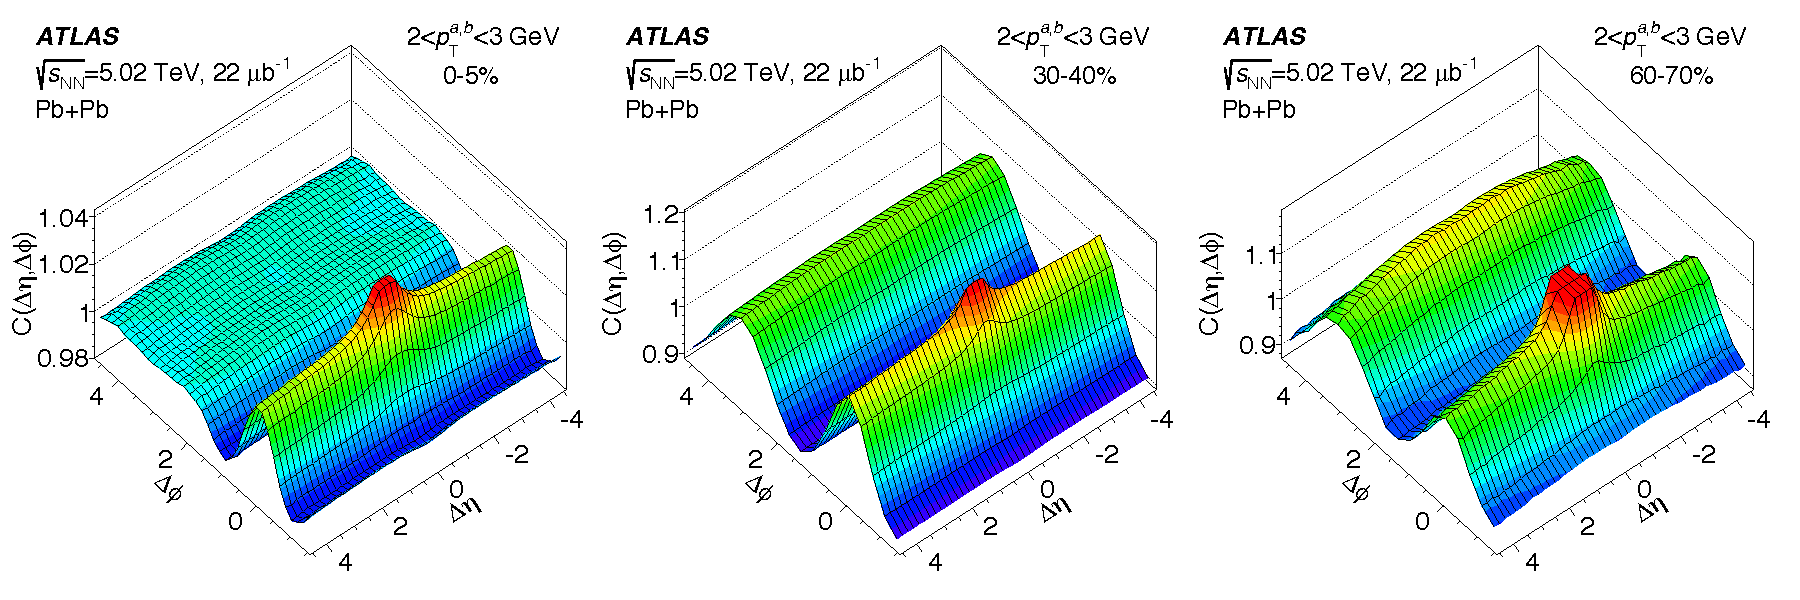
\includegraphics[width=.95\linewidth]{figs/chapter_subcumu/2pc.pdf}
\caption{Two-particle correlation function $C(\Delta\eta,\Delta\phi)$ in 5.02 TeV Pb+Pb collisions for $2<p_\text{T}^{a,b}<3$ GeV. The left, middle and right panels correspond to the 0-5\%, 30-40\% and 60-70\% centrality classes, respectively. The distributions are truncated to suppress the peak at $\Delta\eta=\Delta\phi=0$ to show the long-range correlations in greater detail. This figure is taken from Ref.~\cite{Aaboud:2018ves}.}
\label{fig:subcumu_2pc}
\end{figure}

The ridge in large systems, such as central or mid-central A+A collisions, is commonly interpreted as the result of collective hydrodynamic expansion of hot and dense nuclear matter created in the overlap region of the colliding nuclei~\cite{Abelev:2009af, ALICE:2011ab, ATLAS:2012at}. An important question about the ridge is whether it involves all particles in the event (collective flow) or if it arises merely from correlations among a few particles, due to resonance decays, jets, or multi-jet production (nonflow). Since collective flow is intrinsically a multi-particle phenomenon, it can be probed more directly using cumulants based on multi-particle correlation techniques. The ideas behind cumulant methods will be discussed in Section~\ref{sec:sub_basic_ideas}.



\subsubsection{Flow fluctuation}

In typical non-central heavy ion collisions, the large and dominating $v_2$ coefficient is associated mainly with the elliptic shape of the nuclear overlap. However, $v_2$ in central collisions and the other $v_n$ coefficients in general are related to various shape components of the initial state arising from fluctuations of the nucleon positions in the overlap region~\cite{Alver:2010gr}. The amplitudes of these shape components, characterized by eccentricity $\epsilon_n$, can be estimated via a simple Glauber model from the transverse positions $(r,\phi)$ of the participating nucleons relative to their center of mass:
\begin{equation}
\epsilon_n = \frac{\sqrt{\lr{r^n \cos n\phi}^2 + \lr{r^n \sin n\phi}^2}}{\lr{r^n}}
\end{equation}

Due to event-by-event fluctuating positions of the participants, eccentricity $\epsilon_n$ also fluctuates from event to events. Figure~\ref{fig:subcumu_Glauber_v3} shows a situation where triangle flow $\epsilon_3$ is significantly larger than $\epsilon_2$, even though the overlap region is still elliptic~\cite{Alver:2010gr}.

\begin{figure}[H]
\centering
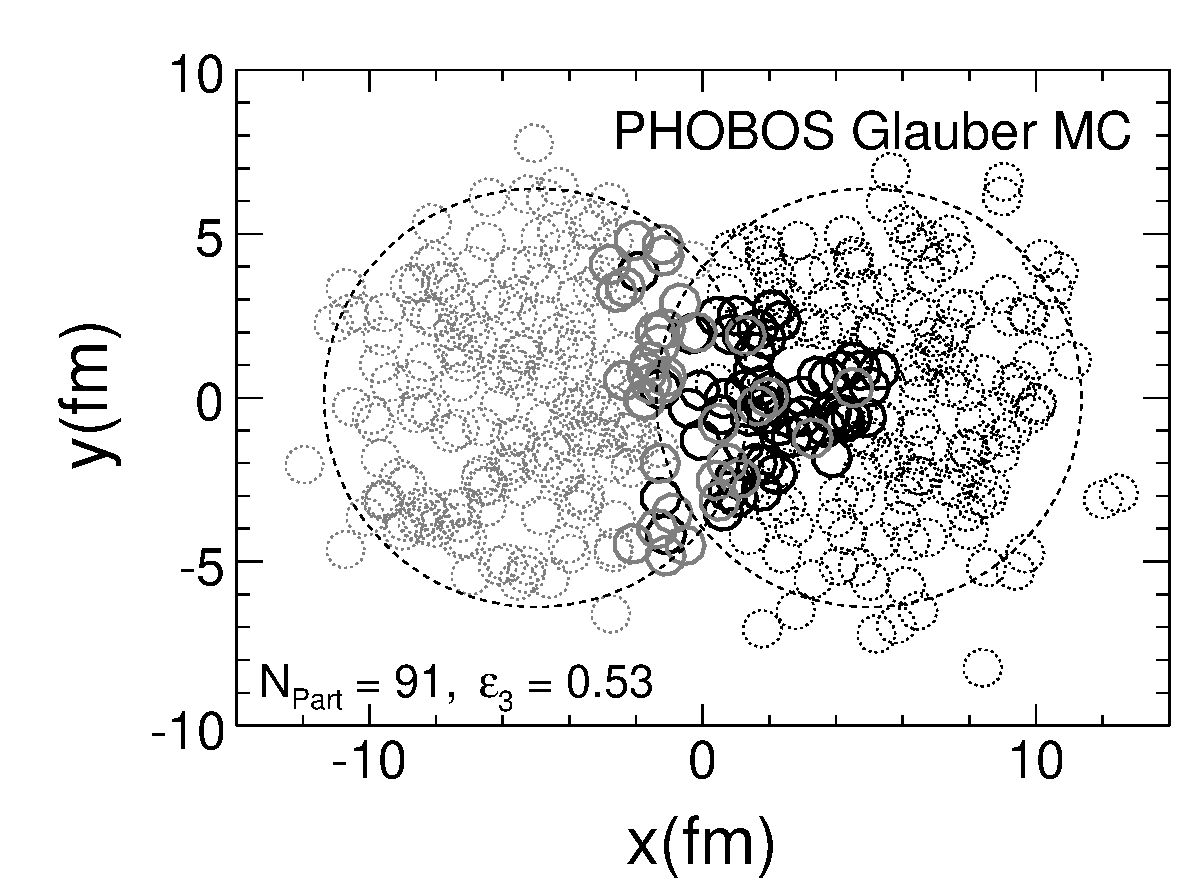
\includegraphics[width=.5\linewidth]{figs/chapter_subcumu/Glauber_v3.pdf}
\caption{Distribution of nucleons on the transverse plane for a $\sqrt{s_\text{NN}}=200$ GeV Au+Au collision event with $\epsilon_3=0.53$ from Glauber MC. The nucleons in the two nuclei are shown in gray and black. Wounded nucleons (participants) are indicated as solid circles, while spectators are dotted circles. This figure is taken from Ref.~\cite{Alver:2010gr}.}
\label{fig:subcumu_Glauber_v3}
\end{figure}

The large pressure gradients and ensuing hydrodynamic evolution can convert these shape components into $v_n$ coefficients in momentum space. Calculations based on viscous hydro-dynamics suggest that $v_n$ scales nearly linearly with $\epsilon_n$, for $n<4$. Due to significant fluctuation of $\epsilon_n$, event-by-event fluctuation of $v_n$ is also expected~\cite{Aad:2013xma}. If fluctuation of $\vec{v}_n$ relative to the underlying flow vector associated with the average geometry, $\vec{v}_n^\text{RP}$, in the reaction plane are described by a two-dimensional (2D) Gaussian function in the transverse plane, then the probability density of $\vec{v}_n$ can be expressed as:
\begin{equation}
p(\vec{v}_n) = \frac{1}{2\pi\delta_{v_n}^2}e^{-(\vec{v}_n-\vec{v}_n^\text{RP})^2/(2\delta_{v_n}^2)}
\end{equation}
where $\delta_{v_n}$ describes the width of the fluctuation. Integration of this 2D Gaussian over the azimuthal angle gives the one-dimensional (1D) probability density of $v_n=|\vec{v}_n|$ in the form of the Bessel-Gaussian function:
\begin{equation}
p(v_n) = \frac{v_n}{\delta_{v_n}^2} e^{-\frac{(v_n)^2 + (v_n^\text{RP})^2}{2\delta_{v_n}^2}} I_0(\frac{v_n^\text{RP} v_n}{\delta_{v_n}^2})
\end{equation}
where $I_0$ is the modified Bessel function of the first kind. Distribution of $v_n$ has been directly measured using unfolding technique, as shown in Figure~\ref{fig:subcumu_ebye_vn}.

\begin{figure}[H]
\centering
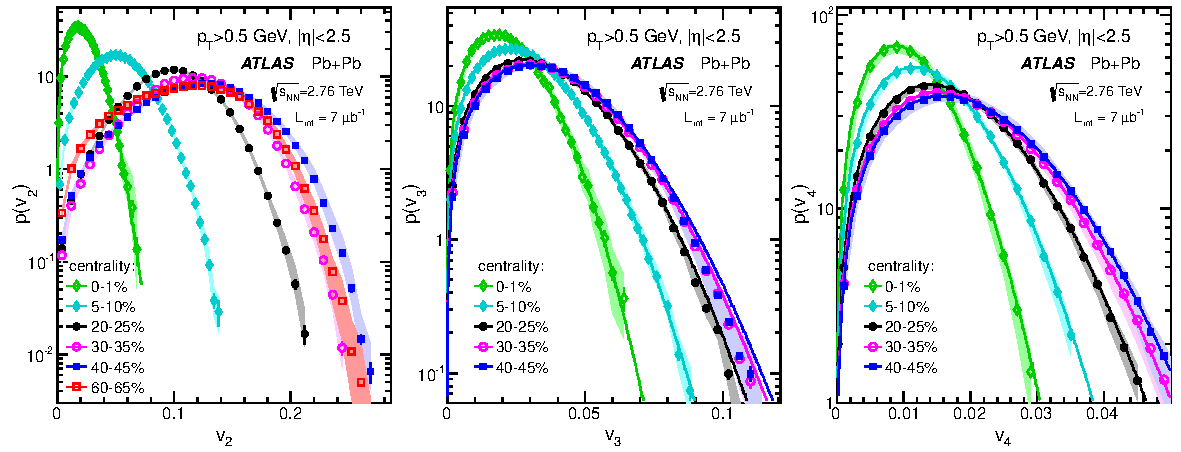
\includegraphics[width=.95\linewidth]{figs/chapter_subcumu/ebye_vn.pdf}
\caption{The probability density distributions of the event-by-event $v_n$ in several centrality intervals for n=2 (left panel), n=3 (middle panel) and n=4 (right panel). The solid curves are distributions calculated from the measured $\lr{v_n}$ according to a fluctuation-only scenario. The solid curve is shown only for $0-1\%$ centrality interval for $v_2$, but for all centrality intervals in case of $v_3$ and $v_4$. This figure is taken from Ref.~\cite{Aad:2013xma}}
\label{fig:subcumu_ebye_vn}
\end{figure}

Even though unfolding is a data-driven method, its validity relies on several assumptions and sometimes fails to converge~\cite{Aad:2013xma}. Another independent approach to probe $p(v_n)$ is through the measurements of higher-order moments of $v_n$. Cumulant method effectively measures $\lr{v_n^{2k}}$, which reflects the shape of $p(v_n)$. In addition, cumulant ratios can be used to test whether $p(v_n)$ distribution is Gaussian.



\subsection{Standard cumulant method}

The multi-particle cumulant method is used to extract the amplitude of long-range azimuthal correlations of particles produced in high-energy collisions~\cite{Borghini:2000sa}. This method has the advantage of suppressing correlations from jets and dijets, instead of relying on an explicit procedure to correct $v_n$ harmonics for dijet contributions in the 2PC approach. In this section, we will go through the basic ideas behind the standard cumulant method (its framework described in details in Ref.~\cite{Bilandzic:2010jr, Bilandzic:2013kga}), explain why it suppresses nonflow, and discuss its limitations.



\subsubsection{Basic ideas}
\label{sec:sub_basic_ideas}

The 2PC method measures correlation between particle pairs:
\begin{equation}
corr_n\{2\} = \lr{e^{\text{i}n(\phi_i-\phi_j)}} = \lr{v_n^2},
\end{equation}
where $\phi_i$ and $\phi_j$ are the azimuthal angles of two distinct particles, and $\lr{\text{ }}$ denotes the average over all particle pairs within a single event. 2PC measures the 2nd-order moment of $v_n$. Similarly, to measure the 4th-order moment, 4-particle correlation $corr_n\{4\}$ is defined as:
\begin{equation}
corr_n\{4\} = \lr{e^{\text{i}n(\phi_i+\phi_j-\phi_k-\phi_l)}},
\end{equation}
where four particles are required to be distinct from each other. 4-particle correlation can be disentangled into 2 components:
\begin{equation}
\lr{e^{\text{i}n(\phi_i+\phi_j-\phi_k-\phi_l)}} = \lr{e^{\text{i}n(\phi_i+\phi_j-\phi_k-\phi_l)}}_c + 2 \lr{e^{\text{i}n(\phi_i-\phi_k)}} \lr{e^{\text{i}n(\phi_j-\phi_l)}},
\end{equation}
where the first component (with $c$) is the genuine 4-particle correlation, meaning that all the four particles are correlated with each other. While the second component denotes the 2-particle correlations, meaning that both particle pairs $(i,k)$ and $(j,l)$ are correlated with each other, but there is no correlation between the two pairs. Note that due to symmetry, 3-particle correlations and other terms, such as $\lr{e^{\text{i}n(\phi_i+\phi_j)}}$, vanish after averaging.

Collective flow measures the global correlation among all particles, while nonflow mostly correlates smaller number of particles. To suppress these low-order correlations, 4-particle cumulant $c_n\{4\}$ is defined as:
\begin{equation}
\begin{split}
c_n\{4\} &= \lr{\lr{e^{\text{i}n(\phi_i+\phi_j-\phi_k-\phi_l)}}_c} \\
&= \lr{\lr{e^{\text{i}n(\phi_i+\phi_j-\phi_k-\phi_l)}}} - 2 \lr{\lr{e^{\text{i}n(\phi_i-\phi_k)}} \lr{e^{\text{i}n(\phi_j-\phi_l)}}} \\
&= \lr{corr_n\{4\}} - 2 \lr{corr_n\{2\}}^2 \\
&= \lr{v_n^4} - 2\lr{v_n^2}^2
\end{split}
\end{equation}
where the outer bracket $\lr{\text{ }}$ denotes the average over many similar events in a certain event class. From the definition it is obvious that 4-particle cumulant measures the genuine 4-particle correlation by subtracting the 2-particle correlations. Since it requires at least four particles to be correlated with each other, nonflow source which contains fewer than four particles are automatically suppressed.

To expand this ideas further, 6-, 8- and even higher cumulants can be defined. For example, 6-particle cumulant measures the genuine 6-particle correlation by suppressing all nonflow sources that have fewer than six particles. The 6-particle cumulant $c_n\{6\}$ is constructed as:
\begin{equation}
\begin{split}
c_n\{6\} &= \lr{corr_n\{6\}} - 9\lr{corr_n\{4\}}\lr{corr_n\{2\}} + 12\lr{corr_n\{2\}}^3 \\
&= \lr{v_n^6} - 9\lr{v_n^4}\lr{v_n^2} + 12\lr{v_n^2}^3
\end{split}
\end{equation}
where the definition becomes more complicated and more terms need to be subtracted. However, as the moment order increases, the total number of combinations decreases, and more event statistics are required to achieve sufficient measurement precision. In this thesis, up to 6-particle cumulants are measured.

While calculating $\lr{corr_n\{4\}}$, since all four particles are required to be distinct from each other, the most straightforward way is through nested loop. However, nested loop takes significant amount of time to run, and gets even worse for high-order correlations. One possible algorithm to solve the issue is the ``Q-cumulant'' technique~\cite{Bilandzic:2010jr}, which reduces the time complexity from $O(M^4)$ to $O(M)$ ($M$ is the total multiplicity). The formulas of Q-cumulant are listed in Section~\ref{sec:methodology_for_cumulant_analysis}.



\subsubsection{Limitations}

4-particle cumulant $c_n\{4\}$ can only remove the nonflow sources that have fewer than four particles. In other words, if one nonflow source has four or more particles, it still contributes to $c_n\{4\}$. For example, nonflow sources such as dijet can easily contain four or more particles. In A+A collisions, these residual nonflow contributions are diluted since the total multiplicity is much larger than four and flow contributions are dominating. However, in small systems, as the total multiplicity decreases down to less than 100, the contributions from residual nonflow are no longer negligible~\cite{Khachatryan:2015waa, Khachatryan:2016txc, Aad:2013fja, Aidala:2017ajz}.

To show that residual nonflow contributions in small systems are still significant, left panel in Figure~\ref{fig:subcumu_adam} compares $c_2\{4\}$ obtained for PYTHIA 8 with data~\cite{Aaboud:2017acw}. Since flow is not implemented in PYTHIA 8, $c_2\{4\}$ is expected to be zero. However, $c_2\{4\}$ for both model and data are observed to be larger than zero, suggesting that the residual nonflow contributions significantly bias the 4-particle cumulant measurements. Furthermore, residual nonflow contributions also make the cross-collaboration comparisons difficult. Figure~\ref{fig:subcumu_adam} compares the $c_2\{4\}$ measured by ATLAS with CMS. CMS shows that $c_2\{4\}$ is negative in the high multiplicity region, which was not observed by ATLAS. The detailed reasons for this consistency will be elaborated in Section~\ref{sec:dependence_on_the_event_class_definition}.

\begin{figure}[H]
\centering
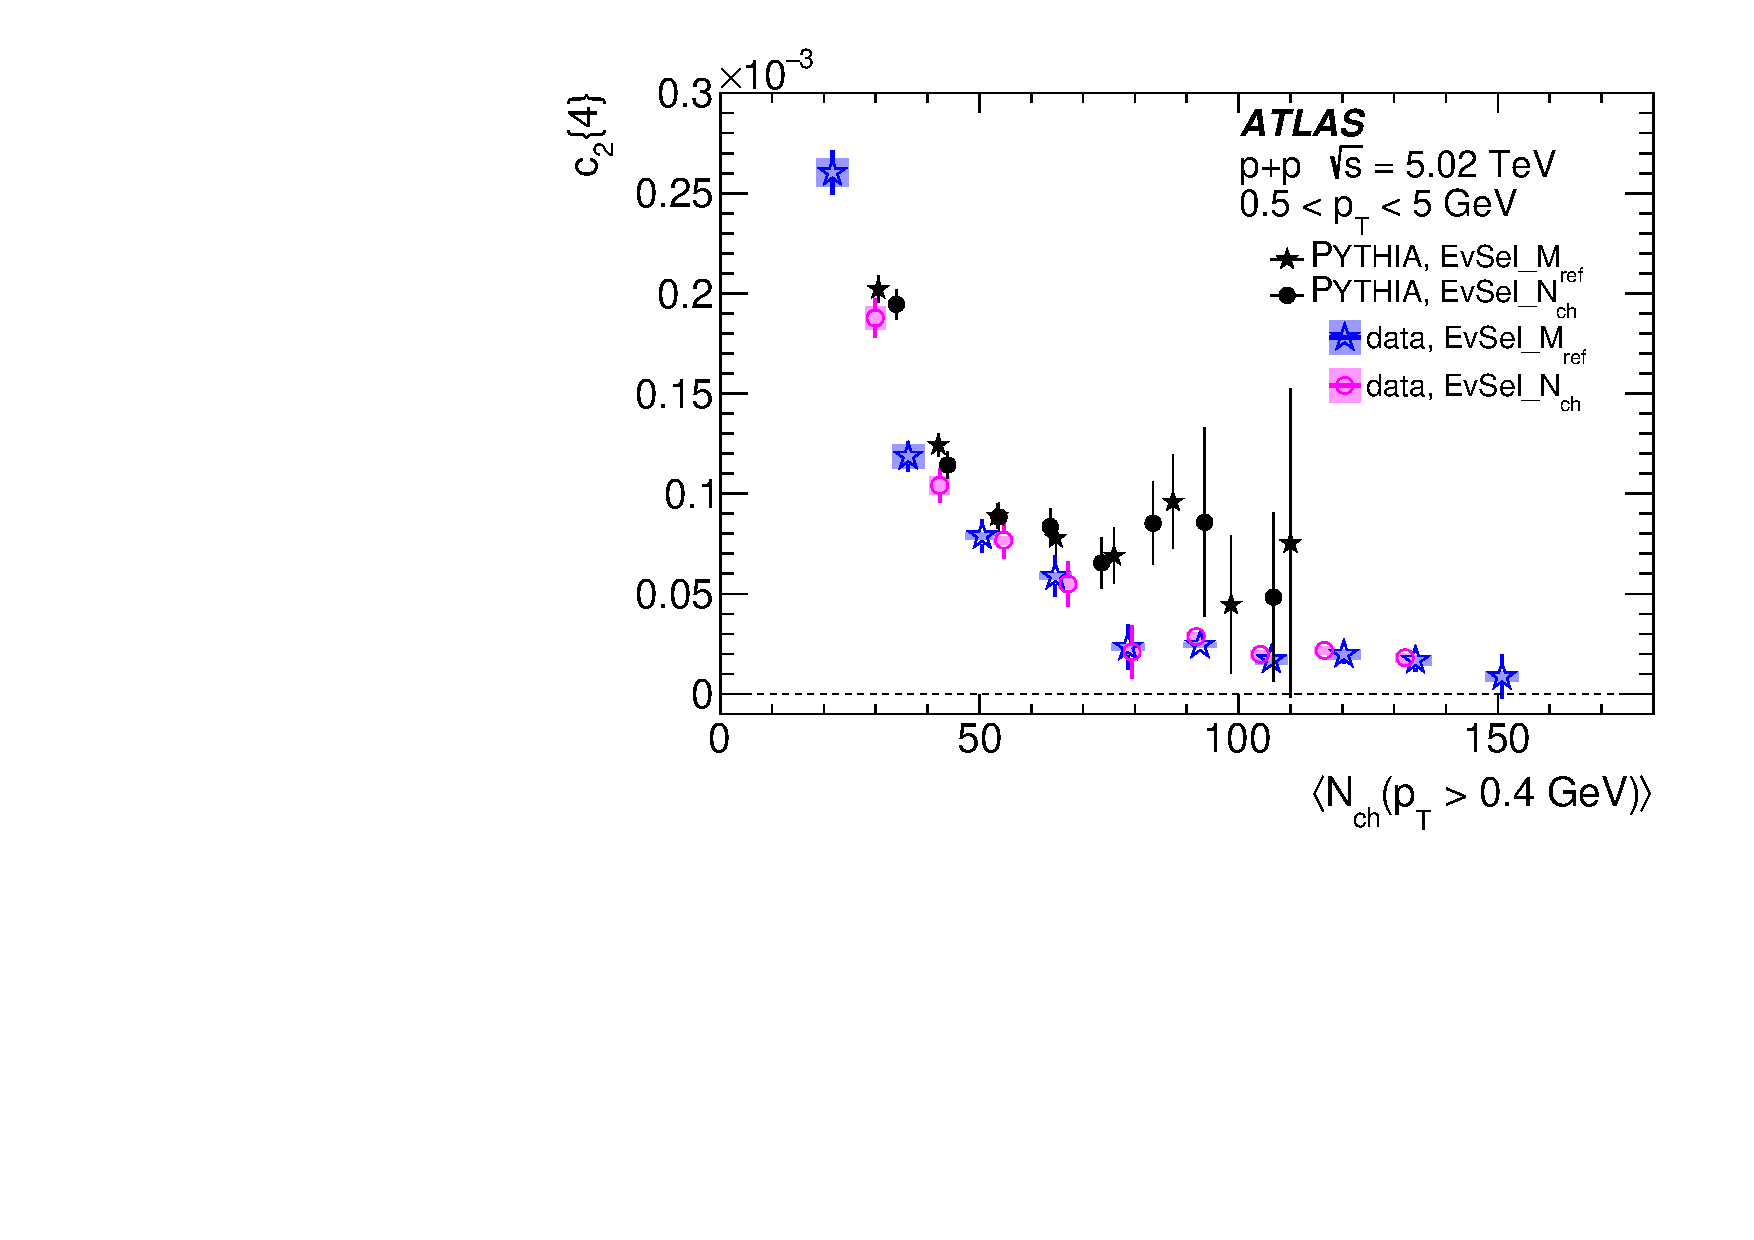
\includegraphics[width=.475\linewidth]{figs/chapter_subcumu/adam_pythia.pdf}
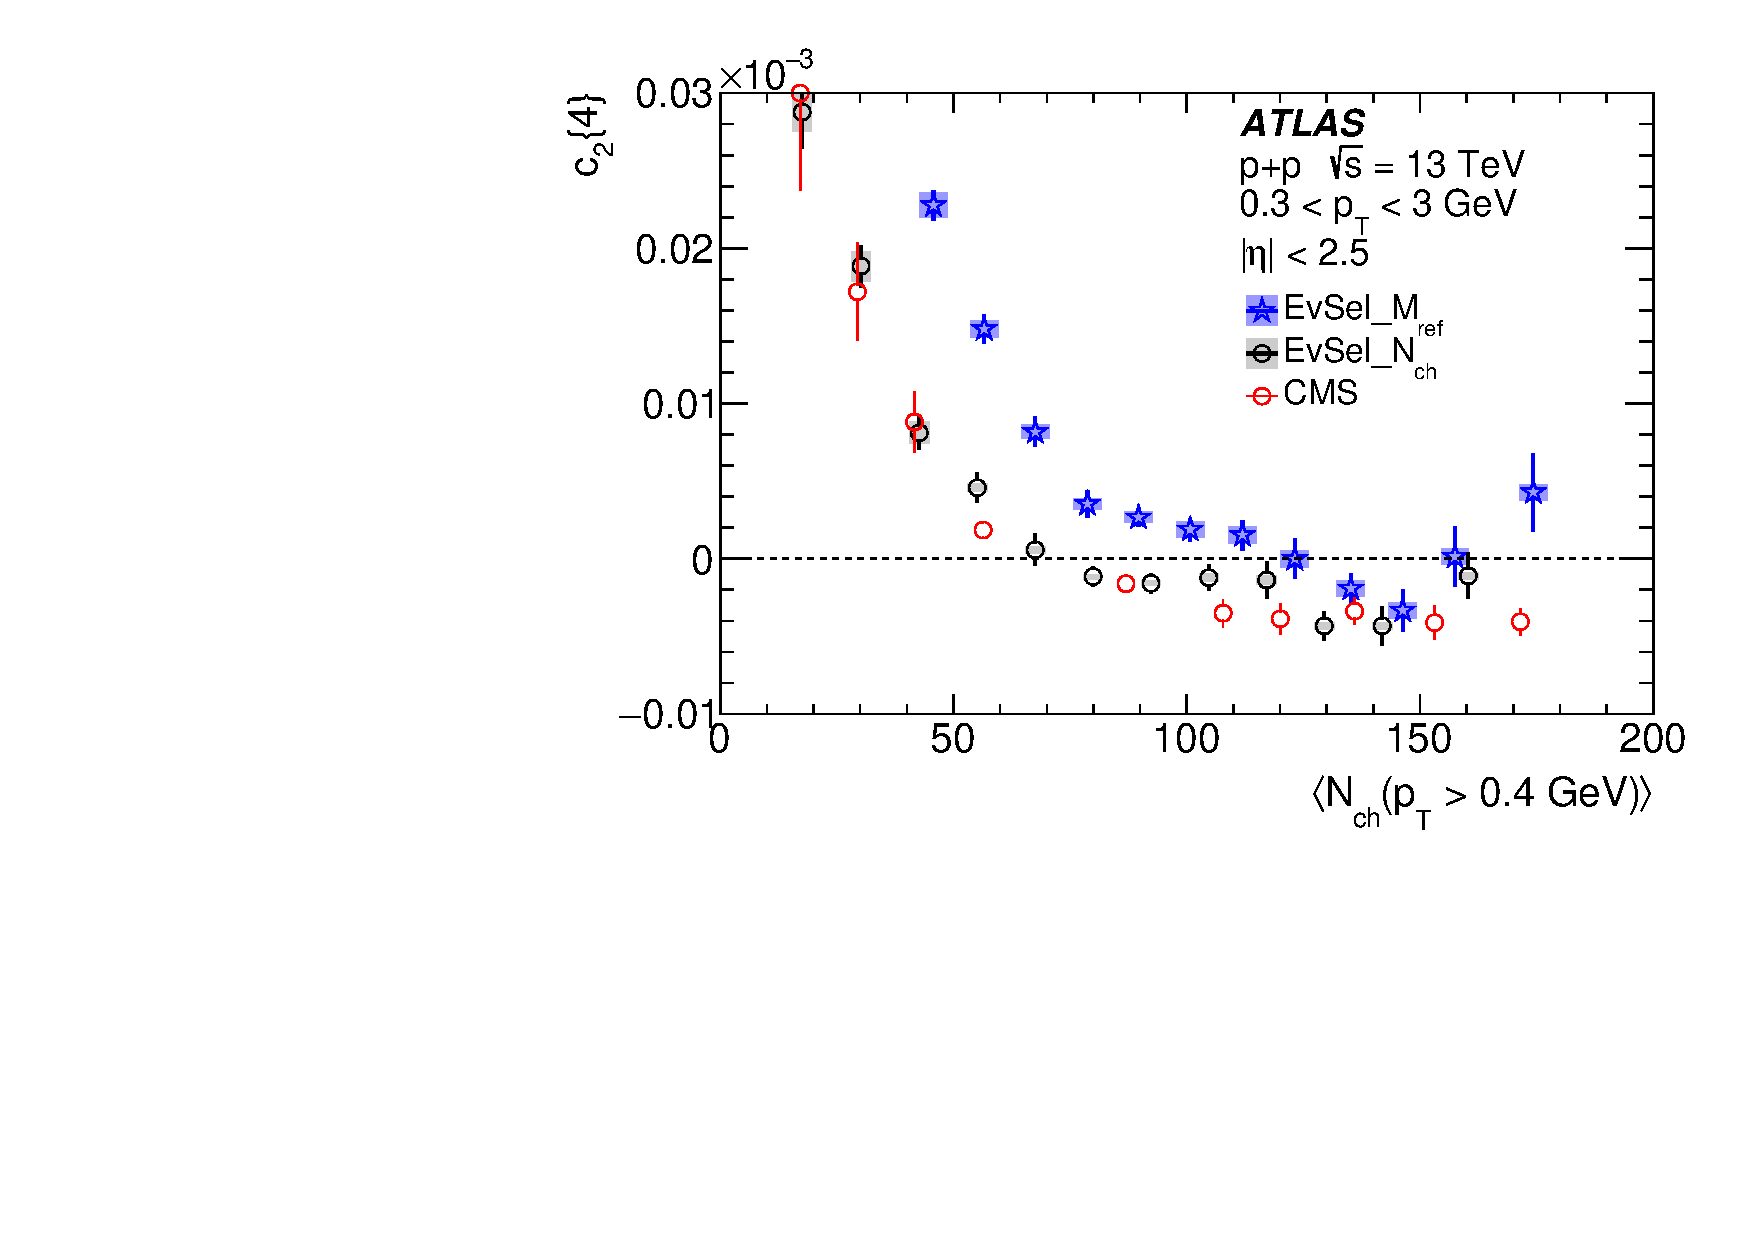
\includegraphics[width=.475\linewidth]{figs/chapter_subcumu/adam_cms.pdf}
\caption{Left: the comparison of $c_2\{4\}$ cumulants obtained for PYTHIA 8 generated $pp$ collisions at 5.02 TeV. Plots show results for reference particles with $0.5<\pT<5.0$ GeV; Right: the comparison of $c_2\{4\}$ cumulants for $pp$ collision at 13 TeV. Plots show results for reference particles with $0.3<\pT<3.0$ GeV. Both figures are taken from Ref.~\cite{Aaboud:2017acw}.}
\label{fig:subcumu_adam}
\end{figure}

One approach is solve this issue is by measuring higher-order moments, where residual nonflow contributions are further reduced. However, higher-order cumulant requires much more event statistics. Since the total multiplicity is significantly smaller in small system, the statistical error bars are much larger than large systems. Thus measuring higher-order cumulant (6-particle or higher) in small system is impractical with current event statistics.



\subsection{Subevent cumulant method}
\label{sec:subevent_cumulant_method}

To further suppress the residual nonflow correlations in small systems, newly proposed subevent cumulant method is proposed and applied in this thesis~\cite{Jia:2017hbm}. In this section, we will first go over the basic ideas behind subevent technique, explain why it will suppress nonflow. Then we will briefly list the formulas.



\subsubsection{Basic ideas}

The basic idea of subevent method is illustrated in Figure~\ref{fig:subcumu_dijet_cartoon}. Compared with standard method, in the three-subevent cumulant method the event is divided into three subevents $a$, $b$ and $c$, each covering a unique $\eta$ range, for example $-\eta_\text{max}<\eta_b<-\eta_\text{max}/3$, $|\eta_a|<\eta_\text{max}/3$, and $\eta_\text{max}/3<\eta_c<\eta_\text{max}$, where $\eta_\text{max}=2.5$ is the maximum $\eta$ used in the analysis and corresponds to the ATLAS detector acceptance for charged particles. Since the two jets in a dijet event usually produce particles in at most two subevents, the three-subevent method further suppresses nonflow contributions from inter-jet correlations associated with dijets. To enhance the statistical precision, the $\eta$ range for subevent $a$ is also interchanged with that for subevent $b$ or $c$, and the resulting three $c_2\{4\}$ values are averaged to obtain the final result.
\begin{figure}[H]
\centering
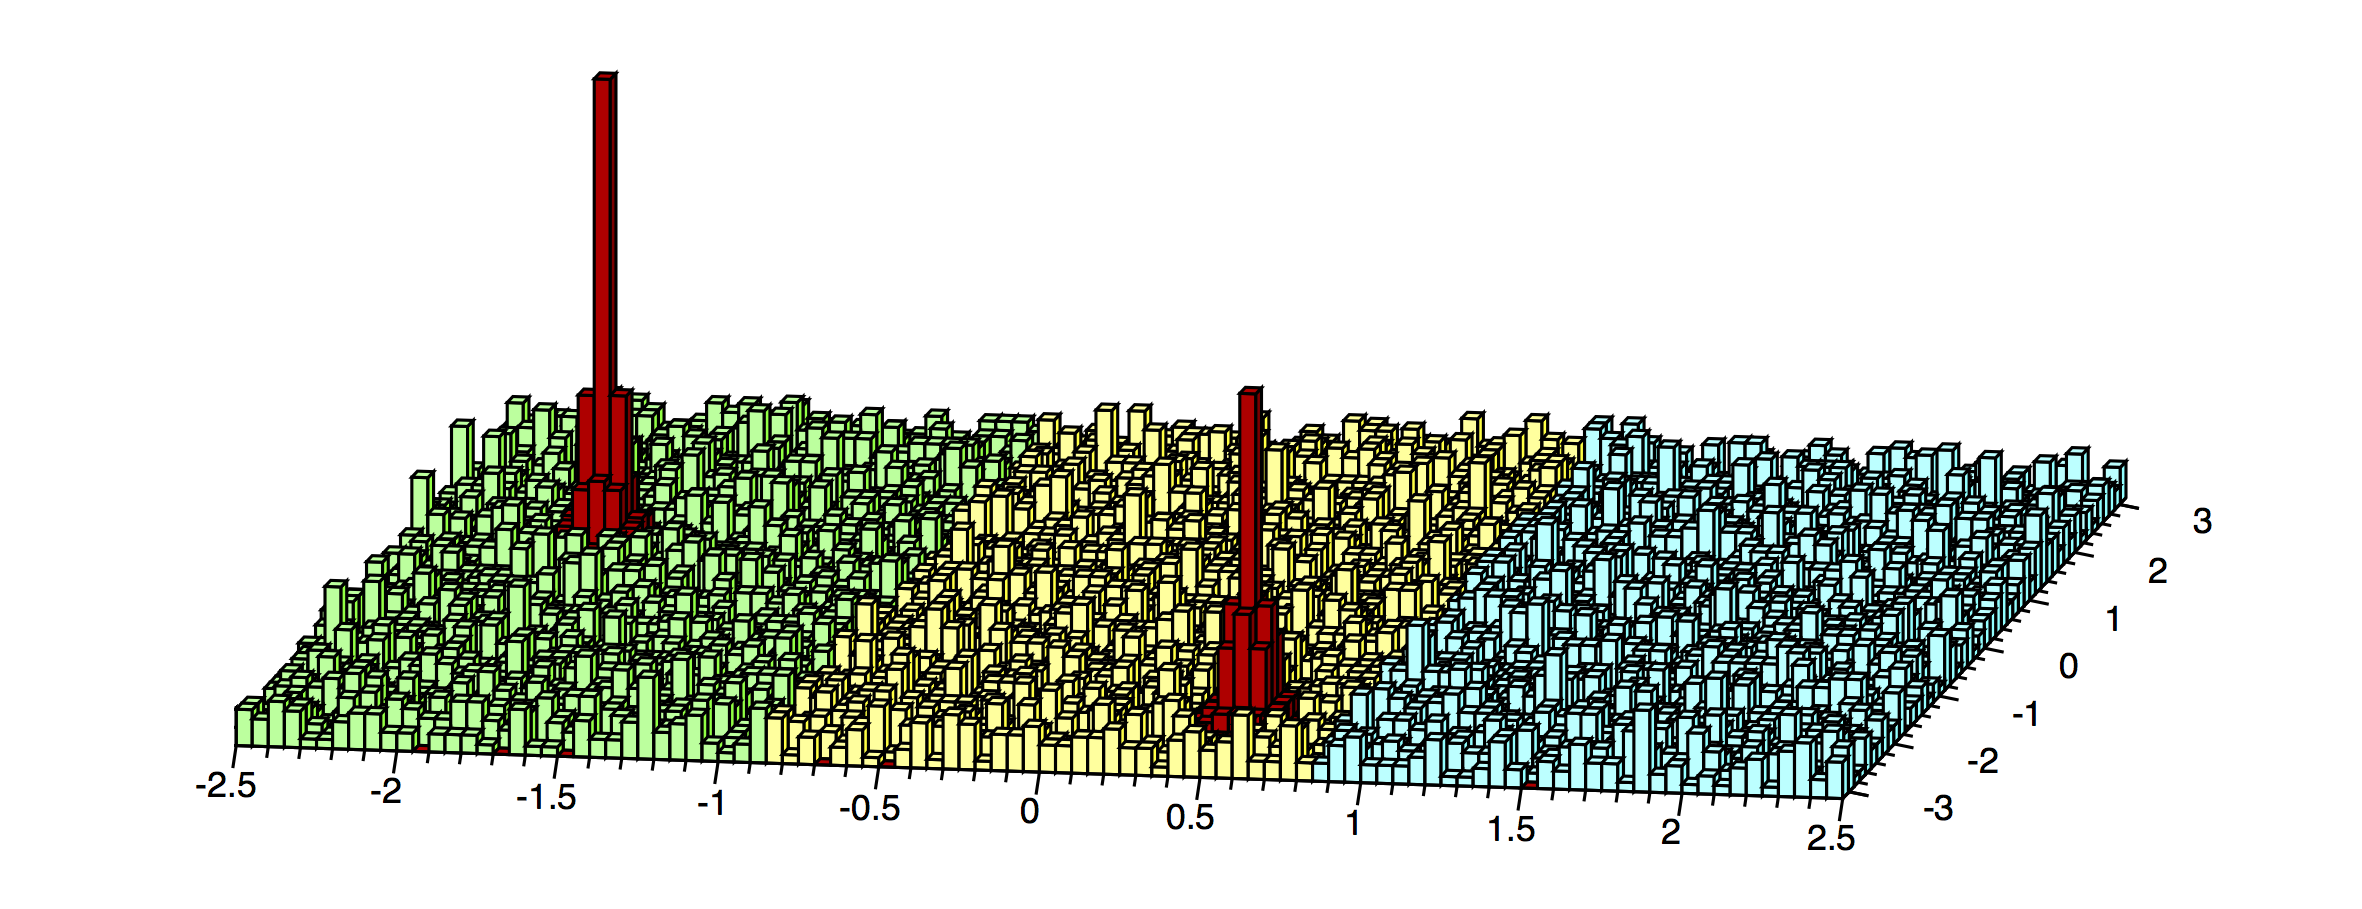
\includegraphics[width=.95\linewidth]{figs/chapter_subcumu/dijet_cartoon2.png}
\caption{Cartoon shows the dijet correlations. X-axis is $\eta$ and Y-axis is $\phi$. Particles are divided into three-subevents according to their $\eta$, as indicated by different color. The two red peaks denote particles from dijet contributions.}
\label{fig:subcumu_dijet_cartoon}
\end{figure}

Similarly, in the 2-subevent cumulant method, the entire event is divided into two subevents, labeled as $a$ and $b$, for example, according to $-\eta_\text{max}<\eta_a<0$ and $0<\eta_b<\eta_\text{max}$. The 2-subevent method should suppress correlations within a single jet (intra-jet correlations), since each jet usually emits particles into only one subevent.

The only drawback of subevent method is that its statistical significance is worse than standard method, since it not only removes the particle combinations from nonflow sources, but also suppresses those from flow contributions. This is like treating cancer with chemotherapy: it not only kills the cancer cells, but also kills the healthy ones. However, until the perfect cure for suppressing nonflow is found, we will stick to subevent method.



\subsubsection{Methodology}

To separate from standard method, we use superscript $a$, $b$ and $c$ to represent three subevents. The 2- and 4-particle correlation are then written as:
\begin{equation}
\begin{split}
corr_n^{b|c}\{2\} &= \lr{e^{\text{i}n(\phi_b-\phi_c)}} \\
corr_n^{a,a|b,c}\{2\} &= \lr{e^{\text{i}n(\phi_a+\phi_a-\phi_b-\phi_c)}}
\end{split}
\end{equation}
where $|$ is used to denote the sign before $\phi$ for each particle. Note that all particles are still required to be distinct from each other. $corr_n^{a,a|b,c}\{2\}$ can also be calculated using Q-cumulant technique, and the formulas are summarized in Section~\ref{sec:methodology_for_cumulant_analysis}.

The 2- and 4-particle three-subevent cumulants are defined as:
\begin{equation}
\begin{split}
c_n^{b|c}\{2\} &= \lr{corr_n^{b|c}\{2\}} \\
c_n^{a,a|b,c}\{4\} &= \lr{corr_n^{a,a|b,c}\{4\}} - 2\lr{corr_n^{a|b}\{2\}}\lr{corr_n^{a|c}\{2\}}
\end{split}
\end{equation}
where the formulas are similar to standard method, but with superscripts added.

Different order cumulants provide independent estimates for the same reference harmonic $v_n$. If the underlying $v_n$ fluctuation is Bessel-Gaussian or close to Bessel-Gaussian (e.g. power-law function), then the 2- and 4-particle cumulants can be expanded as~\cite{Voloshin:2007pc}:
\begin{equation}
\begin{split}
c_n\{2\} &= \bar{v}_n^2 + 2\delta_n^2 \\
c_n\{4\} &= -\bar{v}_n^4
\end{split}
\end{equation}
where $\bar{v}_n$ denotes the mean value of $v_n$ and $\delta_n$ describes the Gaussian fluctuation width of $v_n$. Thus 2- and 4-particle flow signal $v_n\{2\}$ and $v_n\{4\}$ for the corresponding cumulants can be defined as:
\begin{equation}
\begin{split}
v_n\{2\} &= \sqrt{c_n\{2\}} \\
v_n\{4\} &= \sqrt[4]{-c_n\{4\}}
\end{split}
\end{equation}



\subsection{Results}

In the results section, we applied both standard and subevent cumulant methods to the PYTHIA MC samples and the ATLAS data. The purpose of PYTHIA studies is to validate the subevent method, showing that it can suppress nonflow as designed. While we use data to probe collective flow in the small systems.



\subsubsection{PYTHIA model}

\paragraph{Simulation setup}

Particle production in $pp$ collisions is often described by QCD-inspired models implemented in MC event generators such as PYTHIA~\cite{Sjostrand:2007gs}. The PYTHIA model contains significant nonflow correlations from jets, dijets and resonance decays but has no genuine long-range ridge correlations. In this study, 200 million $pp$ collisions at $\sqrt{s}=13$ TeV are generated with PYTHIA 8. Multi-particle cumulants based on standard method as well as subevent methods are calculated to quantify how they are biased by nonflow correlations as a function of charged particle multiplicity. Furthermore, flow signal is added to the generated event using a flow afterburner~\cite{Masera:2009zz}, and the performance of recovering the input flow signal is studied.

In a typical azimuthal correlation analysis, multi-particle correlators $corr_n\{2k\}$ are calculated for particles passing selection criteria $X_1$, and are then averaged over many events with the same number of charged particles $\Nch$ passing other selection criteria $X_2$ to obtain $\lr{corr_n\{2k\}}$ and then $c_n\{2k\}$. In order to present the cumulants along a common $x$ axis, the $\Nch$ based on criteria $X_2$ is often mapped to a common event activity measure, typically $\Nch$ passing yet another criterion $X_3$. If nonflow is sufficiently suppressed, $c_n\{2k\}$ should measure the collectivity of the entire event and therefore should not depend on the intermediate criteria $X_2$. However, the ATLAS Collaboration observed that $c_2\{4\}$ calculated in both PYTHIA and with $pp$ data depends sensitively on criteria $X_2$~\cite{Aaboud:2017acw}, as shown in the right panel of Figure~\ref{fig:subcumu_adam}, where ATLAS and CMS used different criteria for $X_2$. The reason for such sensitivity was thought to arise from relative multiplicity fluctuation between $X_2$ and $X_3$. The real reason, as we shall argue below, is due to change in event-by-event nonflow distribution. We show that the three-subevent method nearly completely removes nonflow contributions, such that the resulting $c_2\{4\}$ is independent of $X_2$.

In order to study this effect in PYTHIA, we tested different $\pT$ thresholds for $X_1$, $X_2$ and $X_3$, and they are summarized below:
\begin{itemize}
\item $X_1$: $0.3<\pT<3.0$ GeV; $0.5<\pT<5.0$ GeV;
\item $X_2$: same as $X_1$; $\pT>0.2$ GeV; $\pT>0.4$ GeV; $\pT>0.6$ GeV;
\item $X_3$: $\pT>0.4$ GeV
\end{itemize}
For each method, cumulants are calculated in two $\pT$ ranges ($X_1$) for event classes defined by the number of charged particles in four $\pT$ ranges ($X_2$), denoted by $\Nchsel$. For each combination, the $c_n\{2k\}$ are calculated for events with a fixed $\Nchsel$ multiplicity; the results for one-particle-width bins in $\Nchsel$ are then combined to broader $\Nchsel$ intervals. When presenting the final results, the $\lr{\Nchsel}$ values for given $\Nchsel$ interval are mapped to the average number of charged particles with $\pT>0.4$ GeV ($X_3$), denoted by $\lr{\Nch}$. For $X_2$, ATLAS selected same $\pT$ threshold as $X_1$, while CMS used $\pT>0.4$ GeV, same as $X_3$.



\paragraph{Dependence on the event-class definition}

Left panel of Figure~\ref{fig:subcumu_PYTHIA_c24_pT0_X2} shows the four-particle cumulants obtained with the standard method using charged particles in $0.3<\pT<3.0$ GeV. The $c_2\{4\}$ values are found to differ significantly between the four choices of $\Nchsel$, therefore confirming the observation made by the ATLAS Collaboration~\cite{Aaboud:2017acw}. The red and blue dashed lines indicate expected $c_n\{4\}$ values corresponding to $4\%$ and $6\%$ flow signal. Clearly nonflow contributions in the standard method are too large for a meaningful measurement of $v_2$. In fact, when $\Nchsel$ is defined in the $\pT$ range of $\pT>0.6$ GeV, the sign of $c_2\{4\}$ is negative at small $\lr{\Nch}$ values.

Right panel of Figure~\ref{fig:subcumu_PYTHIA_c24} shows $c_n\{4\}$ obtained from the three-subevent methods. The three-subevent method almost completely suppresses the nonflow. For $c_2\{4\}$, the magnitude of the residual nonflow are less than $4\%$ of flow signal. This means that the three-subevent method should be sensitive to genuine long-range flow signal as small as $4\%$.

\begin{figure}[H]
\centering
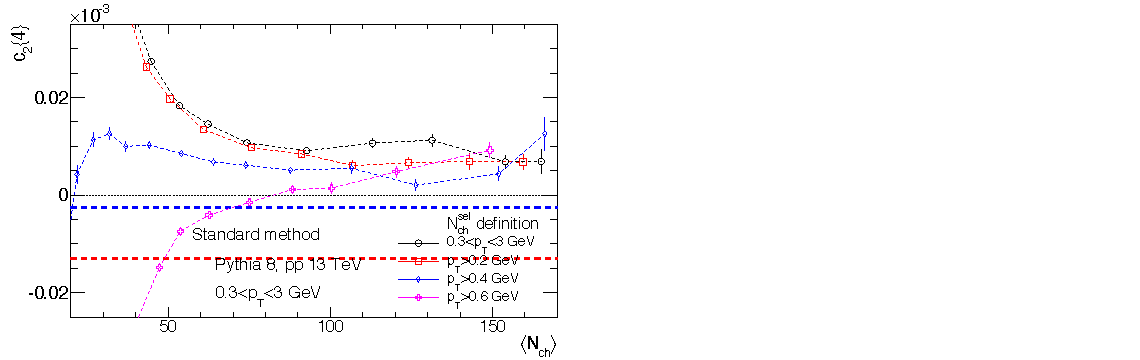
\includegraphics[width=.475\linewidth]{figs/chapter_subcumu/PYTHIA_c24_pT0_std_X2}
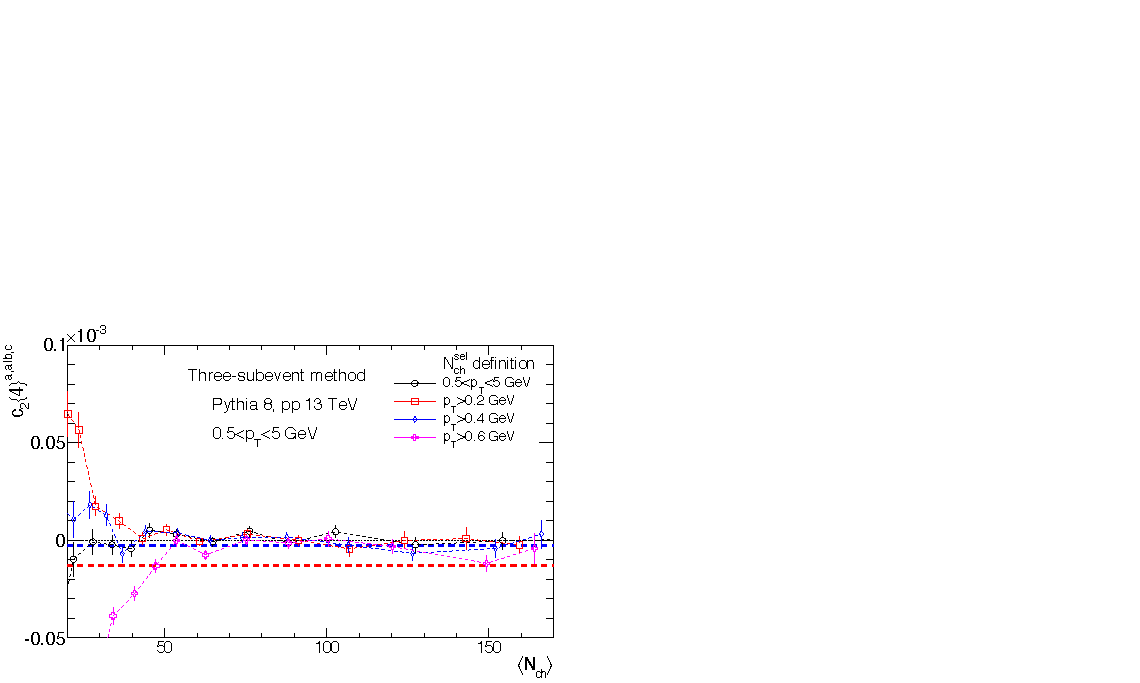
\includegraphics[width=.475\linewidth]{figs/chapter_subcumu/PYTHIA_c24_pT0_sub_X2}
\caption{The $c_2\{4\}$ calculated for particles in $0.3<\pT<3.0$ GeV with the standard (left panel) and the subevent (right panel) cumulant method. The event averaging is performed for $\Nchsel$ calculated for various $\pT$ selections as indicated in the figure, which is then mapped to $\lr{\Nch}$, the average number of charged particles with $\pT>0.4$ GeV.}
\label{fig:subcumu_PYTHIA_c24_pT0_X2}
\end{figure}



\paragraph{Comparison between different cumulant methods}

Figure~\ref{fig:subcumu_PYTHIA_c24} shows a direct comparison between the standard method and the two- and three-subevent methods for $c_2\{4\}$ in two $\pT$ ranges. The three-subevent method has the best performance in suppressing the nonflow effects.

\begin{figure}[H]
\centering
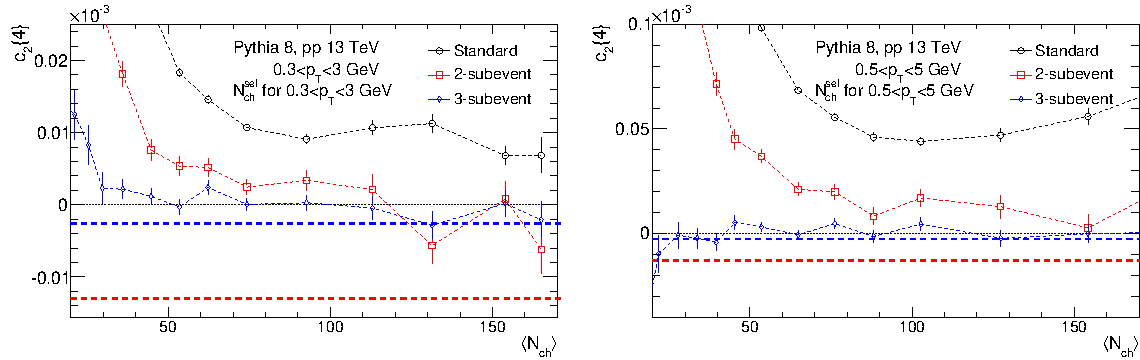
\includegraphics[width=.95\linewidth]{figs/chapter_subcumu/PYTHIA_c24}
\caption{The $c_2\{4\}$ calculated for particles in $0.3<\pT<3.0$ GeV (left panel) or $0.5<\pT<5.0$ GeV (right panel) compared between the three cumulant methods. The event averaging is performed for $\Nchsel$ calculated for same $\pT$ range, which is then mapped to $\lr{\Nch}$, the average number of charged particles with $\pT>0.4$ GeV.}
\label{fig:subcumu_PYTHIA_c24}
\end{figure}

To quantify the performance of the three methods for recovering the underlying flow signal, a flow afterburner~\cite{Masera:2009zz} is used to add a constant $v_2$ or $v_3$ signal to the generated PYTHIA events. Figure~\ref{fig:subcumu_PYTHIA_c24_ab} shows the calculated $c_2\{4\}$ with $4\%$ or $6\%$ $v_2$ imposed on the generated events. In the case $4\%$ input flow, only the three-subevent method can recover the input. In the case of $6\%$ input flow, the two-subevent method can also recover the input flow for $\lr{\Nch}>80$.

\begin{figure}[H]
\centering
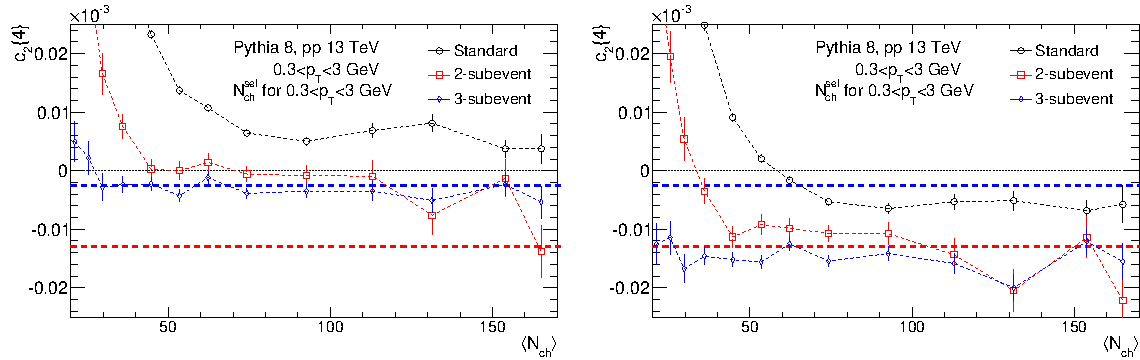
\includegraphics[width=.95\linewidth]{figs/chapter_subcumu/PYTHIA_c24_ab}
\caption{The $c_2\{4\}$ calculated for particles in $0.3<\pT<3.0$ GeV compared among the three cumulant methods with $4\%$ (left panel) or $6\%$ (right panel) $v_2$ imposed. The event averaging is performed for $\Nchsel$ calculated for same $\pT$ range, which is then mapped to $\lr{\Nch}$, the average number of charged particles with $\pT>0.4$ GeV.}
\label{fig:subcumu_PYTHIA_c24_ab}
\end{figure}



\paragraph{Bin width effects}

In the cumulant analysis, it has been argued that $c_n\{2k\}$ should be calculated for each fixed $\Nchsel$ bin to minimize the event-by-event variation of particle multiplicity, then should be averaged over broader $\Nchsel$ intervals~\cite{Bilandzic:2010jr, Chatrchyan:2013nka}. Figure~\ref{fig:subcumu_PYTHIA_c24_binWidth} shows $c_2\{4\}$ for charged particles in $0.3<\pT<3.0$ GeV for events with $40<\Nch<80$, where $\Nch$ is the number of charged particles also in $0.3<\pT<3.0$ GeV. The $c_2\{4\}$ values are obtained with $\Nch$ bin widths of 1, 5, 10, 20 and 40, respectively. The $c_2\{4\}$ values for each case are then averaged over the $40<\Nch<80$ interval to give a single $c_2\{4\}$ value. The difference of $c_2\{4\}$ for a given bin width from $c_2\{4\}$ for unit bin width is then plotted. Clearly, the standard method is much more sensitive to the bin width than the two-subevent and three-subevent methods. This sensitivity is due to the fact that the standard method still has significant nonflow, whose event-by-event fluctuation also has significant non-Gaussianity. Therefore the residual nonflow has significant dependence on the bin width in the standard method. On the other hand, since nonflow contributions are significantly further suppressed in the subevent methods, the nature of the nonflow fluctuations no longer matter much for the subevent methods.

\begin{figure}[H]
\centering
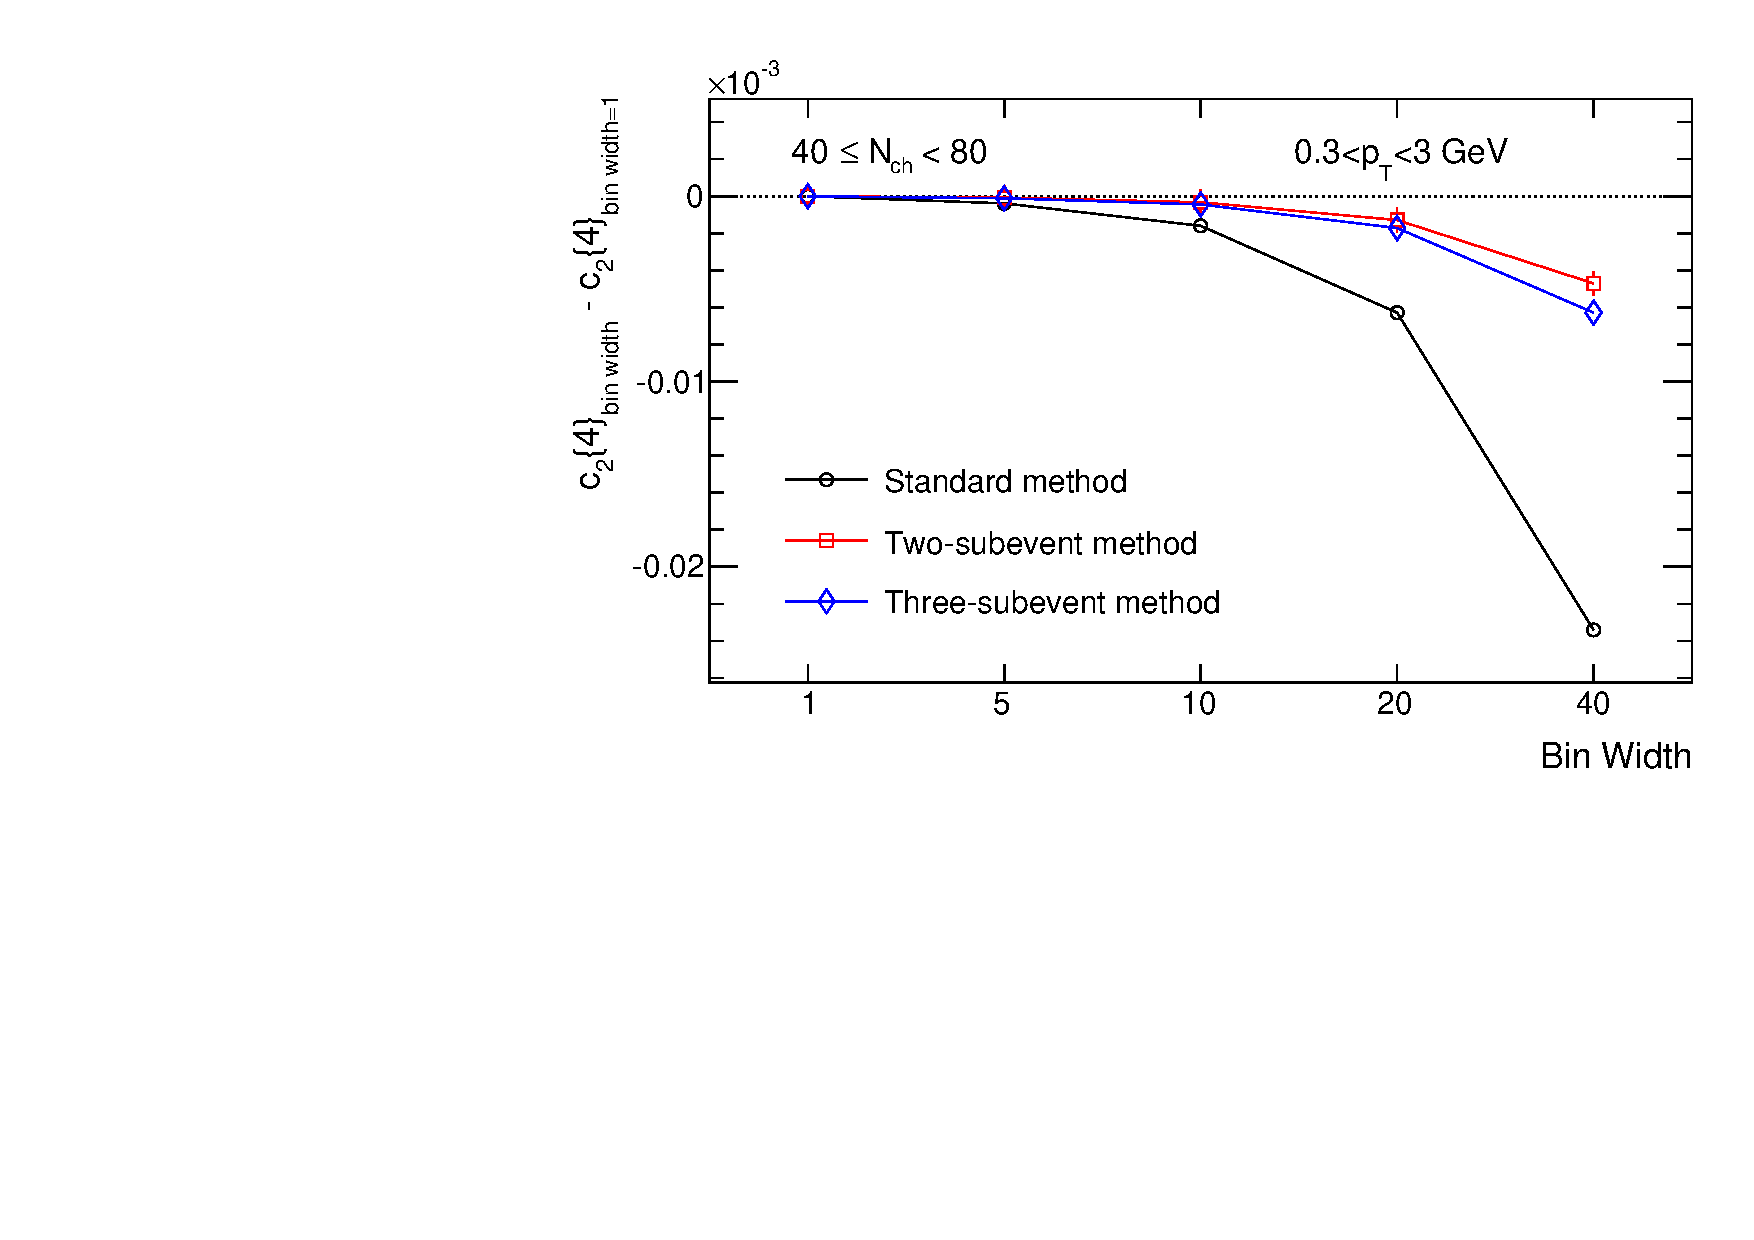
\includegraphics[width=.6\linewidth]{figs/chapter_subcumu/PYTHIA_c24_binWidth}
\caption{The $c_2\{4\}$ calculated in different bin widths of $\Nch (0.3<\pT<3.0\text{ GeV})$ then averaged over the $40<\Nch<80$ interval. The difference from the unit-bin-width case is plotted as a function of bin width.}
\label{fig:subcumu_PYTHIA_c24_binWidth}
\end{figure}



\subsubsection{ATLAS data}

\paragraph{Dependence on the event-class definition}
\label{sec:dependence_on_the_event_class_definition}

This section presents the sensitivity of $c_2\{4\}$ to $\Nchsel$, which defines the event class used to calculate $\lr{corr_n\{2k\}}$. The discussion is based on results obtained from the 13 TeV $pp$ data, but the observations for the 5.02 TeV $pp$ and $p$+Pb data are qualitatively similar.

Left panel of Figure~\ref{fig:subcumu_ATLAS_c24_pT0_X2} shows the $c_2\{4\}$ values obtained using the standard method for four event-class definitions based on $\Nchsel$. The $c_2\{4\}$ values change dramatically as the event-class definition is varied, which reflects different amount of nonflow fluctuations associated with different $\Nchsel$. Similar behaviours are observed in the PYTHIA studies above. The $c_2\{4\}$ values for $0.3<\pT<3.0$ GeV become negative when the reference $\Nchsel$ is obtained for $\pT>0.4$ GeV or higher, but the four cases do not converge to the same $c_2\{4\}$ values. These behaviors suggest that the $c_2\{4\}$ values from the standard method are strongly influenced by nonflow effects in all $\lr{\Nch}$ and $\pT$ ranges. Therefore the previously observed negative $c_2\{4\}$ in $pp$ collisions for $0.3<\pT<3.0$ GeV and $\Nchsel$ with $\pT>0.4$ GeV~\cite{Khachatryan:2016txc} may be dominated by nonflow correlations instead of long-range collective flow.

Right panel of Figure~\ref{fig:subcumu_ATLAS_c24_pT0_X2} shows the results from the three-subevent method. For most of the $\lr{\Nch}$ range, the $c_2\{4\}$ values are negative, i.e., having the sign expected for long-range ridge correlations. The $c_2\{4\}$ values show some sensitivity to the definition of the reference $\Nchsel$ but they are close to each other for all definitions in the region $\lr{\Nch}>100$. This suggests that the residual nonflow effects may still be important at small $\lr{\Nch}$, but are negligible at $\lr{\Nch}>100$. It is also observed that the $c_2\{4\}$ values for $0.5<\pT<5.0$ GeV are more negative than those for $0.3<\pT<3.0$ GeV~\cite{Aaboud:2017blb}, which is consistent with the observation that the $v_2$ value associated with the long-range collectivity increases with $\pT$~\cite{Aad:2014lta, Aaboud:2016yar}.

Given the relatively small dependence of $c_2\{4\}$ on the reference $\Nchsel$ in the three-subevent method, the remaining discussion focuses on cases there the reference $\Nchsel$ is calculated in the same $\pT$ ranges as those used for calculating $c_2\{4\}$, i.e., $0.3<\pT<3.0$ GeV and $0.5<\pT<5.0$ GeV.

\begin{figure}[H]
\centering
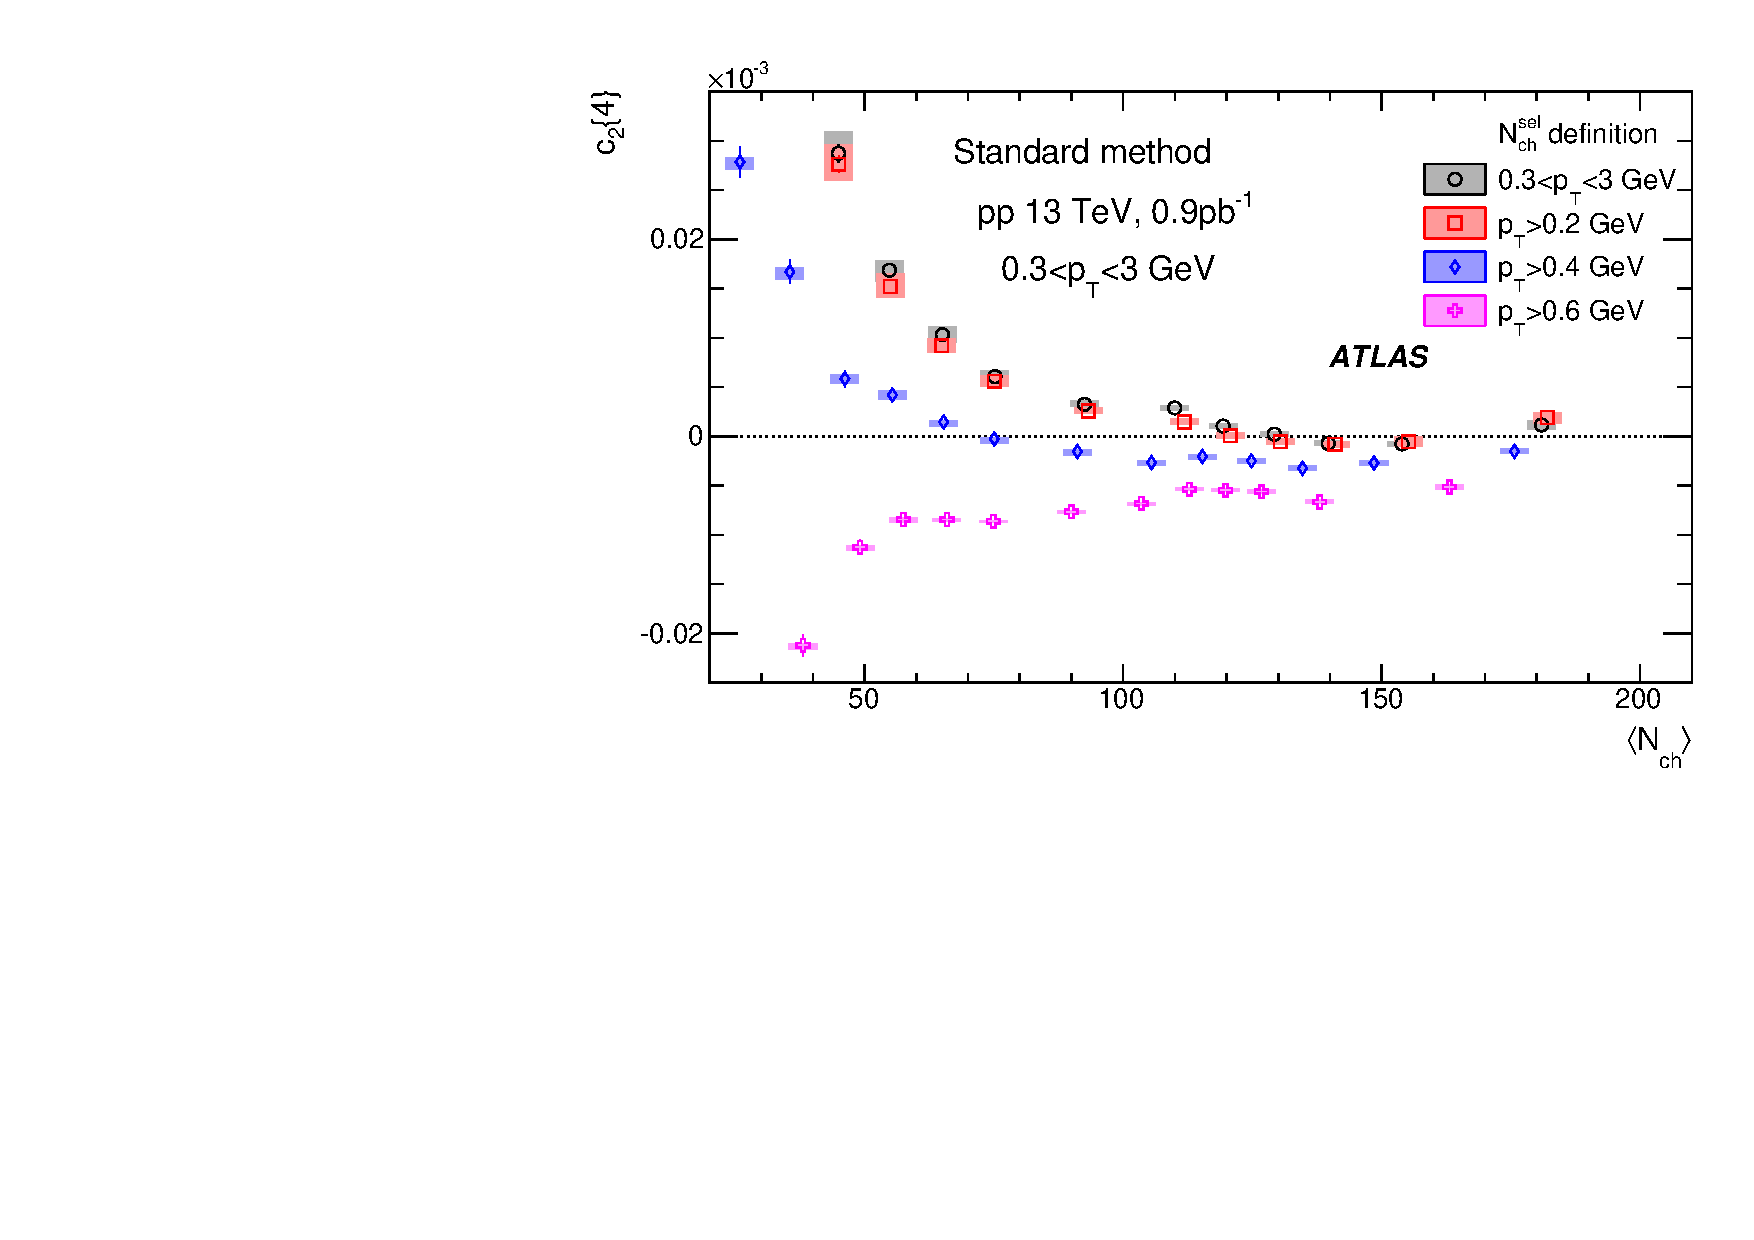
\includegraphics[width=.475\linewidth]{figs/chapter_subcumu/ATLAS_c24_pT0_std_X2}
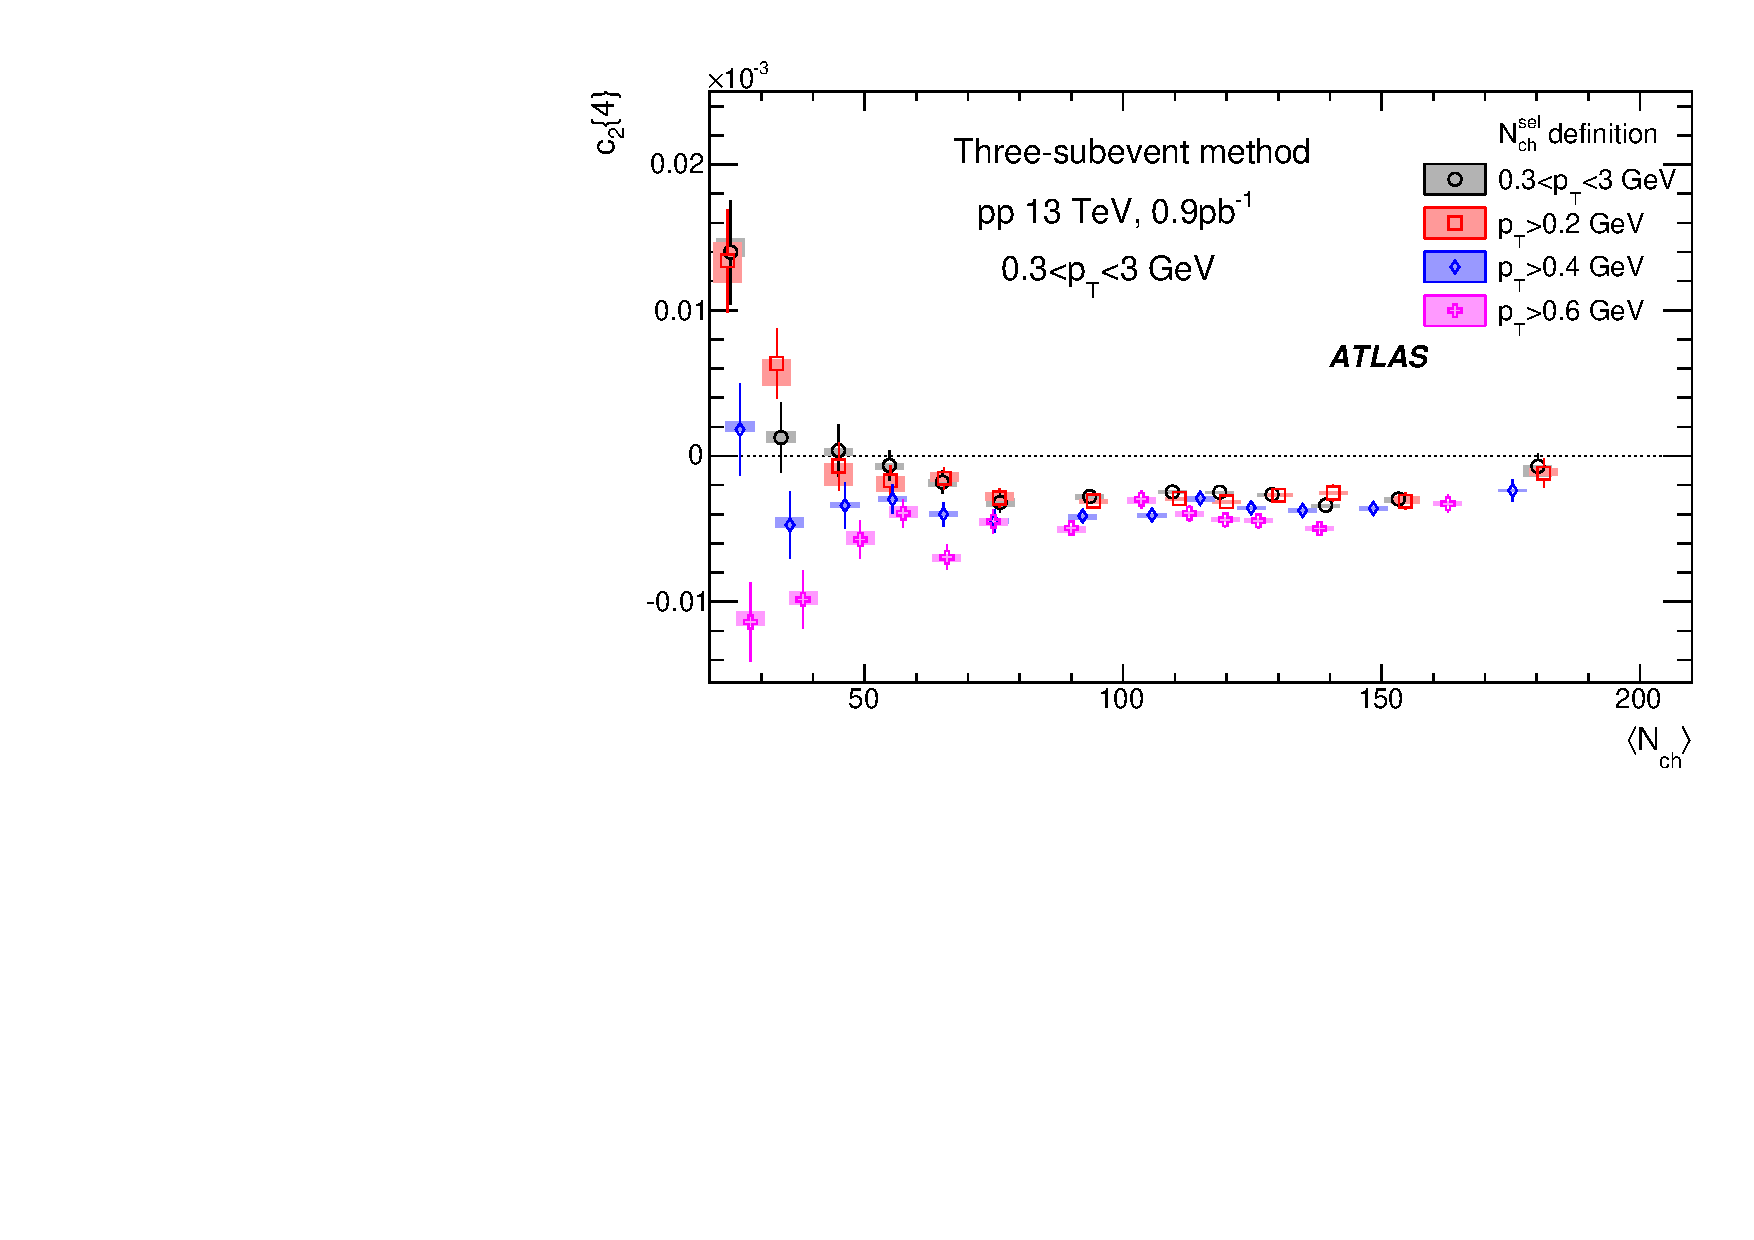
\includegraphics[width=.475\linewidth]{figs/chapter_subcumu/ATLAS_c24_pT0_sub_X2}
\caption{The $c_2\{4\}$ values calculated for charged particles with $0.3<\pT<3.0$ GeV with the standard (left panel) and subevent (right panel) cumulant method from the 13 TeV $pp$ data. The event averaging is performed for $\Nchsel$ calculated for various $\pT$ selections as indicated in the figure, which is then mapped to $\lr{\Nch}$, the average number of charged particles with $\pT>0.4$ GeV. The error bars and shaded boxes represent the statistical and systematic uncertainties, respectively.}
\label{fig:subcumu_ATLAS_c24_pT0_X2}
\end{figure}



\paragraph{Comparison between different cumulant methods}
\label{comparison_between_different_cumulant_methods}

Figures~\ref{fig:subcumu_ATLAS_c24_pp13}-\ref{fig:subcumu_ATLAS_c24_pPb5} show direct comparisons of the results for the standard, two-subevent, and three-subevent methods for $pp$ collisions at $\sqrt{s}=13$ TeV, $pp$ at $\sqrt{s}=5.02$ TeV and $p$+Pb collisions at $\sqrt{s_\text{NN}}=5.02$ TeV, respectively. The results from 5.02 TeV $pp$ collisions are qualitatively similar to those from the 13 TeV $pp$ collisions, i.e., the $c_2\{4\}$ values are smallest for the three-subevent method and largest for the standard method. The same hierarchy between three methods is also observed in $p$+Pb collisions, but only for the $\lr{\Nch}<100$ region, suggesting that nonflow effects in $p$+Pb collisions are much smaller than those in $pp$ collisions at comparable $\lr{\Nch}$. In $p$+Pb collisions, all three methods give consistent results for $\lr{\Nch}>100$. Furthermore, the three-subevent method gives negative $c_2\{4\}$ values in most of the measured $\lr{\Nch}$ range.

\begin{figure}[H]
\centering
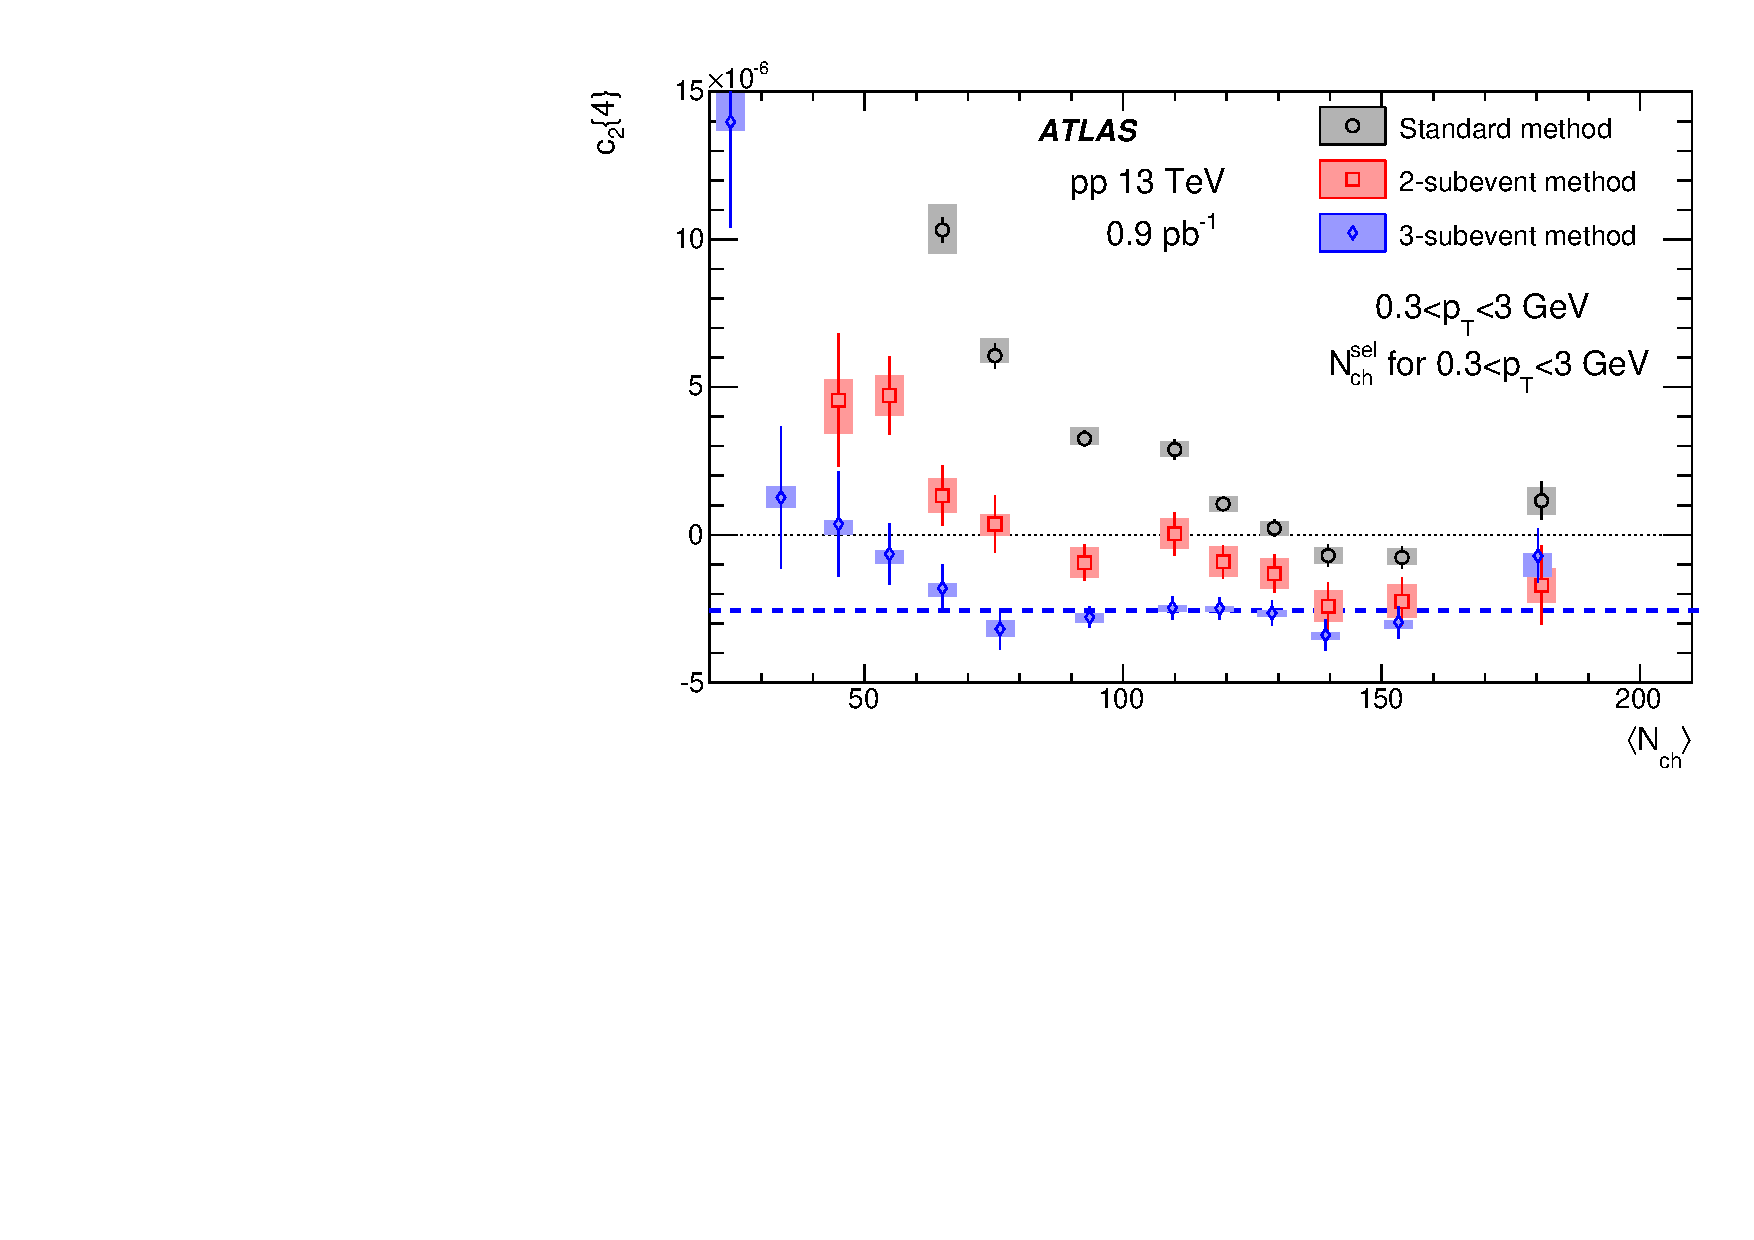
\includegraphics[width=.475\linewidth]{figs/chapter_subcumu/ATLAS_c24_pp13_pT0}
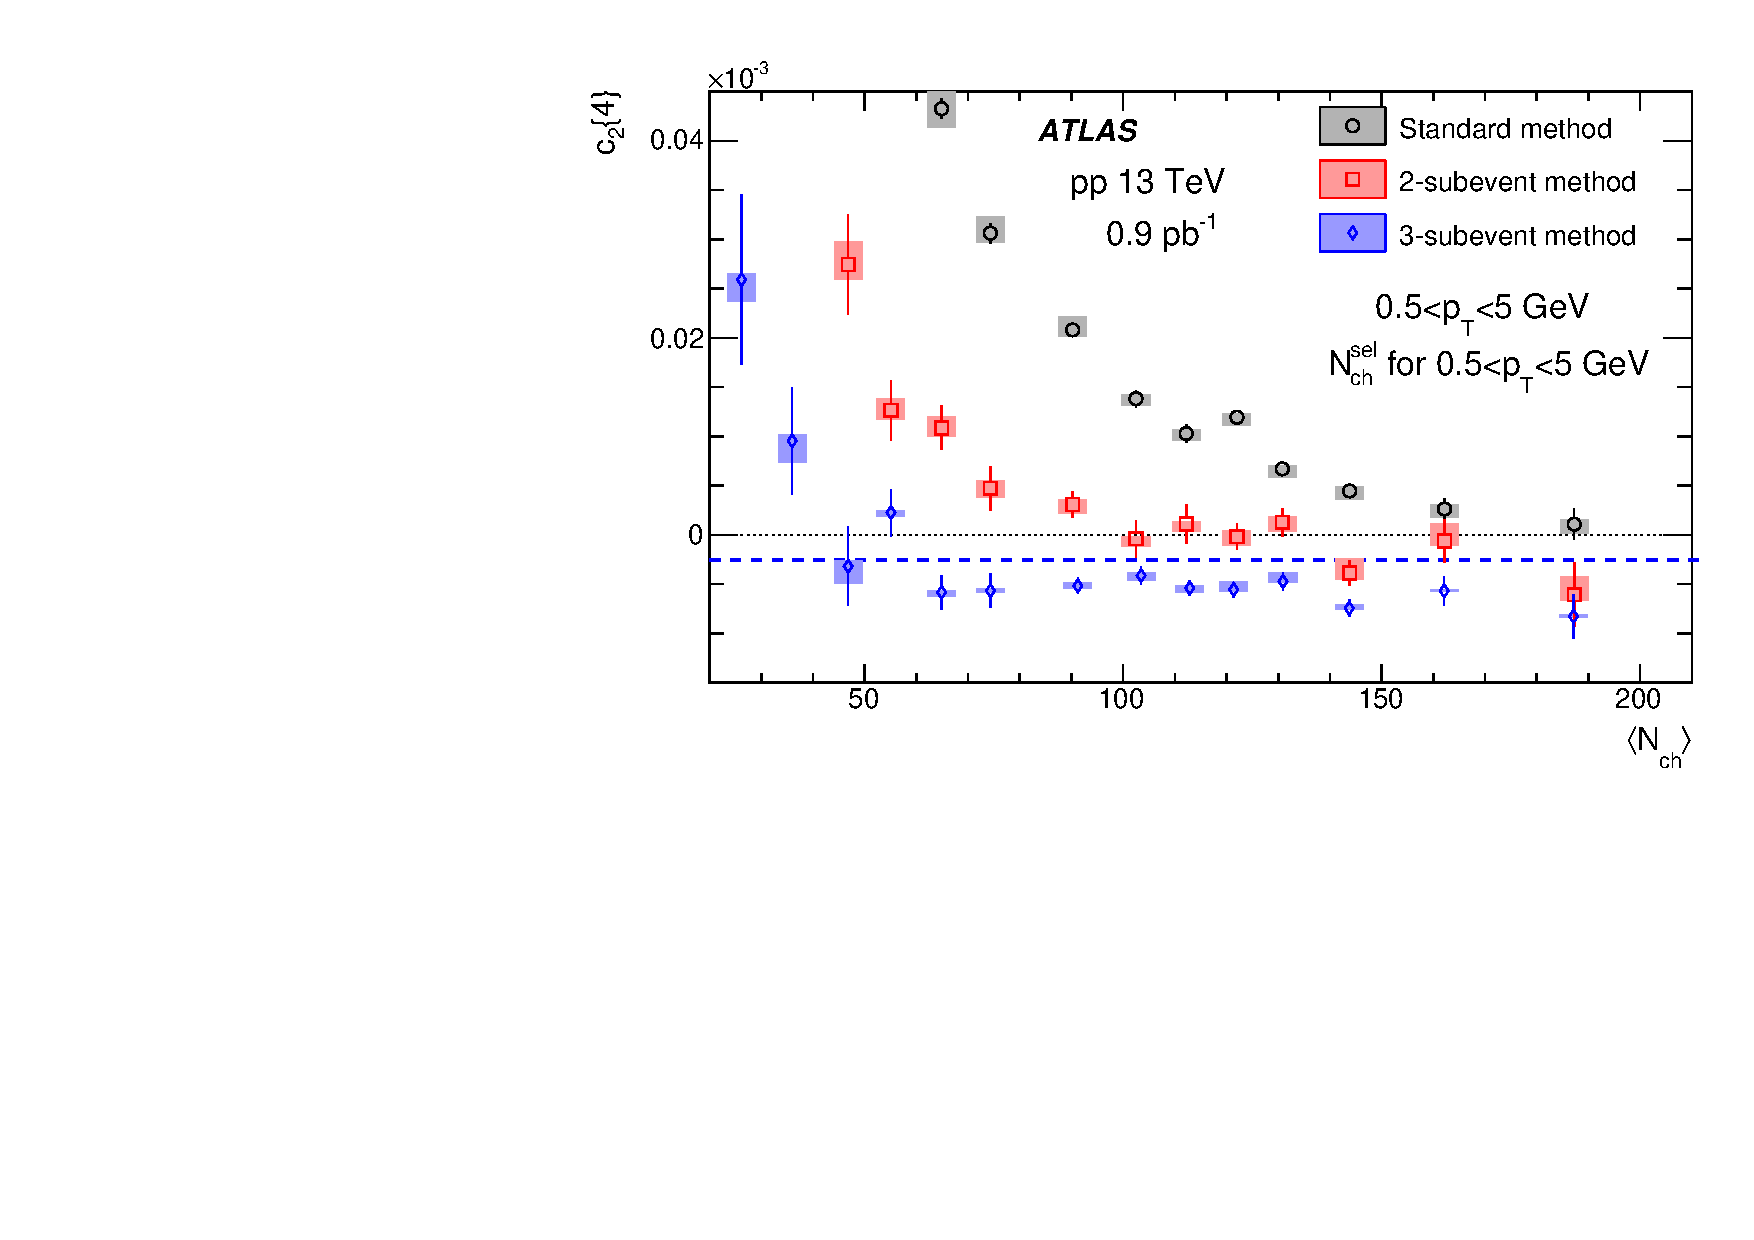
\includegraphics[width=.475\linewidth]{figs/chapter_subcumu/ATLAS_c24_pp13_pT1}
\caption{The $c_2\{4\}$ values calculated for charged particles with $0.3<\pT<3.0$ GeV (left) and $0.5<\pT<5.0$ GeV (right) compared for the three cumulant methods from the 13 TeV $pp$ data. The event averaging is performed for $\Nchsel$ calculated for the same $\pT$ range, which is then mapped to $\lr{\Nch}$, the average number of charged particles with $\pT>0.4$ GeV. The dashed line indicates the $c_2\{4\}$ value corresponding to a $4\%$ $v_2$ signal. The error bars and shaded boxes represent the statistical and systematic uncertainties, respectively.}
\label{fig:subcumu_ATLAS_c24_pp13}
\end{figure}

\begin{figure}[H]
\centering
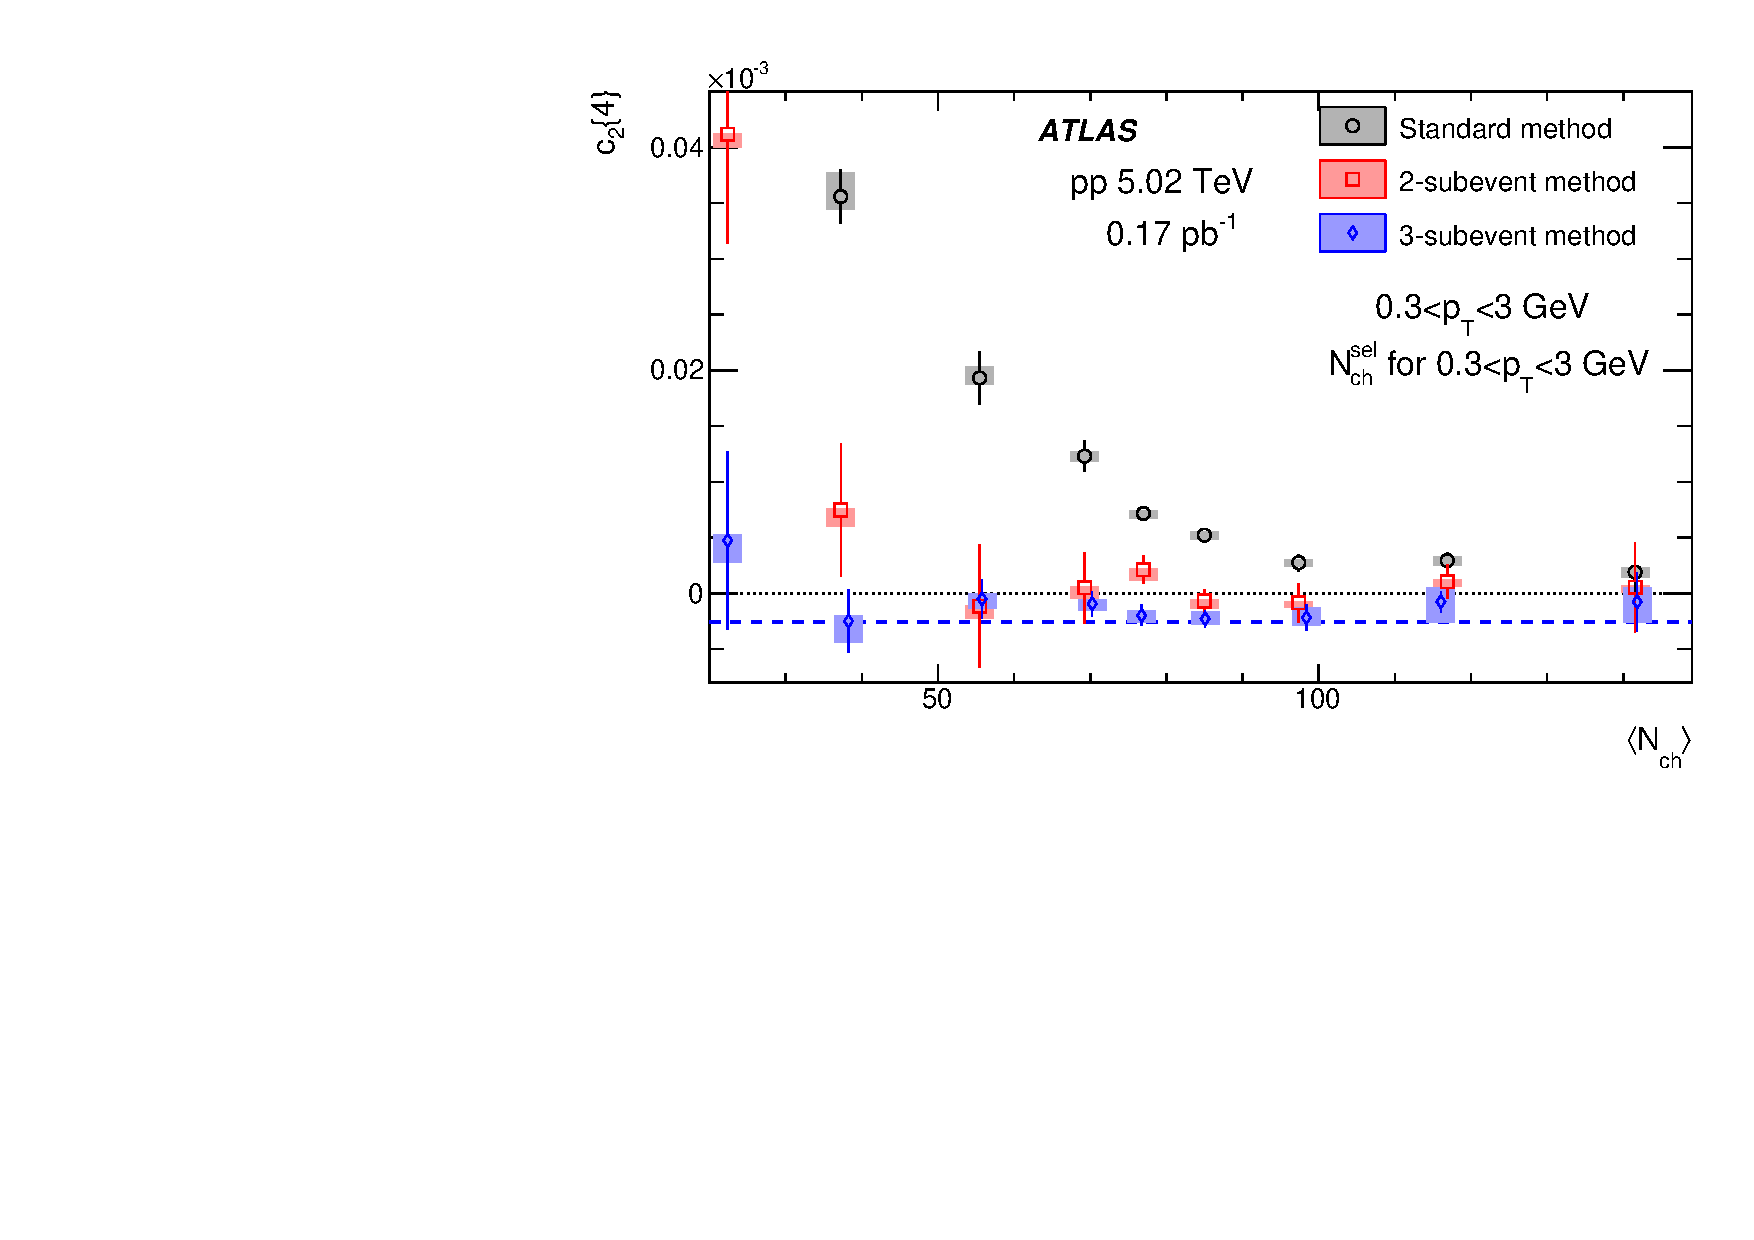
\includegraphics[width=.475\linewidth]{figs/chapter_subcumu/ATLAS_c24_pp5_pT0}
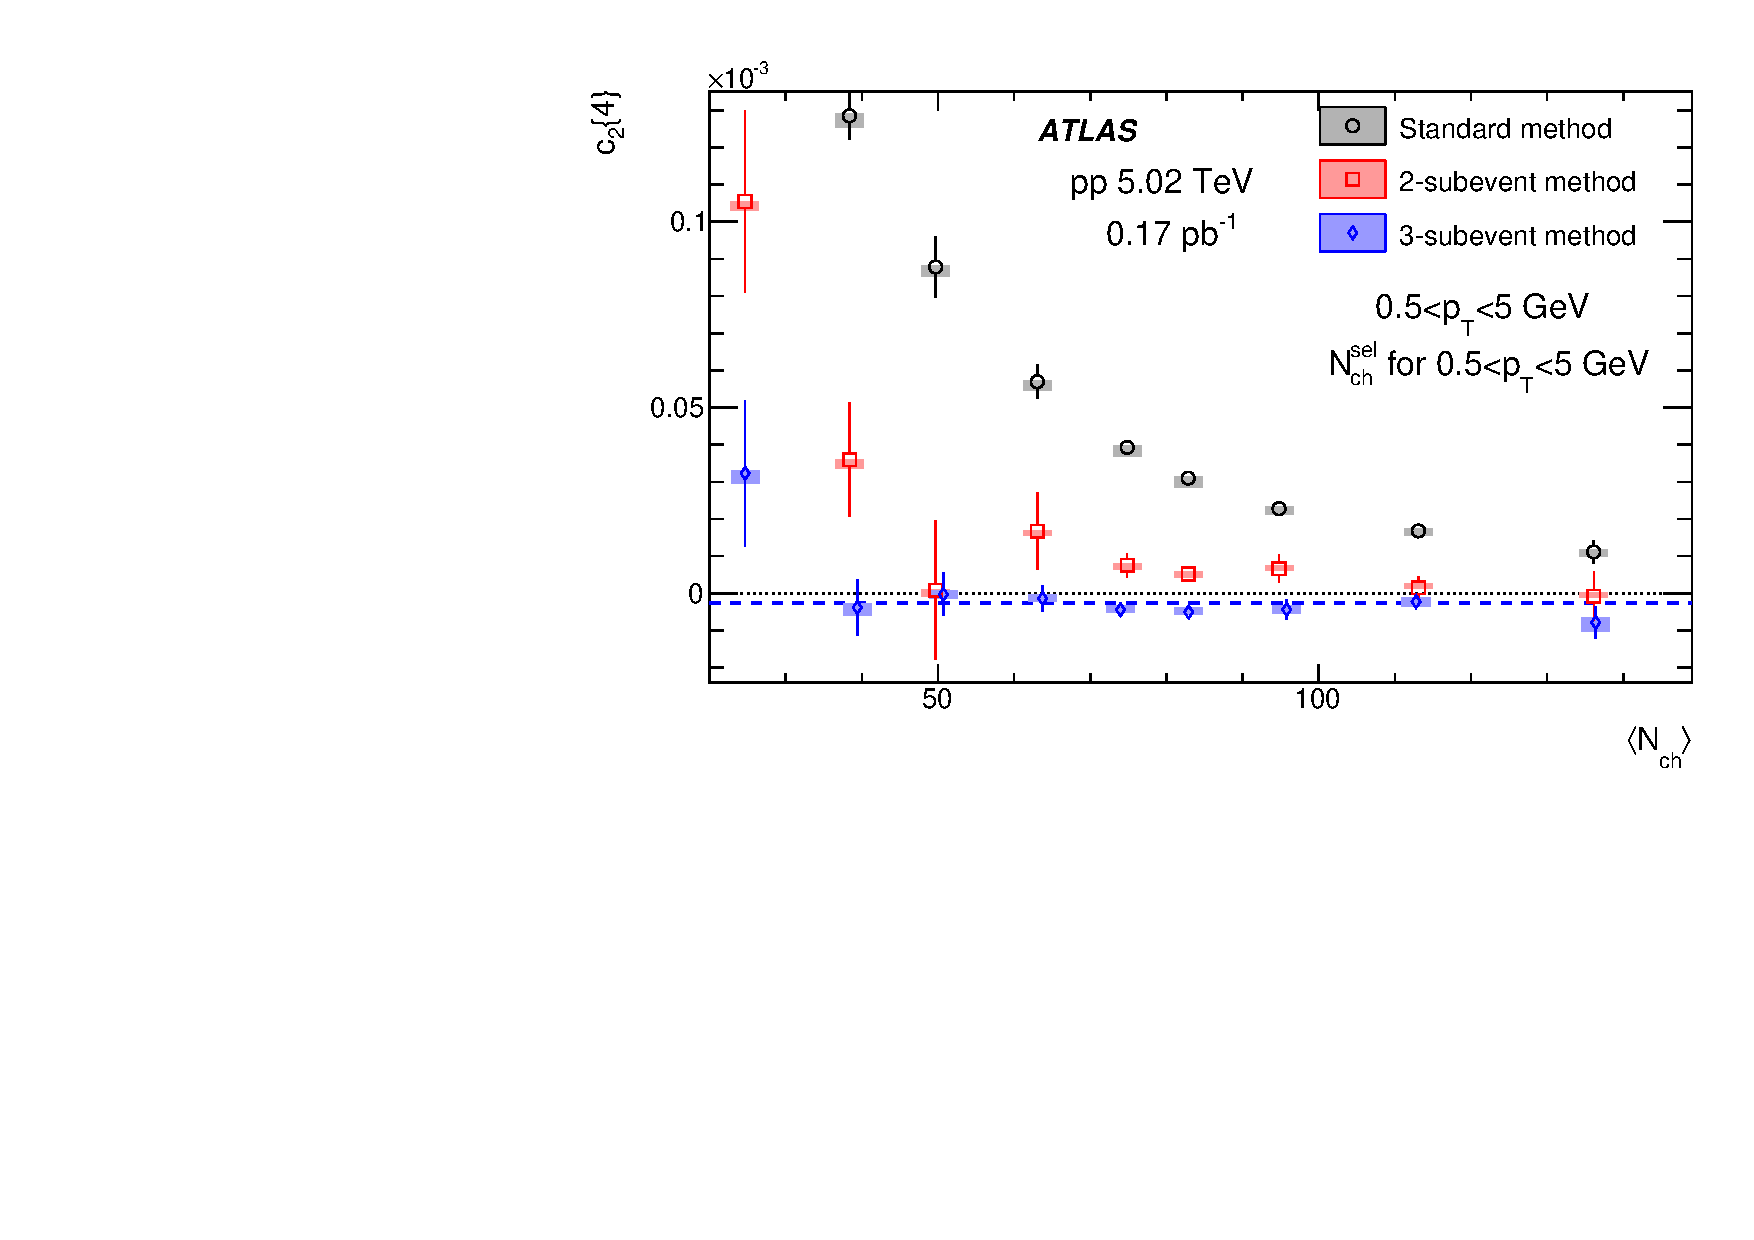
\includegraphics[width=.475\linewidth]{figs/chapter_subcumu/ATLAS_c24_pp5_pT1}
\caption{The $c_2\{4\}$ values calculated for charged particles with $0.3<\pT<3.0$ GeV (left) and $0.5<\pT<5.0$ GeV (right) compared for the three cumulant methods from the 5.02 TeV $pp$ data. The event averaging is performed for $\Nchsel$ calculated for the same $\pT$ range, which is then mapped to $\lr{\Nch}$, the average number of charged particles with $\pT>0.4$ GeV. The dashed line indicates the $c_2\{4\}$ value corresponding to a $4\%$ $v_2$ signal. The error bars and shaded boxes represent the statistical and systematic uncertainties, respectively.}
\label{fig:subcumu_ATLAS_c24_pp5}
\end{figure}

\begin{figure}[H]
\centering
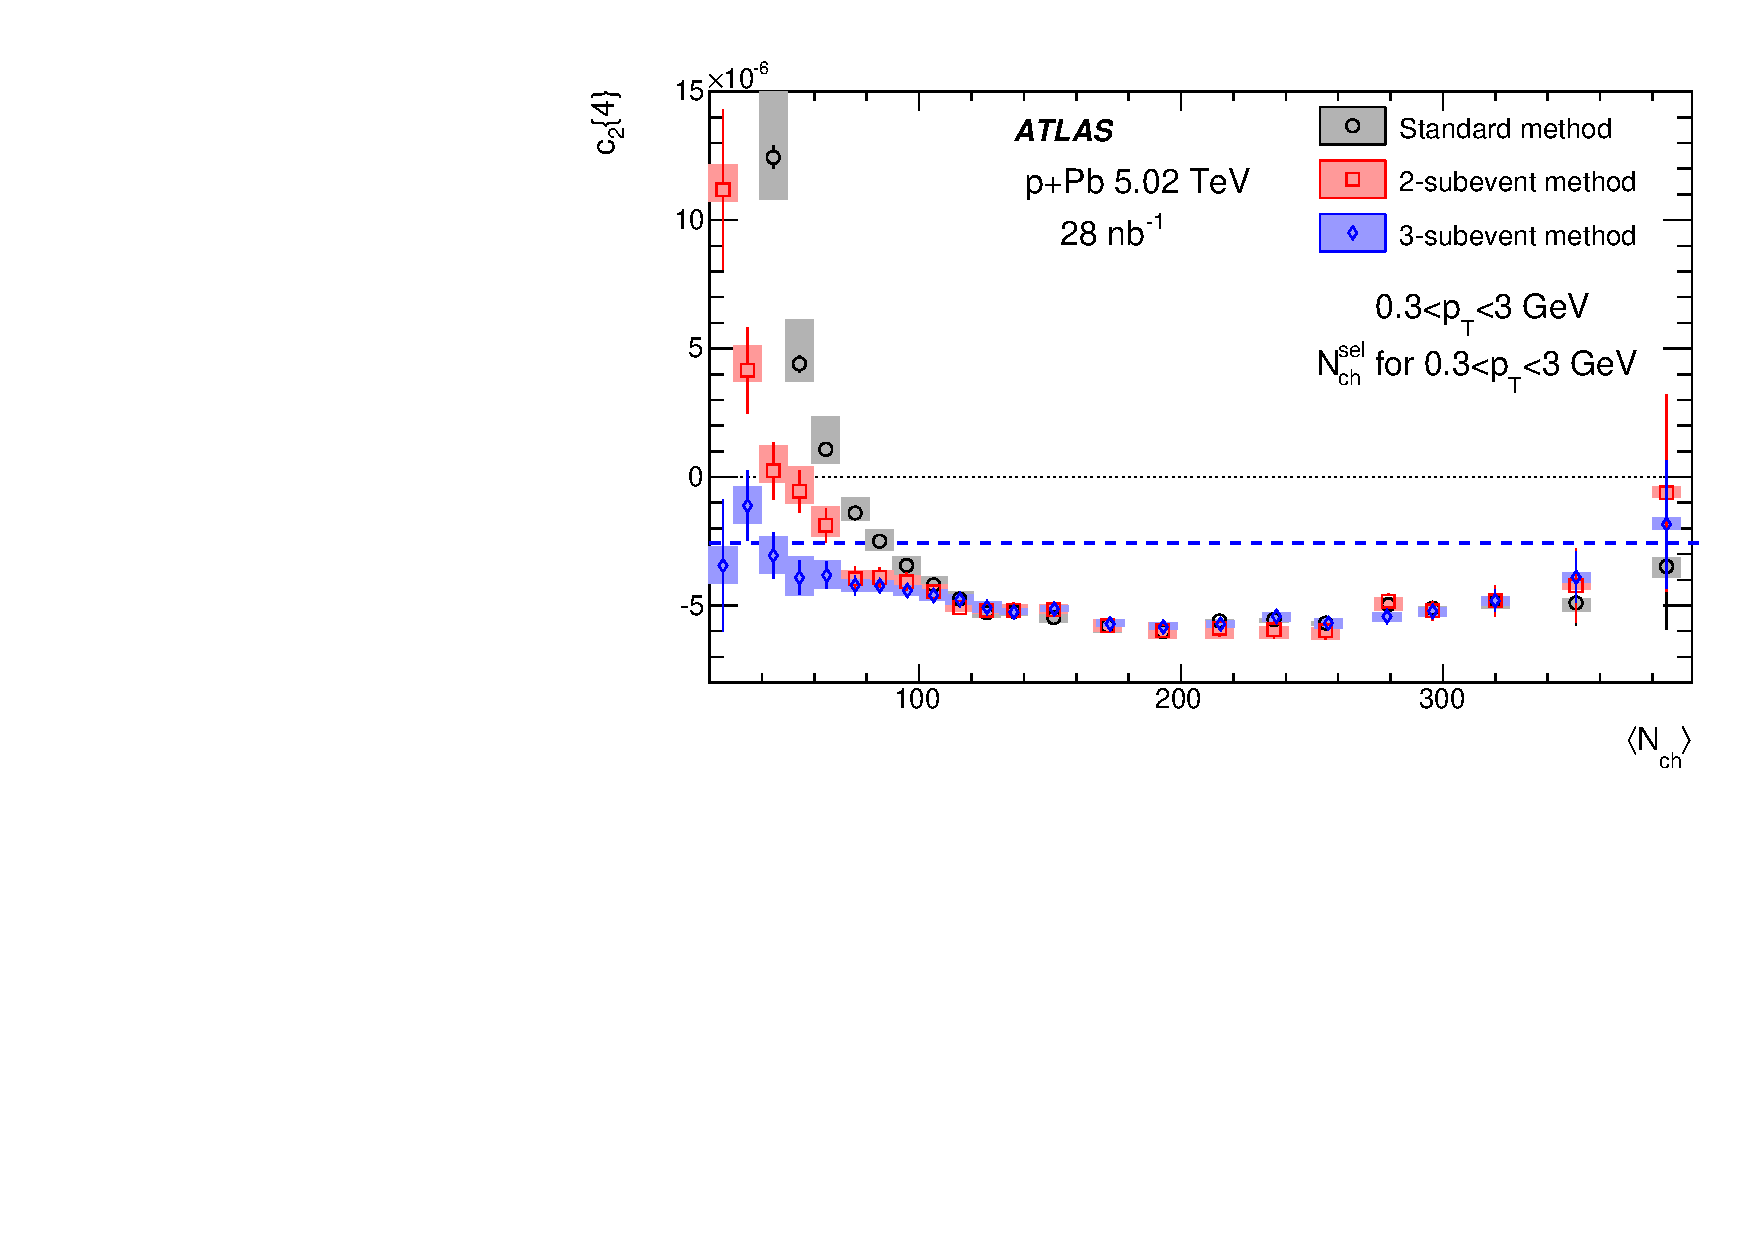
\includegraphics[width=.475\linewidth]{figs/chapter_subcumu/ATLAS_c24_pPb5_pT0}
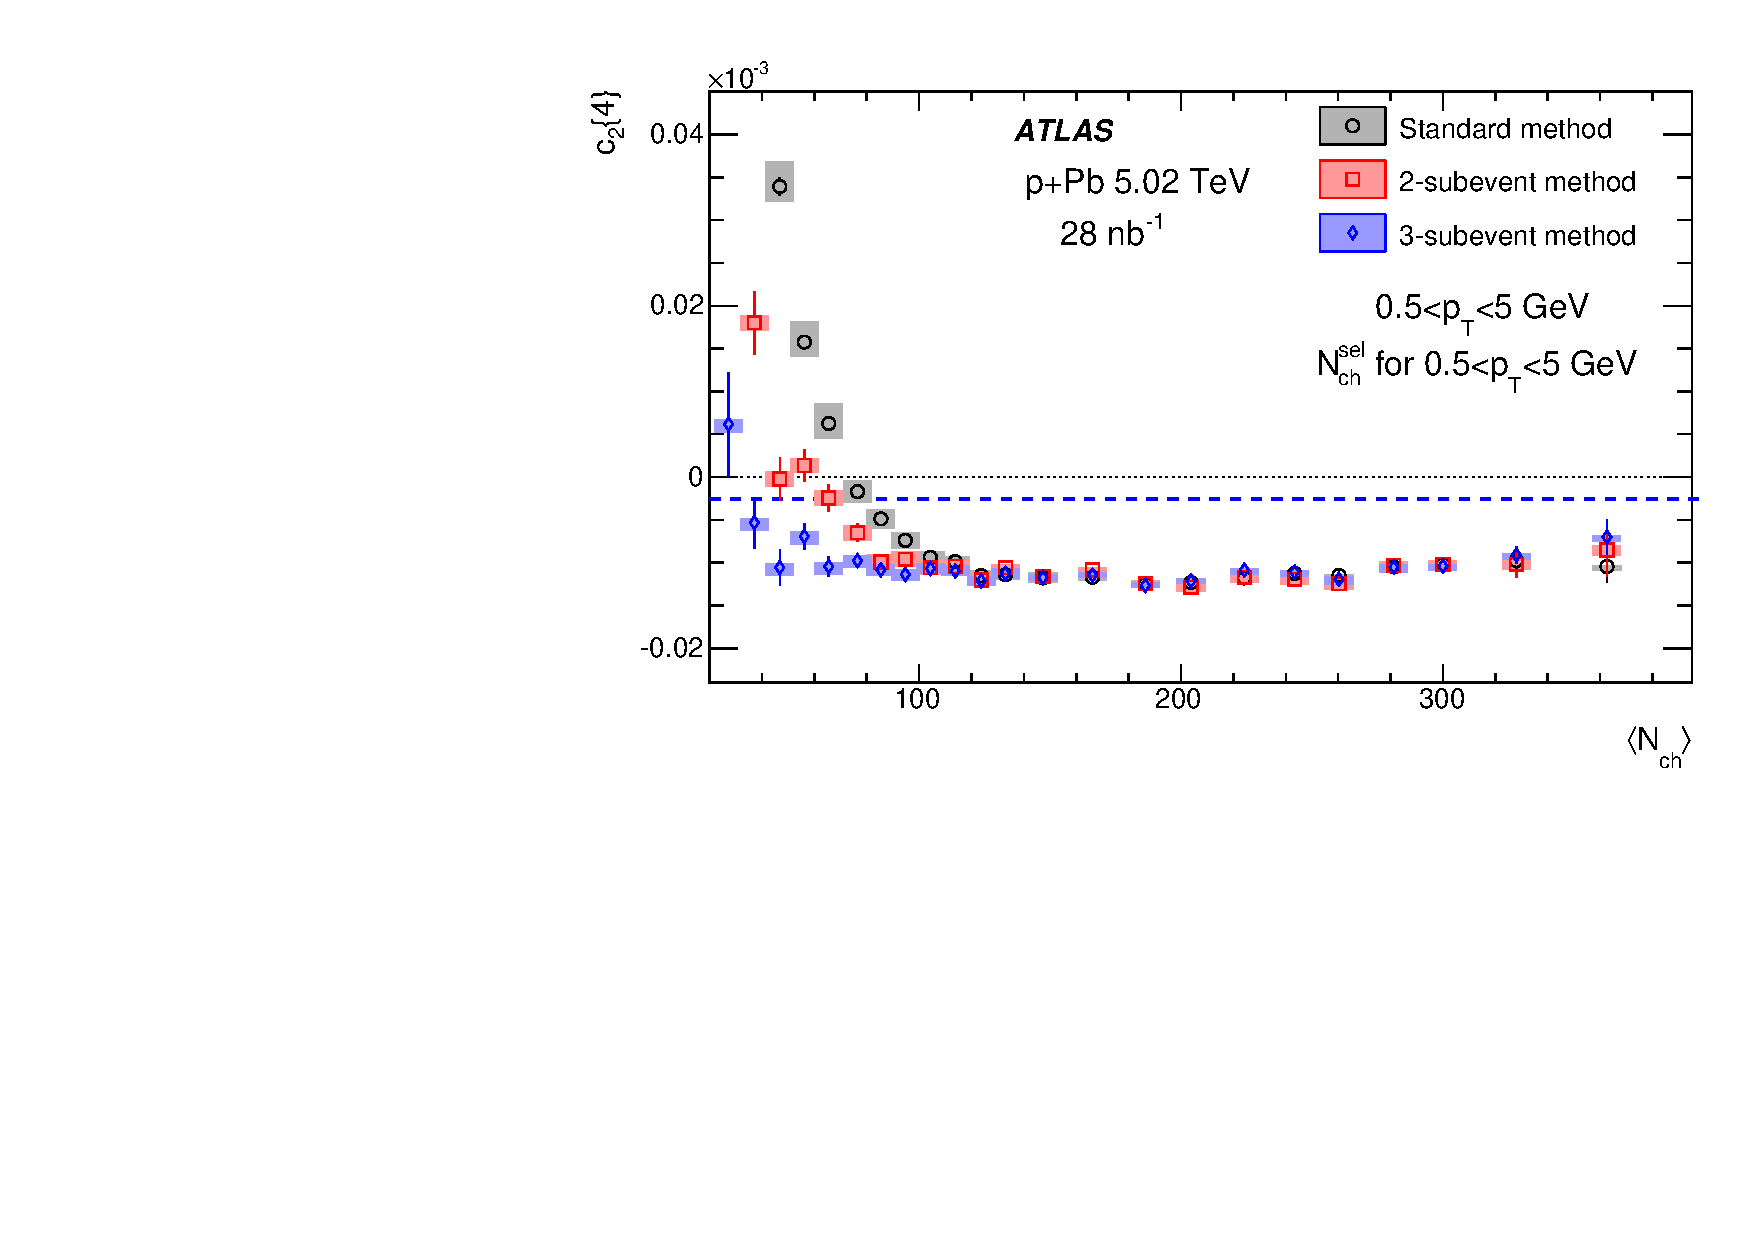
\includegraphics[width=.475\linewidth]{figs/chapter_subcumu/ATLAS_c24_pPb5_pT1}
\caption{The $c_2\{4\}$ values calculated for charged particles with $0.3<\pT<3.0$ GeV (left) and $0.5<\pT<5.0$ GeV (right) compared for the three cumulant methods from the 5.02 TeV $p$+Pb data. The event averaging is performed for $\Nchsel$ calculated for the same $\pT$ range, which is then mapped to $\lr{\Nch}$, the average number of charged particles with $\pT>0.4$ GeV. The dashed line indicates the $c_2\{4\}$ value corresponding to a $4\%$ $v_2$ signal. The error bars and shaded boxes represent the statistical and systematic uncertainties, respectively.}
\label{fig:subcumu_ATLAS_c24_pPb5}
\end{figure}

Figure~\ref{fig:subcumu_ATLAS_c34_pPb5} shows the $c_3\{4\}$ values from $p$+Pb collisions in the two $\pT$ ranges, obtained with the three-subevent method; they are zoomed-in so that statistical significance can be evaluated. Within their large statistical and systematic uncertainties, the values of $c_3\{4\}$ are systematically below zero, especially for $0.5<\pT<5.0$ GeV, where the $c_3\{4\}$ values are comparable to $-0.16\times 10^{-6}$, corresponding to a $v_3$ values of $2\%$ as indicated in the figure. The negative $c_3\{4\}$ values from the three-subevent method support the existence of long-range multi-particle triangular flow in $p$+Pb collisions. The $c_3\{4\}$ in $pp$ collisions are observed to be consistent with zero~\cite{Aaboud:2017blb}, more statistics are needed.

\begin{figure}[H]
\centering
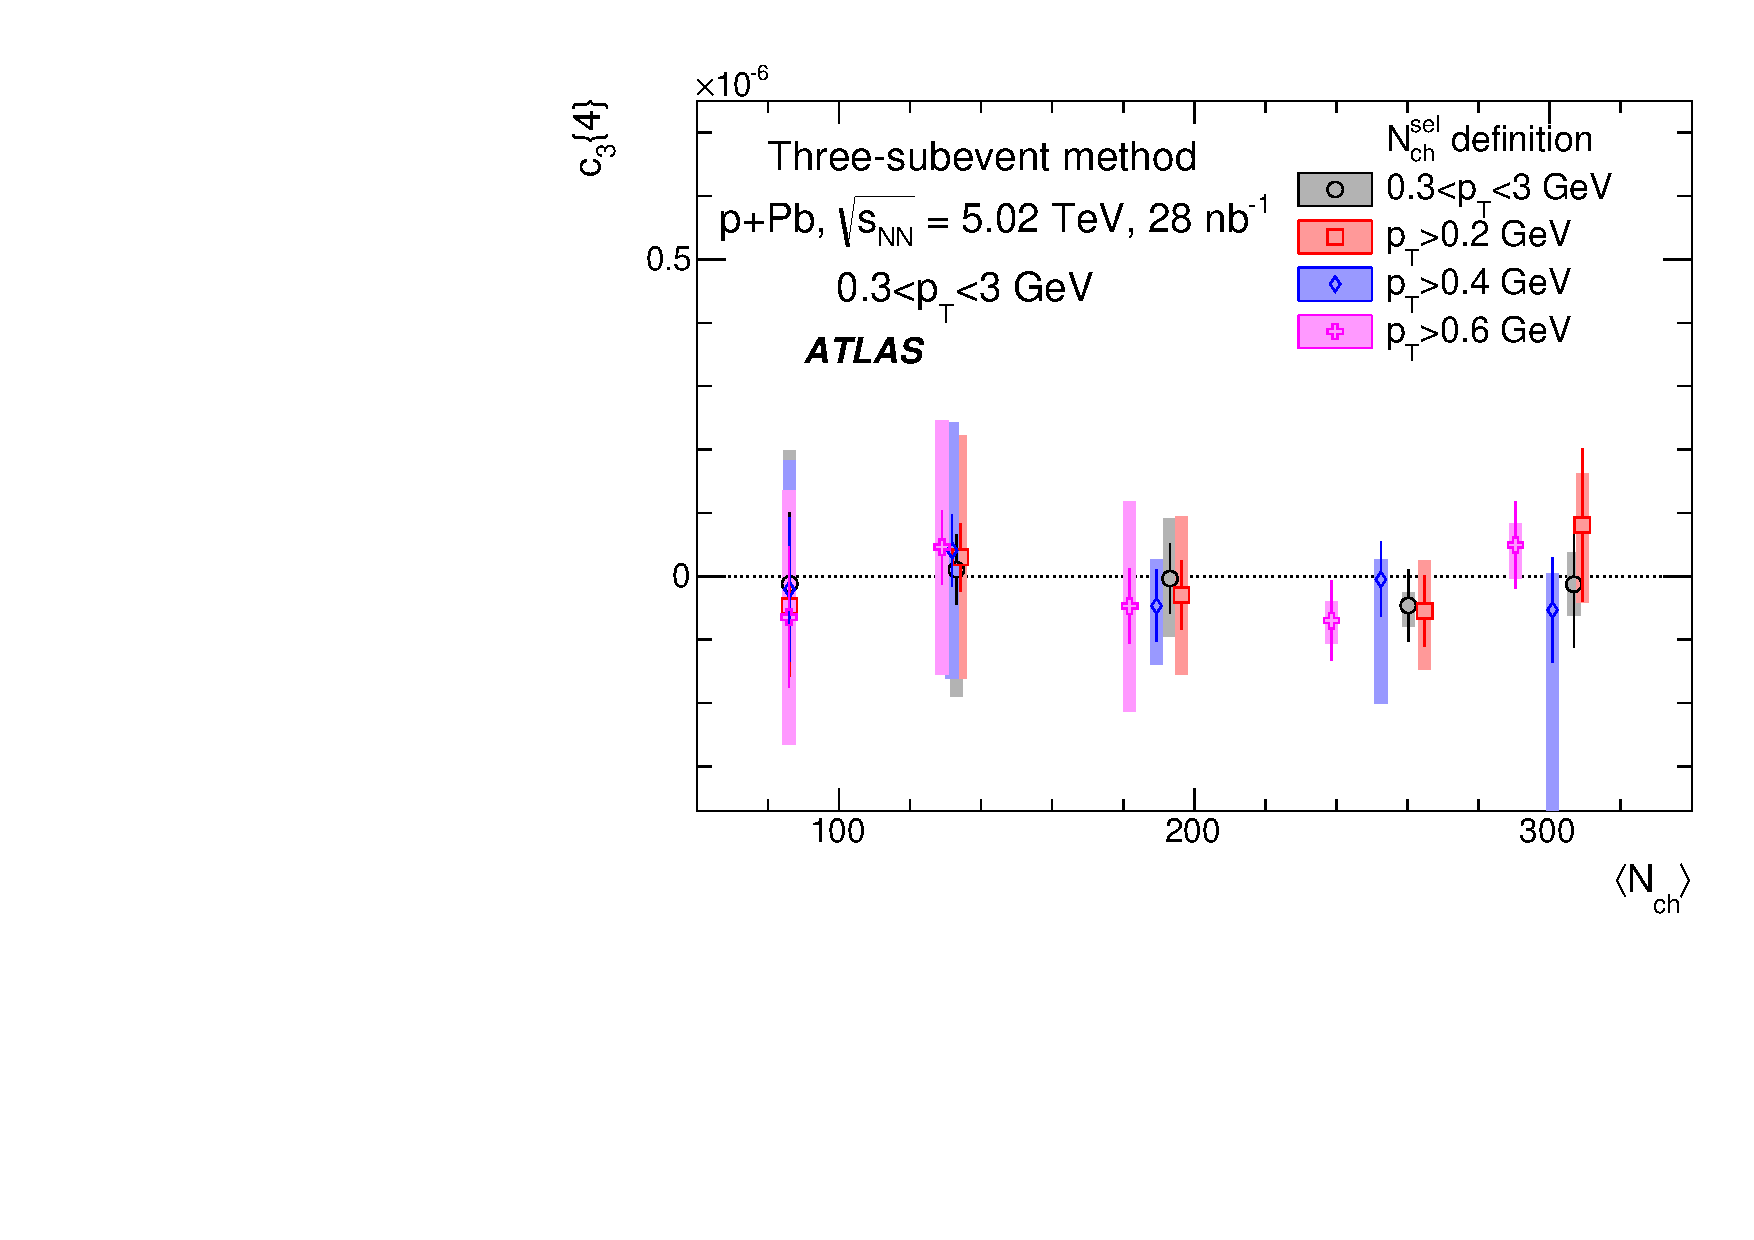
\includegraphics[width=.475\linewidth]{figs/chapter_subcumu/ATLAS_c34_pPb5_pT0}
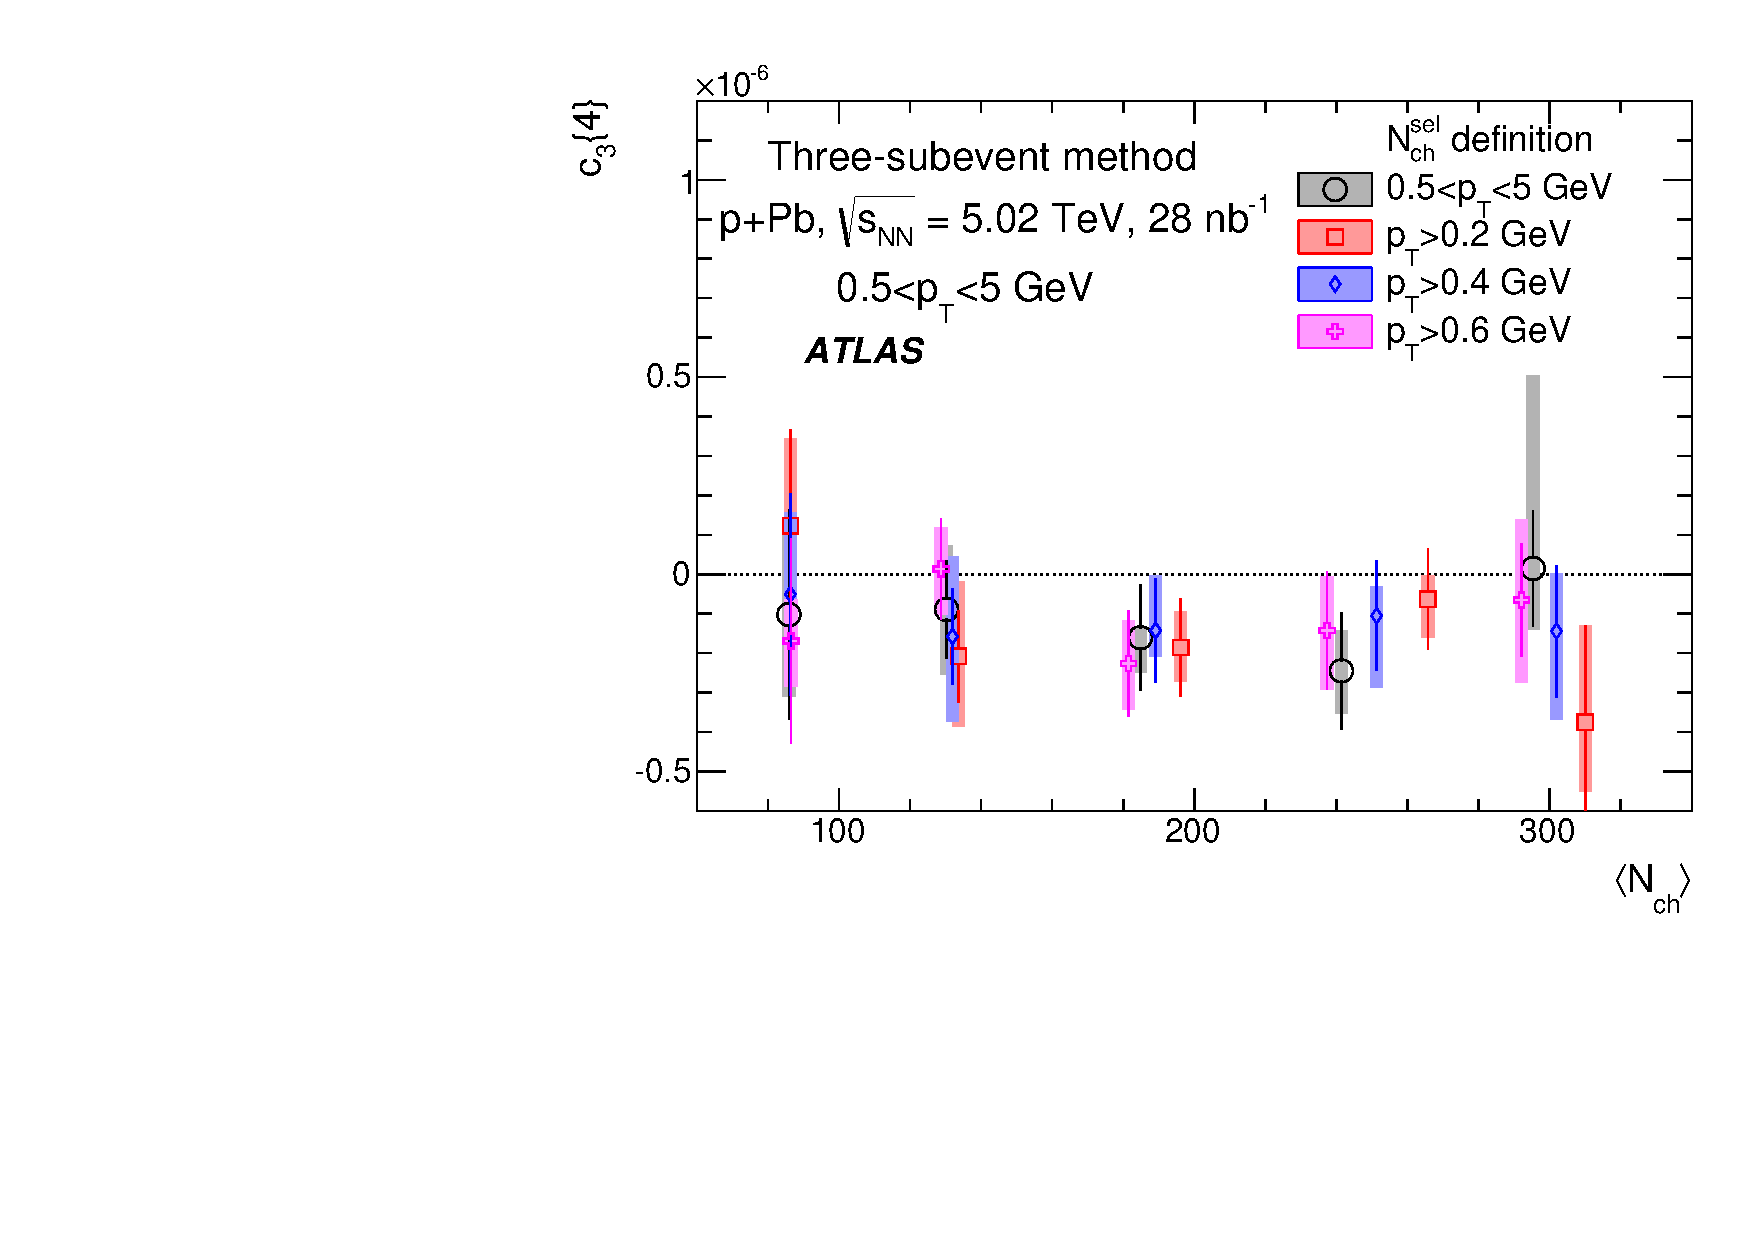
\includegraphics[width=.475\linewidth]{figs/chapter_subcumu/ATLAS_c34_pPb5_pT1}
\caption{The $c_3\{4\}$ values calculated for charged particles with $0.3<\pT<3.0$ GeV (left) and $0.5<\pT<5.0$ GeV (right) with the three-subevent cumulant method for the $p$+Pb data. The event averaging is performed for $\Nchsel$ calculated for the same $\pT$ range, which is then mapped to $\lr{\Nch}$, the average number of charged particles with $\pT>0.4$ GeV. The dashed line indicates the $c_3\{4\}$ value corresponding to a $2\%$ $v_3$ signal. The error bars and shaded boxes represent the statistical and systematic uncertainties, respectively.}
\label{fig:subcumu_ATLAS_c34_pPb5}
\end{figure}



\paragraph{Three-subevent flow harmonic $v_2\{4\}$}

The harmonic flow coefficients $v_2\{4\}$ can be obtained from the measured values of $c_2\{4\}$. Figure~\ref{fig:subcumu_ATLAS_v24_pT0} shows the $v_2\{4\}$ values for charged particles with $0.3<\pT<3.0$ GeV calculated using the three-subevent method in the three data sets. Results for the higher $\pT$ range ($0.5<\pT<5.0$ GeV) are presented in Figure~\ref{fig:subcumu_ATLAS_v24_pT1}. The value of $v_2\{4\}$ is measured down to $\lr{\Nch}\approx 50$ in $pp$ collisions and down to $\lr{\Nch}\approx 20-40$ in $p$+Pb collisions. The $v_2\{4\}$ values are observed to be approximately independent of $\lr{\Nch}$ in the measured range in the three data sets: $50<\lr{\Nch}<150$ for 5.02 TeV $pp$, $50<\lr{\Nch}<200$ for 13 TeV $pp$ and $20<\lr{\Nch}<380$ for 5.02 TeV $p$+Pb, respectively. Moreover, the $p$+Pb data suggest the value of $v_2\{4\}$ is slightly lower for $\lr{\Nch}>200$.

The values of $v_2\{4\}$ presented in Figures~\ref{fig:subcumu_ATLAS_v24_pT0} and \ref{fig:subcumu_ATLAS_v24_pT1} are also compared to the values of $v_2\{2\}$ obtained from the 2PC measurements~\cite{Aad:2014lta, Aaboud:2016yar} where the nonflow effects are estimated using low-multiplicity events ($\lr{\Nch}<20$) and then subtracted. The subtraction was performed either by a template fit, which includes the pedestal level from the $\lr{\Nch}<20$ events, or by a peripheral subtraction, which sets the pedestal level by a zero-yield at minimum (ZYAM) procedure~\cite{Adare:2008ae}. The peripheral subtraction explicitly assumes that the most peripheral events do not contain any long-range correlations~\cite{Aaboud:2016yar}, and so $v_2$ is forced to be zero at the corresponding $\lr{\Nch}$ value, which biases $v_2$ to a lower value in other multiplicity ranges.

\begin{figure}[H]
\centering
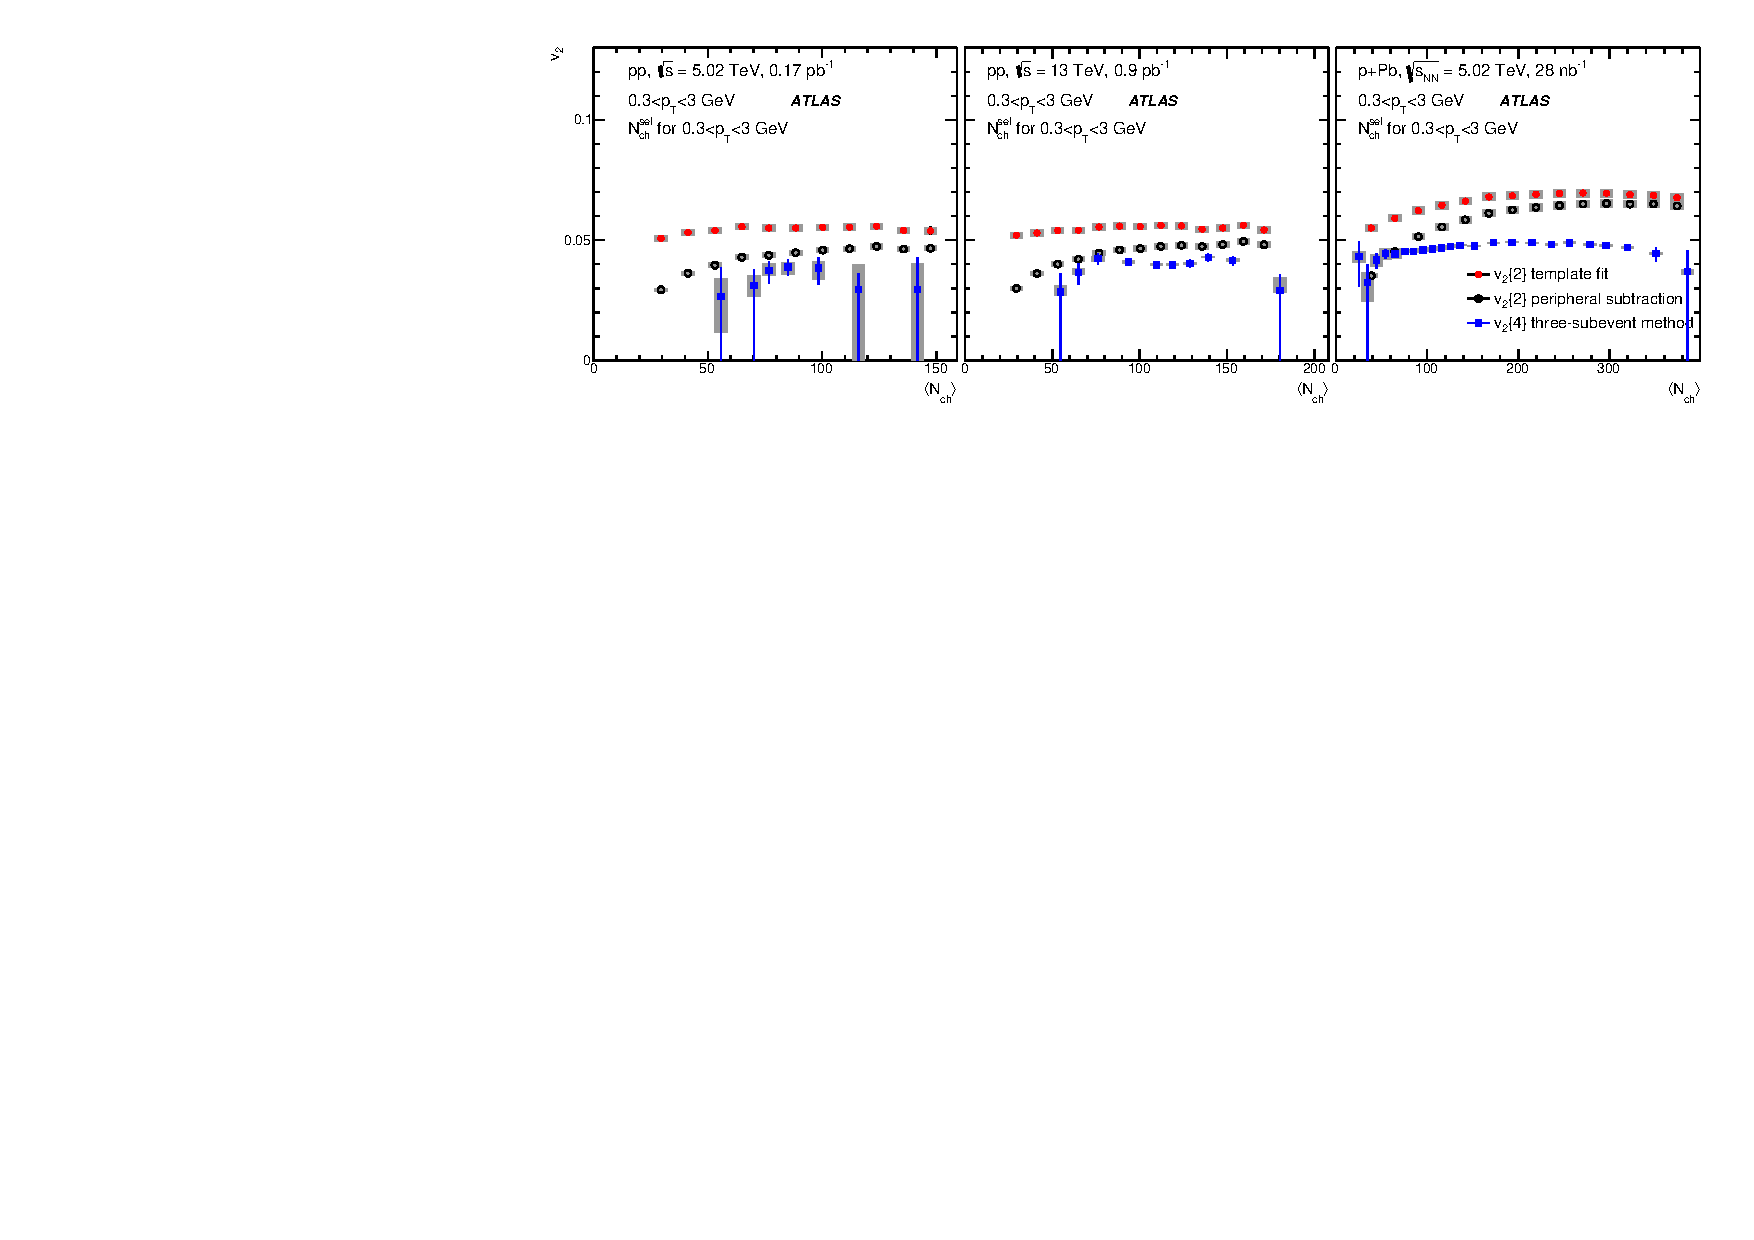
\includegraphics[width=.95\linewidth]{figs/chapter_subcumu/ATLAS_v24_pT0.pdf}
\caption{The $v_2\{4\}$ values calculated for charged particles with $0.3<\pT<3.0$ GeV using the three-subevent method in 5.02 TeV $pp$ (left), 13 TeV $pp$ (middle) and 5.02 TeV $p$+Pb collisions (right). They are compared to $v_2$ obtained from the 2PC analysis~\cite{Aad:2014lta, Aaboud:2016yar} where the nonflow effects are removed by a template fit procedure (solid circles) or with a fit after subtraction with a ZYAM assumption (peripheral subtraction, open circles). The error bars and shaded boxes represent the statistical and systematic uncertainties, respectively.}
\label{fig:subcumu_ATLAS_v24_pT0}
\end{figure}

\begin{figure}[H]
\centering
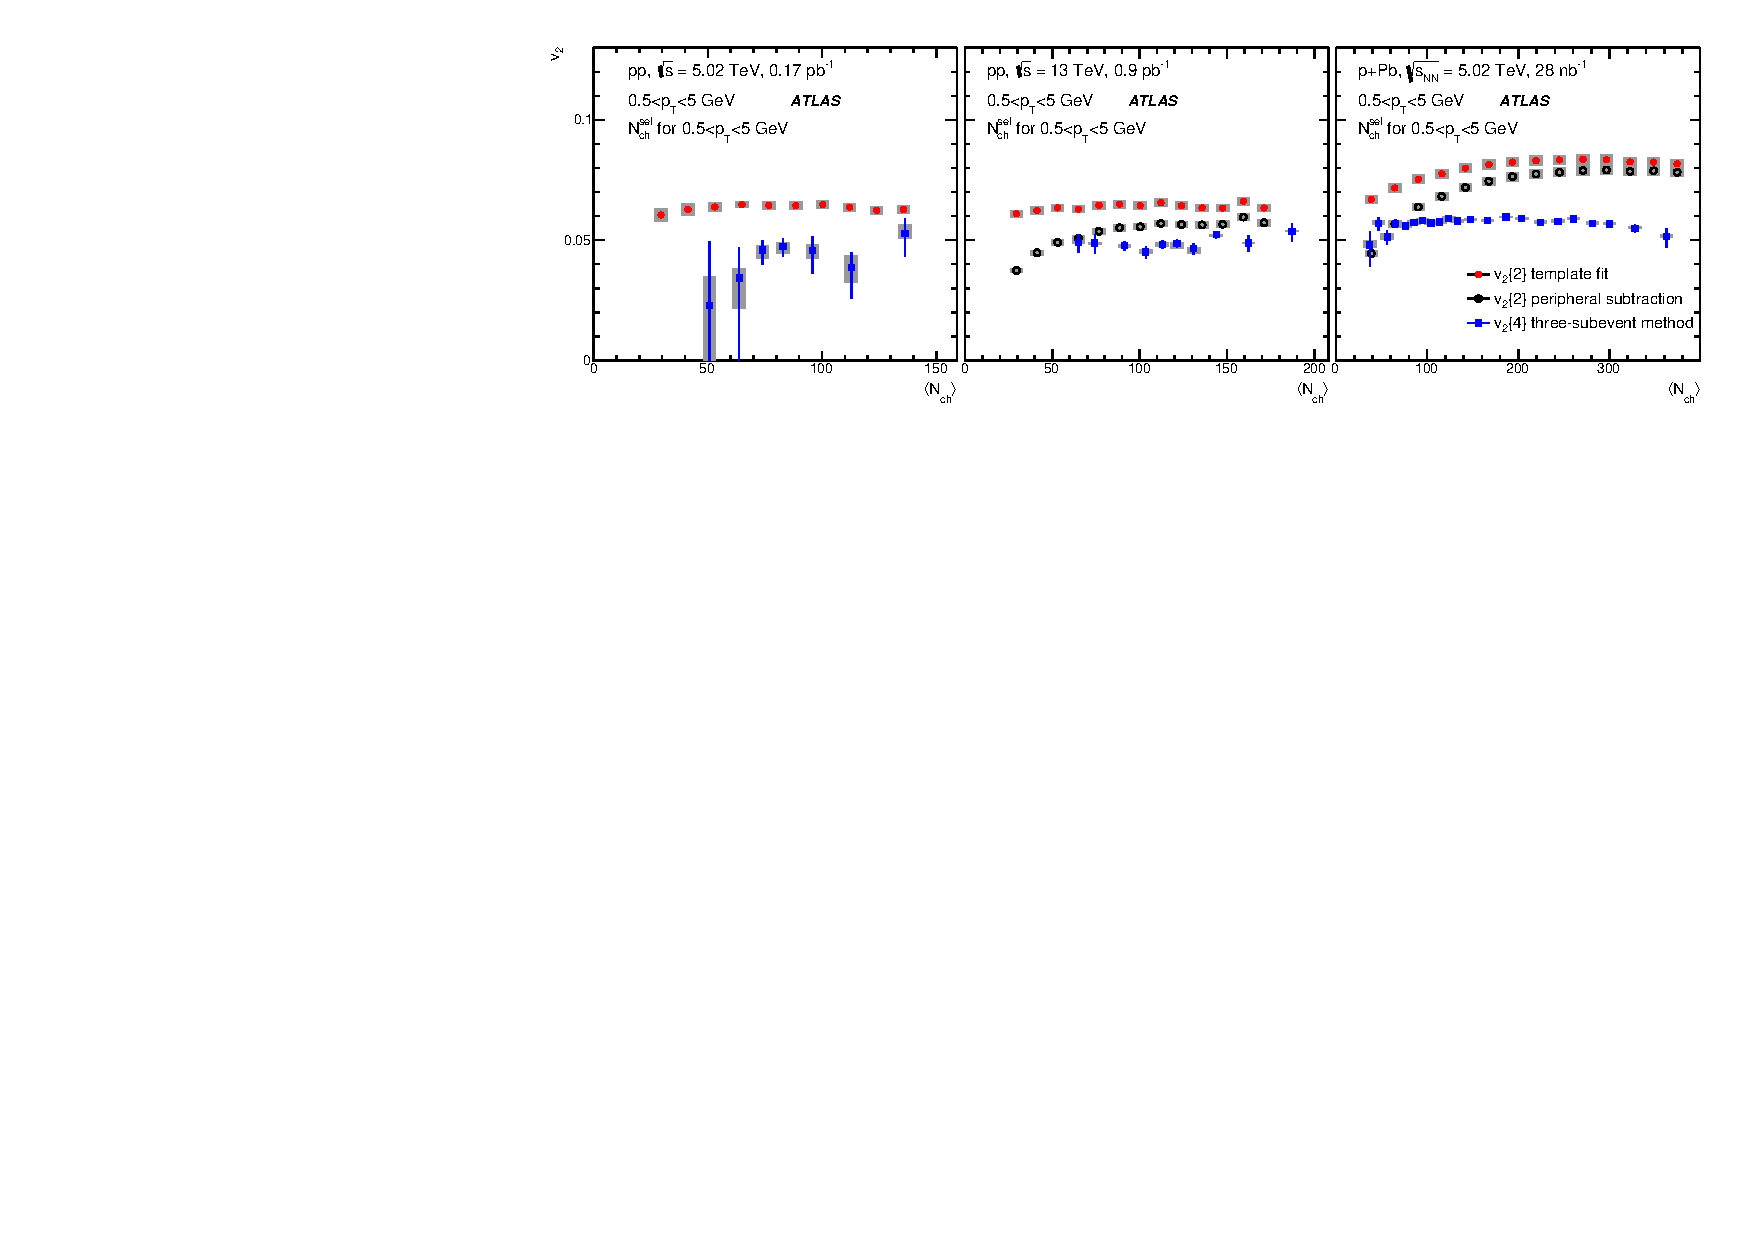
\includegraphics[width=.95\linewidth]{figs/chapter_subcumu/ATLAS_v24_pT1.pdf}
\caption{The $v_2\{4\}$ values calculated for charged particles with $0.5<\pT<5.0$ GeV using the three-subevent method in 5.02 TeV $pp$ (left), 13 TeV $pp$ (middle) and 5.02 TeV $p$+Pb collisions (right). They are compared to $v_2$ obtained from the 2PC analysis~\cite{Aad:2014lta, Aaboud:2016yar} where the nonflow effects are removed by a template fit procedure (solid circles) or with a fit after subtraction with a ZYAM assumption (peripheral subtraction, open circles). The error bars and shaded boxes represent the statistical and systematic uncertainties, respectively.}
\label{fig:subcumu_ATLAS_v24_pT1}
\end{figure}



\paragraph{Dependence on the number of sources in the initial state}

Figures~\ref{fig:subcumu_ATLAS_v24_pT0} and \ref{fig:subcumu_ATLAS_v24_pT1} show that the $v_2\{4\}$ values are smaller than the $v_2\{2\}$ values extracted using the template-fit method in both the $pp$ and $p$+Pb collisions. In various hydrodynamic models for small collision systems~\cite{Bzdak:2013rya, Yan:2013laa}, this difference can be interpreted as the influence of event-by-event flow fluctuations associated with the initial state, which is closely related to the effective number of sources $N_s$ for particle production in the transverse density distribution of the initial state~\cite{Yan:2013laa}:
\begin{equation}
\begin{split}
\frac{v_2\{4\}}{v_2\{2\}} &= [\frac{4}{3+N_s}]^{1/4} \\
N_s &= \frac{4v_2\{2\}^4}{v_2\{4\}^4}-3
\end{split}
\end{equation}

Figure~\ref{fig:subcumu_ATLAS_Ns} shows the extracted values of $N_s$ as a function of $\lr{\Nch}$ in 13 TeV $pp$ and 5.02 TeV $p$+Pb collisions, estimated using charged particles with $0.3<\pT<3.0$ GeV and $0.5<\pT<5.0$ GeV. It is observed that the $N_s$ value increases with $\lr{\Nch}$ in $p$+Pb collisions, reaching $N_s\sim 20$ in the highest multiplicity class, and it is consistent between the two $\pT$ ranges.

\begin{figure}[H]
\centering
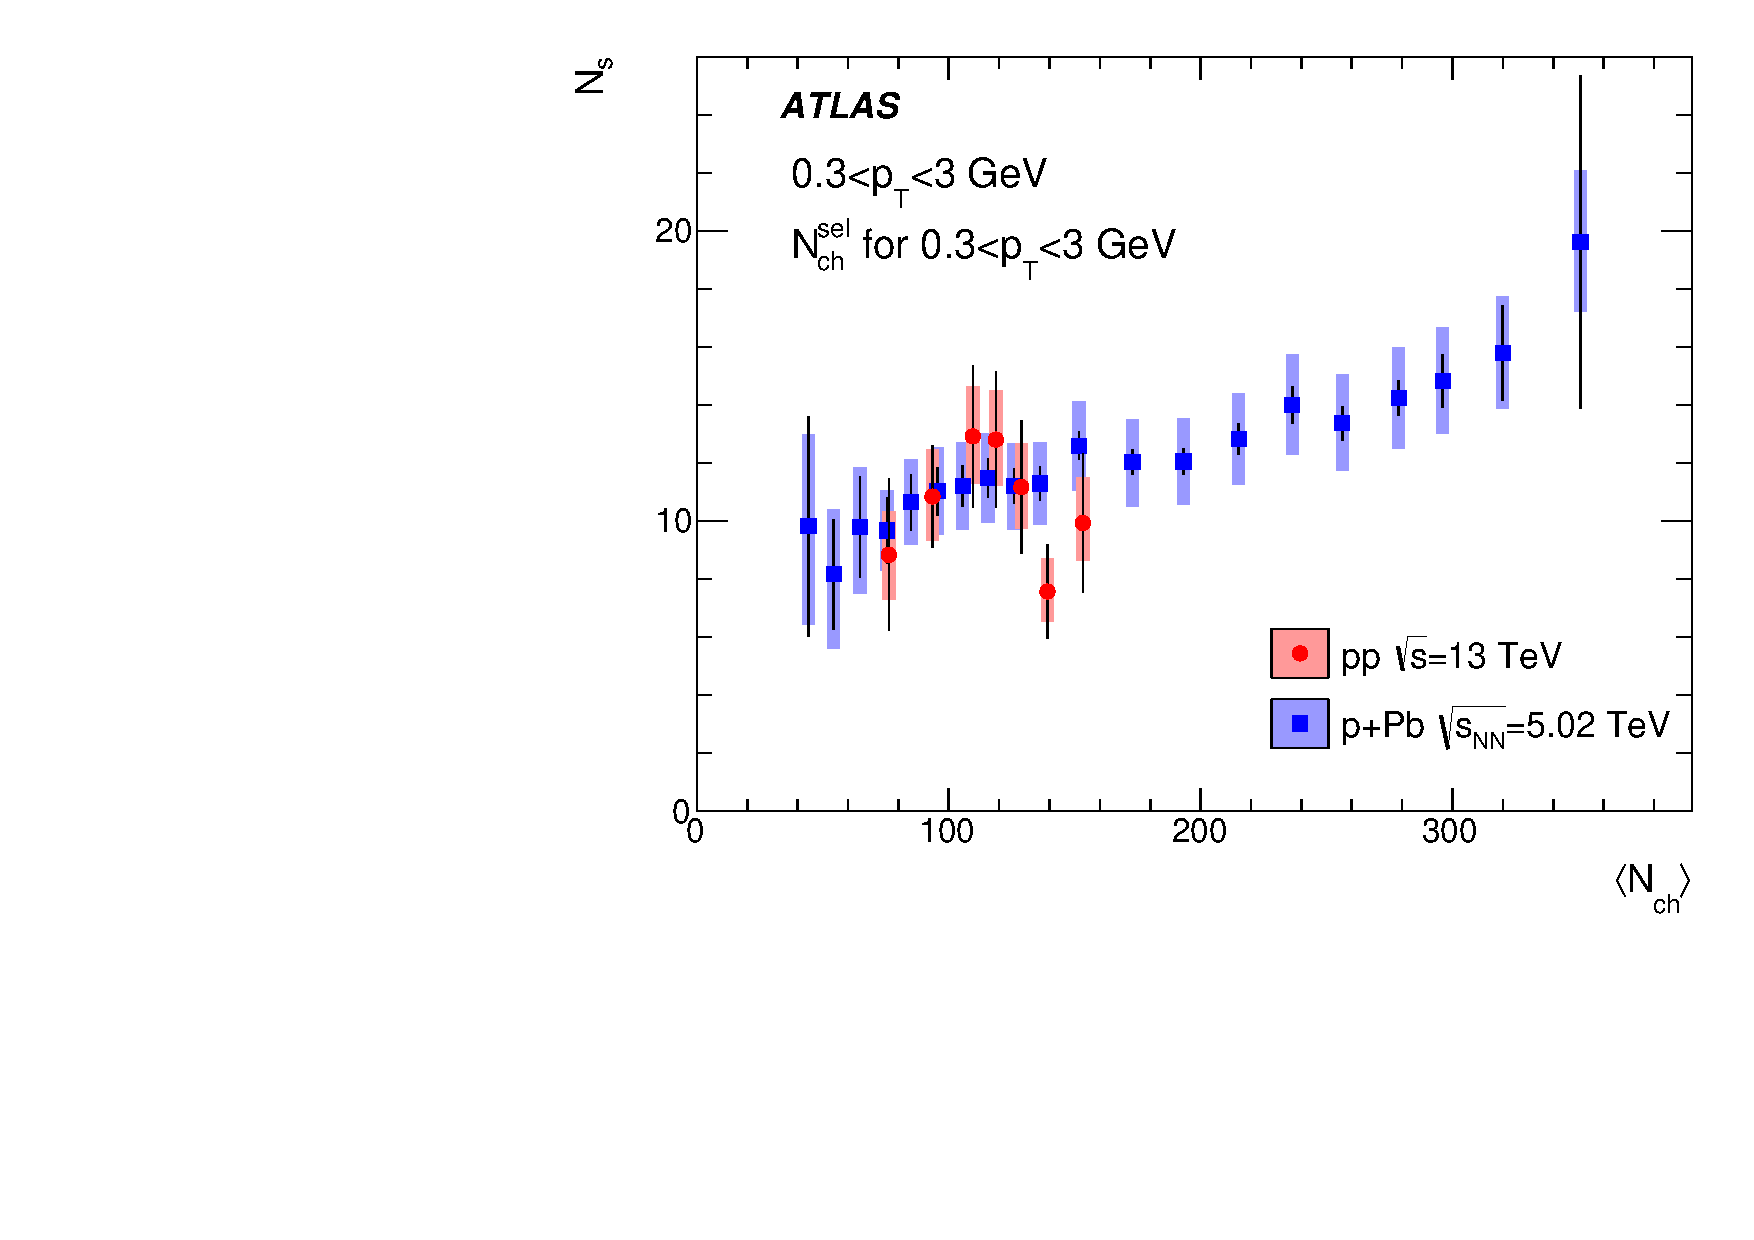
\includegraphics[width=.475\linewidth]{figs/chapter_subcumu/ATLAS_Ns_pT0.pdf}
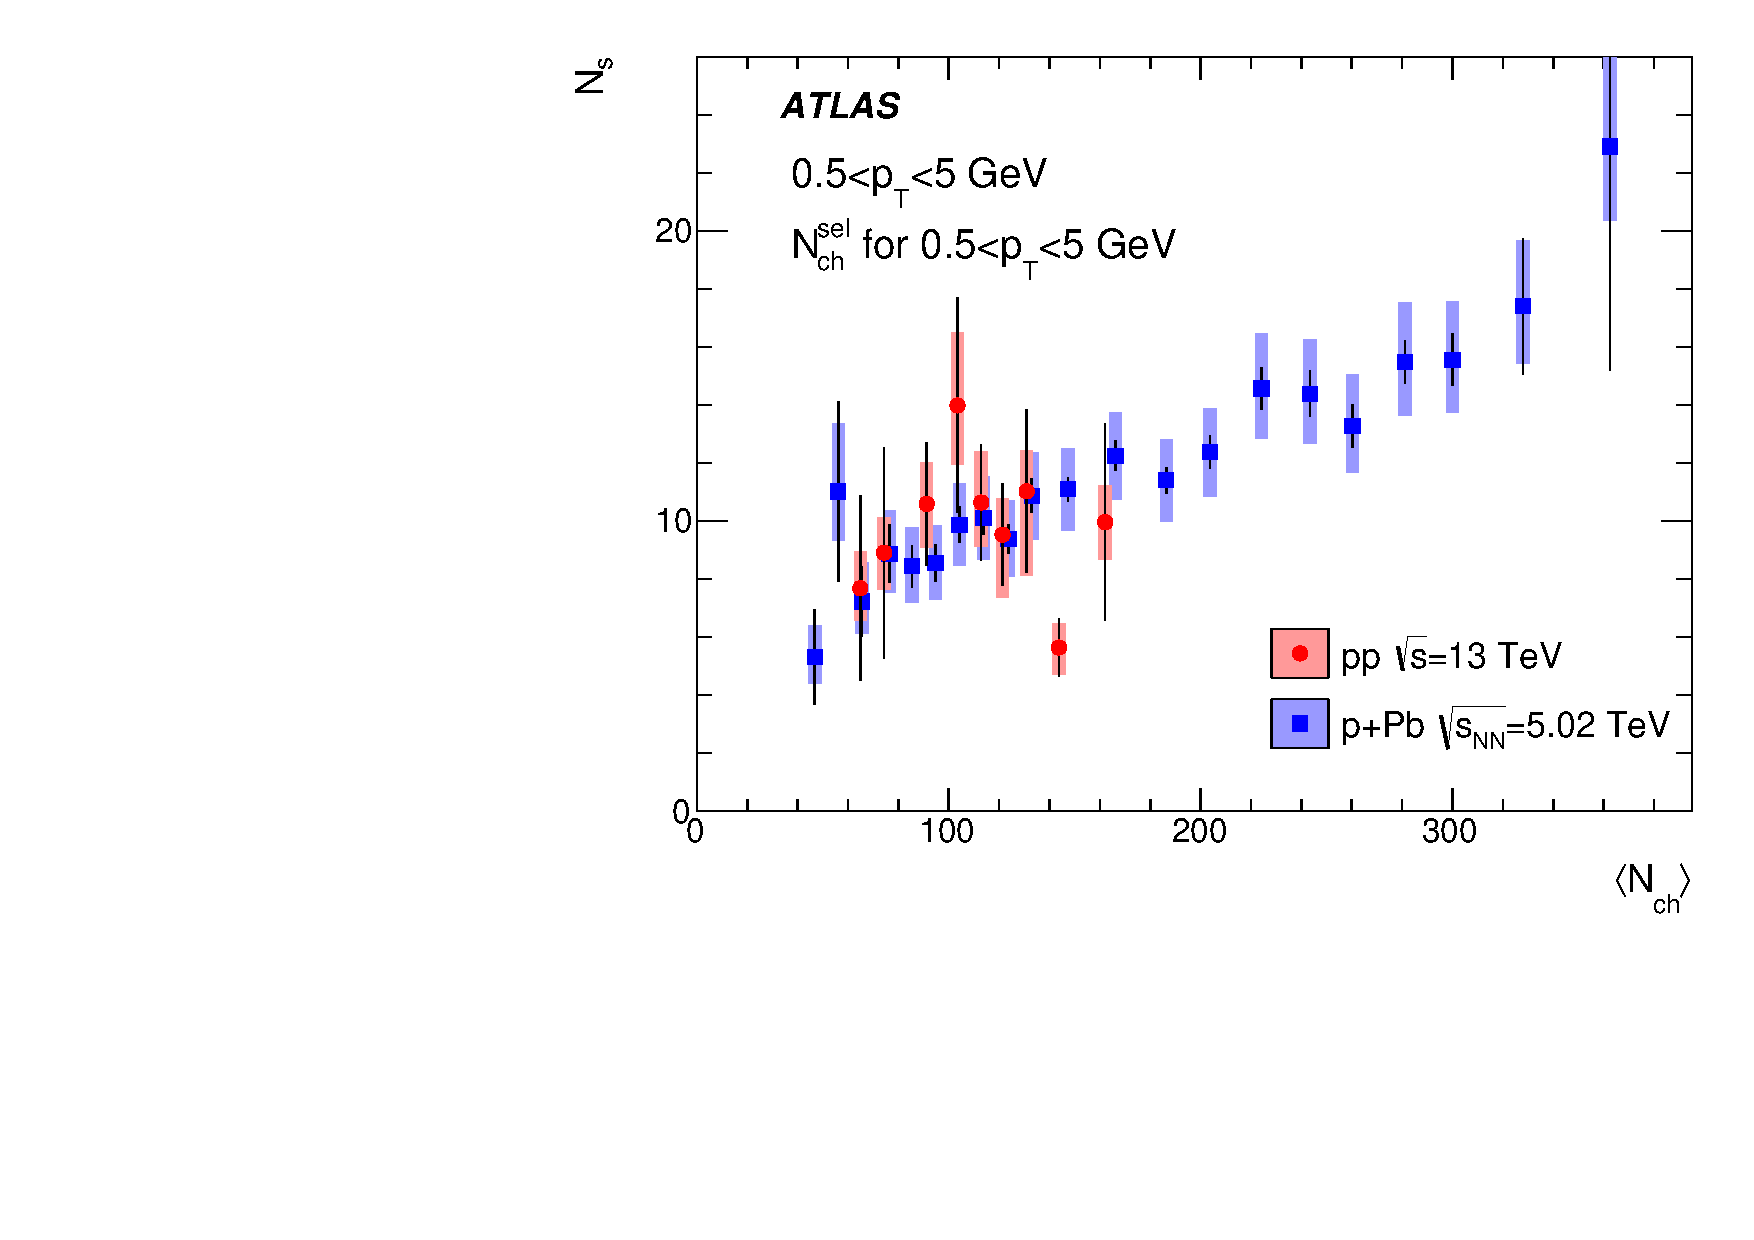
\includegraphics[width=.475\linewidth]{figs/chapter_subcumu/ATLAS_Ns_pT1.pdf}
\caption{The number of sources inferred from $v_2\{2\}$ and $v_2\{4\}$ measurements via the model framework in Refs.~\cite{Bzdak:2013rya, Yan:2013laa} in 13 TeV $pp$ and 5.02 TeV $p$+Pb collisions, for charged particles with $0.3<\pT<3.0$ GeV (left) and $0.5<\pT<5.0$ GeV (right). The error bars and shaded boxes represent the statistical and systematic uncertainties, respectively.}
\label{fig:subcumu_ATLAS_Ns}
\end{figure}

In the model framework in Refs.~\cite{Bzdak:2013rya, Yan:2013laa}, the values of $|c_2\{4\}|$ and $v_2\{4\}$ are expected to decrease for large $N_s$, which is compatible with the presented results. The slight decreases of $|c_2\{4\}|$ shown in Figure~\ref{fig:subcumu_ATLAS_c24_pPb5} for $p$+Pb collisions are compatible with the model predictions. The results for 13 TeV $pp$ collisions cover a limited $\lr{\Nch}$ range compared to $p$+Pb, but agree with $p$+Pb collisions in this range.



\subsection{Summary and discussion}

Ever since its discovery in small collision systems, the ridge phenomenon has been an area of insensitive study in the high-energy and heavy-ion physics community. The current debate is centered on the underlying multi-particle dynamics and collective nature of the long-range correlations, in particular whether the ridge is a global property of the event, and what is its connection to the collective flow in large collision systems~\cite{Dusling:2015gta, Schlichting:2016sqo}. The main challenge is to disentangle correlations involving all particles (flow or collectivity) from those involving a subset of the particles in restricted $\eta$ and $\phi$ space (nonflow). The 2PC method based on peripheral subtraction or the template fit method~\cite{Aad:2015gqa, Aaboud:2016yar, Aad:2014lta} can successfully remove the nonflow, but it does not address the multi-particle nature of the ridge. Results from multi-particle azimuthal cumulants, namely negative $c_n\{4\}$ and $c_n\{8\}$, positive $c_n\{6\}$, and the relation $v_n\{4\} \approx v_n\{6\} \approx v_n\{8\}$, has been used as a ``definition'' of collectivity~\cite{Khachatryan:2015waa, Khachatryan:2016txc}. However, this is true only if the flow fluctuations are relatively narrow or close to Gaussian and nonflow contributions to $c_n\{2k\}$ are small. ATLAS studies also shows that in $pp$ collisions the standard cumulant method is contaminated by nonflow correlations over the entire measured $\Nch$ range, which further complicates the relationship between different $v_n\{2k\}$s.

In this context, our studies address the issue of collectivity in small collision systems from two fronts: First, we clarify the statistical nature of multi-particle cumulants, and show that azimuthal cumulants are affected not only by the event-averaged flow and nonflow, but more importantly by the event-by-event fluctuations of flow and/or nonflow. We then propose alternative cumulant methods based on two or three subevents in non-overlapping $\eta$ ranges, and demonstrate that these methods can further suppress nonflow correlations.

The contribution of nonflow to cumulants can be discussed following a similar probabilistic approach. The contributions of flow and nonflow to cumulants are additive:
\begin{equation}
c_n\{2k\} = c_n\{2k, \text{flow}\} + c_n\{2k, \text{nonflow}\}
\end{equation}
The sign of $c_n\{2k,\text{nonflow}\}$ can be either positive or negative depending on the shape of event-by-event fluctuations of nonflow. The results from PYTHIA and ATLAS studies suggest that the value and sign of $c_n\{4\}$ in $pp$ collisions are driven mainly by the nonflow component in the standard cumulant method. The values of $c_n\{2k,\text{nonflow}\}$ are found to be very sensitive to the particle selection criteria used to define events for averaging.

Motivated by the discussions above, we have developed a cumulant method based on two or three $\eta$-separated subevents. The two-subevent method suppresses the nonflow from single jet fragmentation, while the three-subevent method also suppresses correlations between the two jets in a dijet. The performance of the two methods is quantified using PYTHIA simulation with only nonflow, as well as with physical flow added with an afterburner. The three-subevent method is shown to give consistent results between different criteria used to define event classes for averaging. The three-subevent method is able to recover flow signal as small as $4\%$ for $v_2$ for events with $\lr{\Nch}$  as low as 30.

We have applied subevent cumulant method to $pp$, $p$+Pb data, and the three-subevent method provides a measurement of $c_2\{4\}$ that is negative in all three data sets over a broad range of $\lr{\Nch}$. The magnitude of $c_2\{4\}$ increases with $\pT$ and is nearly independent of $\lr{\Nch}$ but in $p$+Pb collisions the values become smaller at high multiplicities. There results provide direct evidence for the presence of long-range multi-particle azimuthal correlations in broad $\lr{\Nch}$ ranges in $pp$ and $p$+Pb collisions, and these long-range multi-particle correlations persist even in events with rather low multiplicity of $\lr{\Nch}\sim 40$. The $c_3\{4\}$ values are consistent with zero in $pp$ collisions, but are systematically below zero in $p$+Pb collisions, compatible with the presence of significant long-range multi-particle triangular flow in $p$+Pb collisions. The single-particle harmonic coefficient $v_2\{4\}$ is calculated and compared with $v_2\{2\}$ obtained previously using the 2PC method, where the nonflow contributions were estimated and subtracted. The magnitude of $v_2\{4\}$ is smaller than that for $v_2\{2\}$, as expected for a long-range final-state hydrodynamic collective effect. The ratio of $v_2\{4\}$ to $v_2\{2\}$ is used, in a model-dependent framework, to infer the number of particle-emitting sources in the initial-state geometric configuration. The number of sources extracted within this framework is found to increase with $\lr{\Nch}$ in $p$+Pb collisions.

The subevent cumulant technique and the new results provide direct evidence that the ridge is indeed a long-range collective phenomenon involving many particles distributed across a broad rapidity interval. The subevent method also provides a strong test of the gluon saturation models used to describe $c_2\{4\}$ obtained with the standard cumulant method, where it was argued that the sign change of $c_2\{4\}$ could be due to non-Gaussian correlations of the domains of strong QCD fields in the initial state~\cite{Dumitru:2014yza, Lappi:2015vta}. It would be interesting to see whether or not such color domains can simultaneously correlated three or more pseudorapidity ranges and contribute to subevent cumulants.



\subsection{Outlook}

\subsubsection{Potential improvements}

Looking into the future, there are several potential improvements of the subevent cumulant method:
\begin{itemize}
\item Rapidity gap between subevents. This can further suppress nonflow sources falling on the boundary between subevents. Furthermore, by requiring the same rapidity gap as in 2PC analysis, $v_n\{4\}$ can be compared directly with $v_n\{2\}$.
\item Four or higher number of subevents. This can further reduce nonflow and prove that the azimuthal collectivity indeed exists between particles in four or more distinct $\eta$ ranges. But this also reduces statistical significance.
\item Subevent defined by nonflow. For example, one could have one subevent containing all the reconstructed jets, and the rest is defined as the second subevent. This way the nonflow contributions from jets and dijets are contained in one subevent.
\item Subevent defined by particle charge. Two-subevent method can be easily modified to study the correlation between same or opposite charges. For example, opposite charge correlation is stronger for resonance decay.
\item Differential flow. The procedure procedure for calculating $v_n\{4\}(\pT,\eta)$ is straightforward in the three-subevent method. One just need to restrict the particle in one subevent to certain $\pT$ or $\eta$ range.
\end{itemize}



\subsubsection{Triangular flow}

Figure~\ref{fig:subcumu_ATLAS_c34_pPb5} shows that currently cumulated luminosity does not provide enough statistical significance to measure potential negative $c_3\{4\}$ in small systems. However, High-Luminosity-LHC (HL-LHC) in Run 3 and Run 4 will provide new opportunities to address the remaining questions in small systems~\cite{Citron:2018lsq}. The upgrade will focus on two aspects:
\begin{itemize}
\item Increased luminosity. $1000\text{nb}^{-1}$ for $p$+Pb and $200\text{pb}^{-1}$ for $pp$.
\item Extended $\eta$ acceptance. $\eta$ increase from current 2.5 to 4.0.
\end{itemize}
where the luminosity increase will reduce the statistical errors. Furthermore, the $\eta$ extension will further reduce the nonflow, especially for subevent method.

4-particle cumulants of $v_3 (c_3\{4\})$ in $pp$ and $p$+Pb collisions are presented in Figure~\ref{fig:subcumu_ATLAS_c34_proj1} overlaid with the projection for HL-LHC. In order to remove nonflow contributions, the 3-subevent method is applied. In $pp$ collisions, with the data collected in Run 2, the statistical uncertainties are large and the $c_3\{4\}$ values are consistent with zero in most of the $\Nch$ range. On the contrary, in large systems, significant non-zero $c_3\{4\}$ up to $-0.4\times 10^{-6}$ depending on centrality has been measured~\cite{Aad:2014vba}, which reflects the nucleonic fluctuations in the initial state. Whether similar behavior is observed in small systems still needs to be studied. The increase in luminosity in Run 3 and Run 4 provides a great opportunity to measure $c_3\{4\}$ in $pp$ collisions with high precision: the statistics are sufficient to measure a signal as small as $v_3\{4\}=1.5\%$ for $\Nch>170$, while $2\%$ are accessible with large significance over a wide multiplicity range ($\Nch>100$). Similarly, in $p$+Pb collision, the current result shows that $c_3\{4\}$ is consistent with zero, but increased statistics will help to detector a potential non-zero $c_3\{4\}$ smaller than $1.5\%$ for $100<\Nch<500$. Similarly, the precision of the already measured non-zero $c_2\{4\}$ will be greatly improved~\cite{ATL-PHYS-PUB-2018-020}.

\begin{figure}[H]
\centering
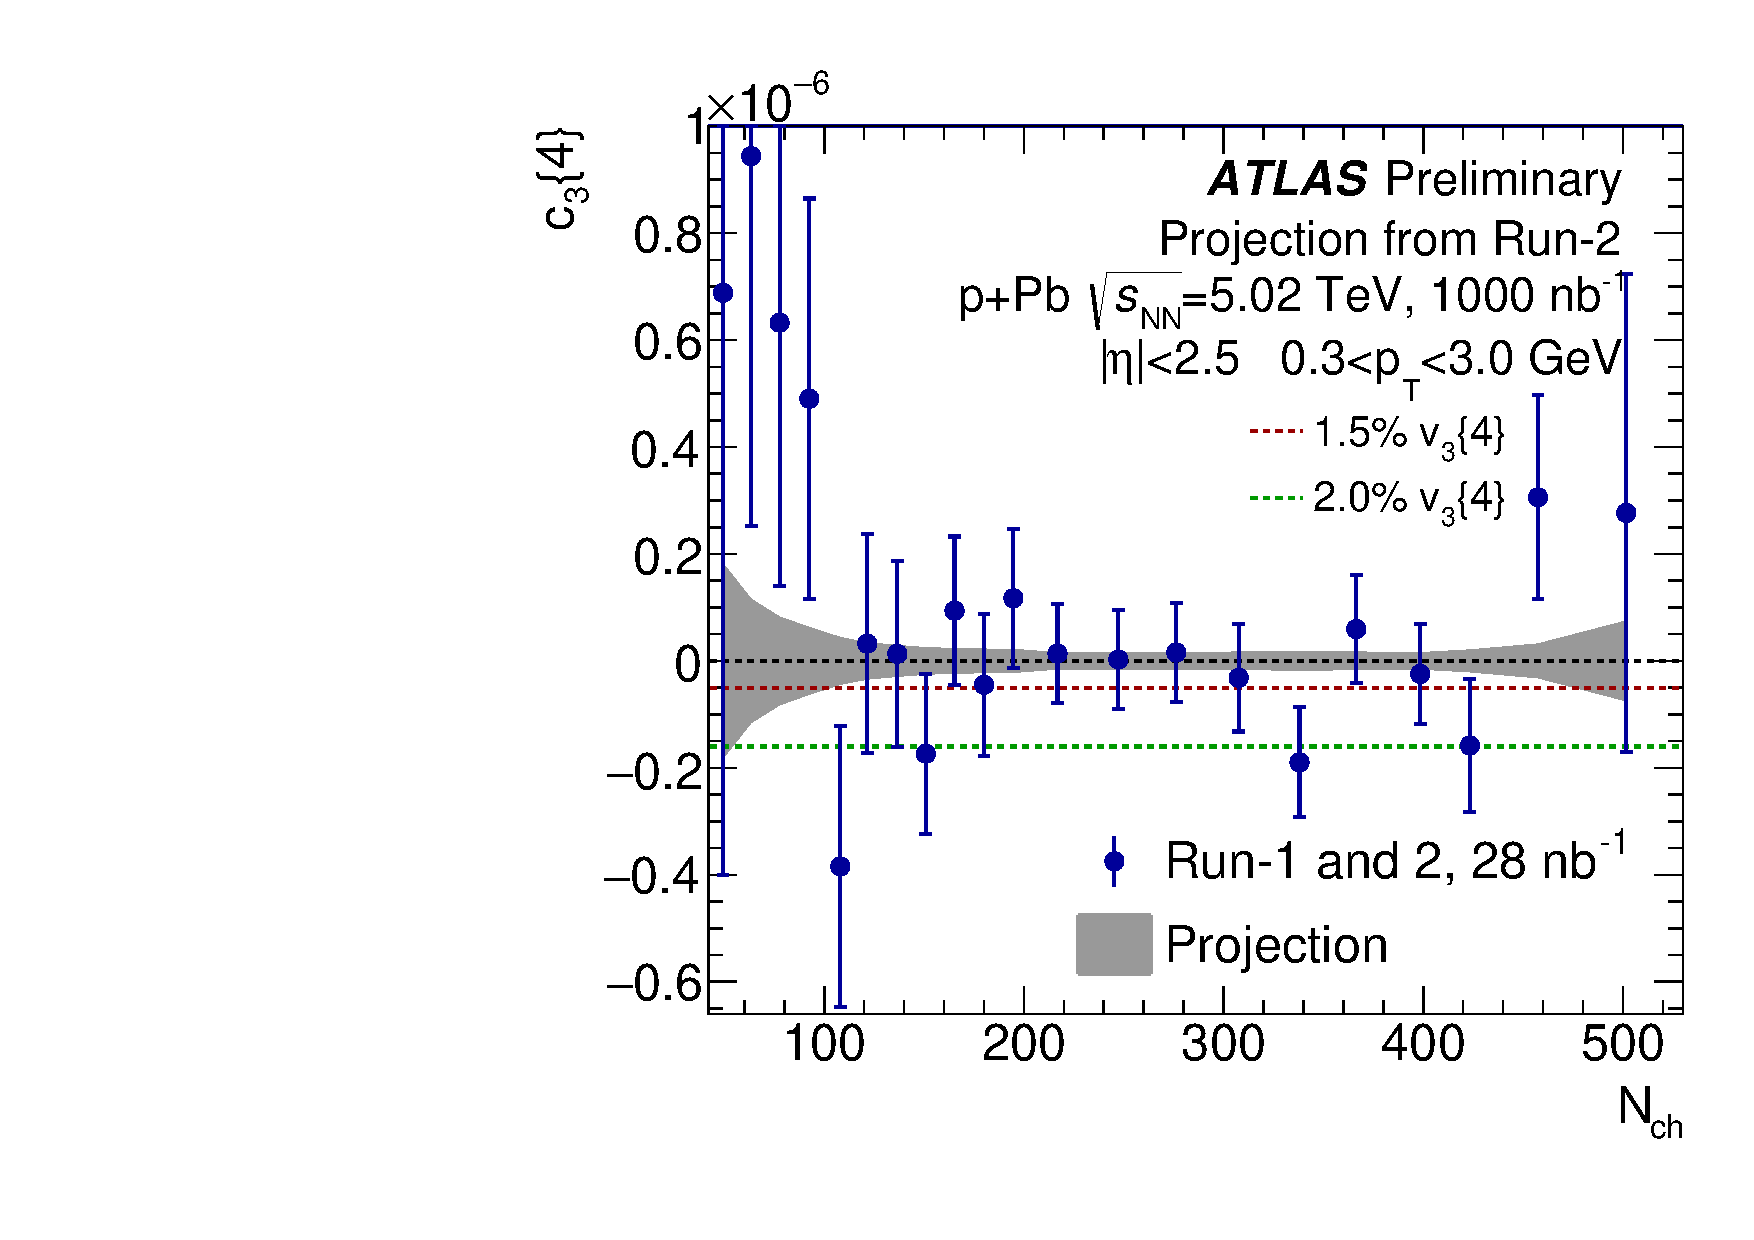
\includegraphics[width=.475\linewidth]{figs/chapter_subcumu/ATLAS_c34_pPb_proj.pdf}
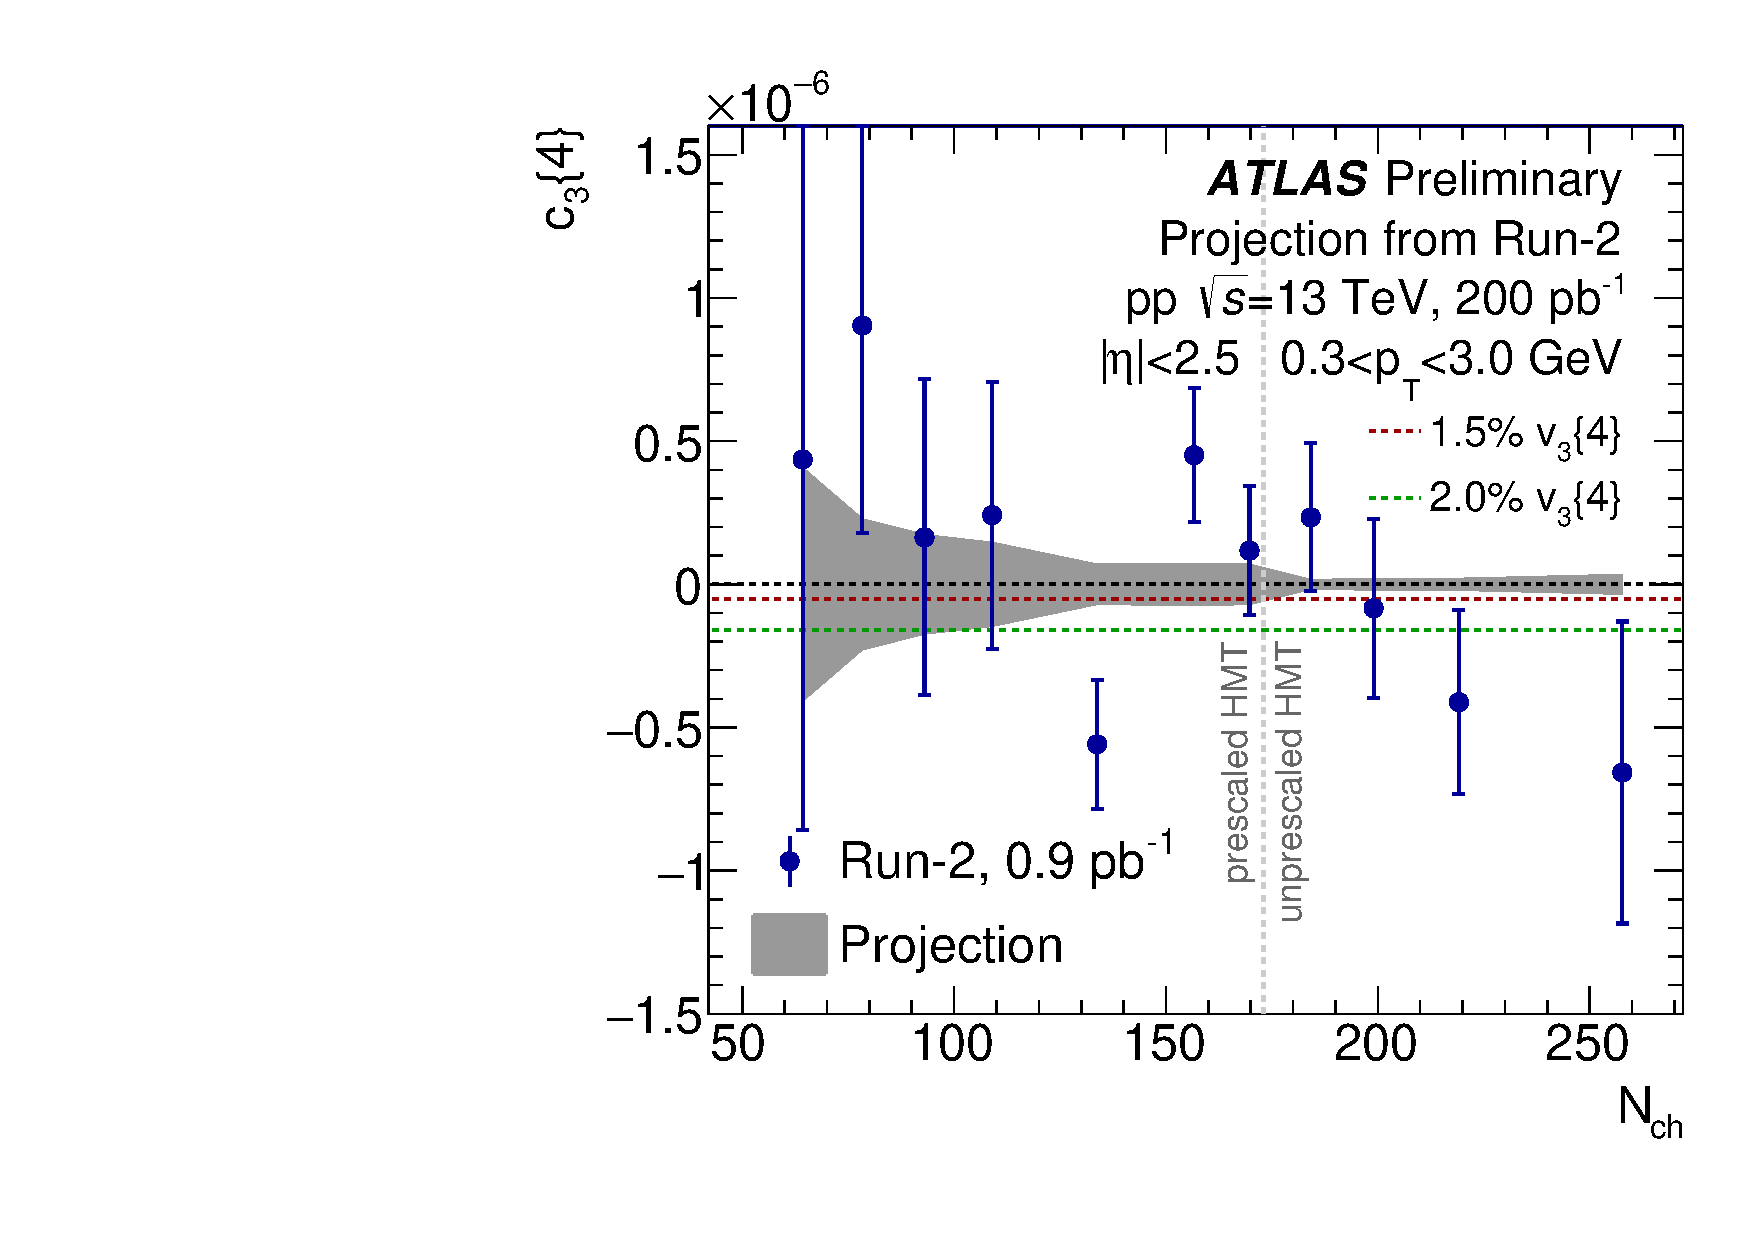
\includegraphics[width=.475\linewidth]{figs/chapter_subcumu/ATLAS_c34_pp_proj1.pdf}
\caption{4-particle cumulants $c_3\{4\}$ measured with three-subevent method for $p$+Pb (left) and $pp$ (right) collisions. Only statistical uncertainties are shown and the gray band represents the projected statistical uncertainty, with $c_3\{4\}$ assumed to be zero. The red and green dash lines represent $1.5\%$ and $2.0\%$ $v_3\{4\}$ signal, respectively. The vertical line indicates the transition between minimum-bias and HMT data.}
\label{fig:subcumu_ATLAS_c34_proj1}
\end{figure}

Figure~\ref{fig:subcumu_ATLAS_c34_proj2} illustrates the reduction of the statistical uncertainty due to the larger tracker acceptance in Run 4 for ATLAS. For this 4-particle correlator a reduction of the uncertainties of about 2.5 is expected, and therefore even the measurement of a $1\%$ $v_3\{4\}$ signal comes into reach. The influence of the acceptance increase on the uncertainties of 6- and 8-particle cumulants will be larger, factor of 4 and 6.5, respectively.

\begin{figure}[H]
\centering
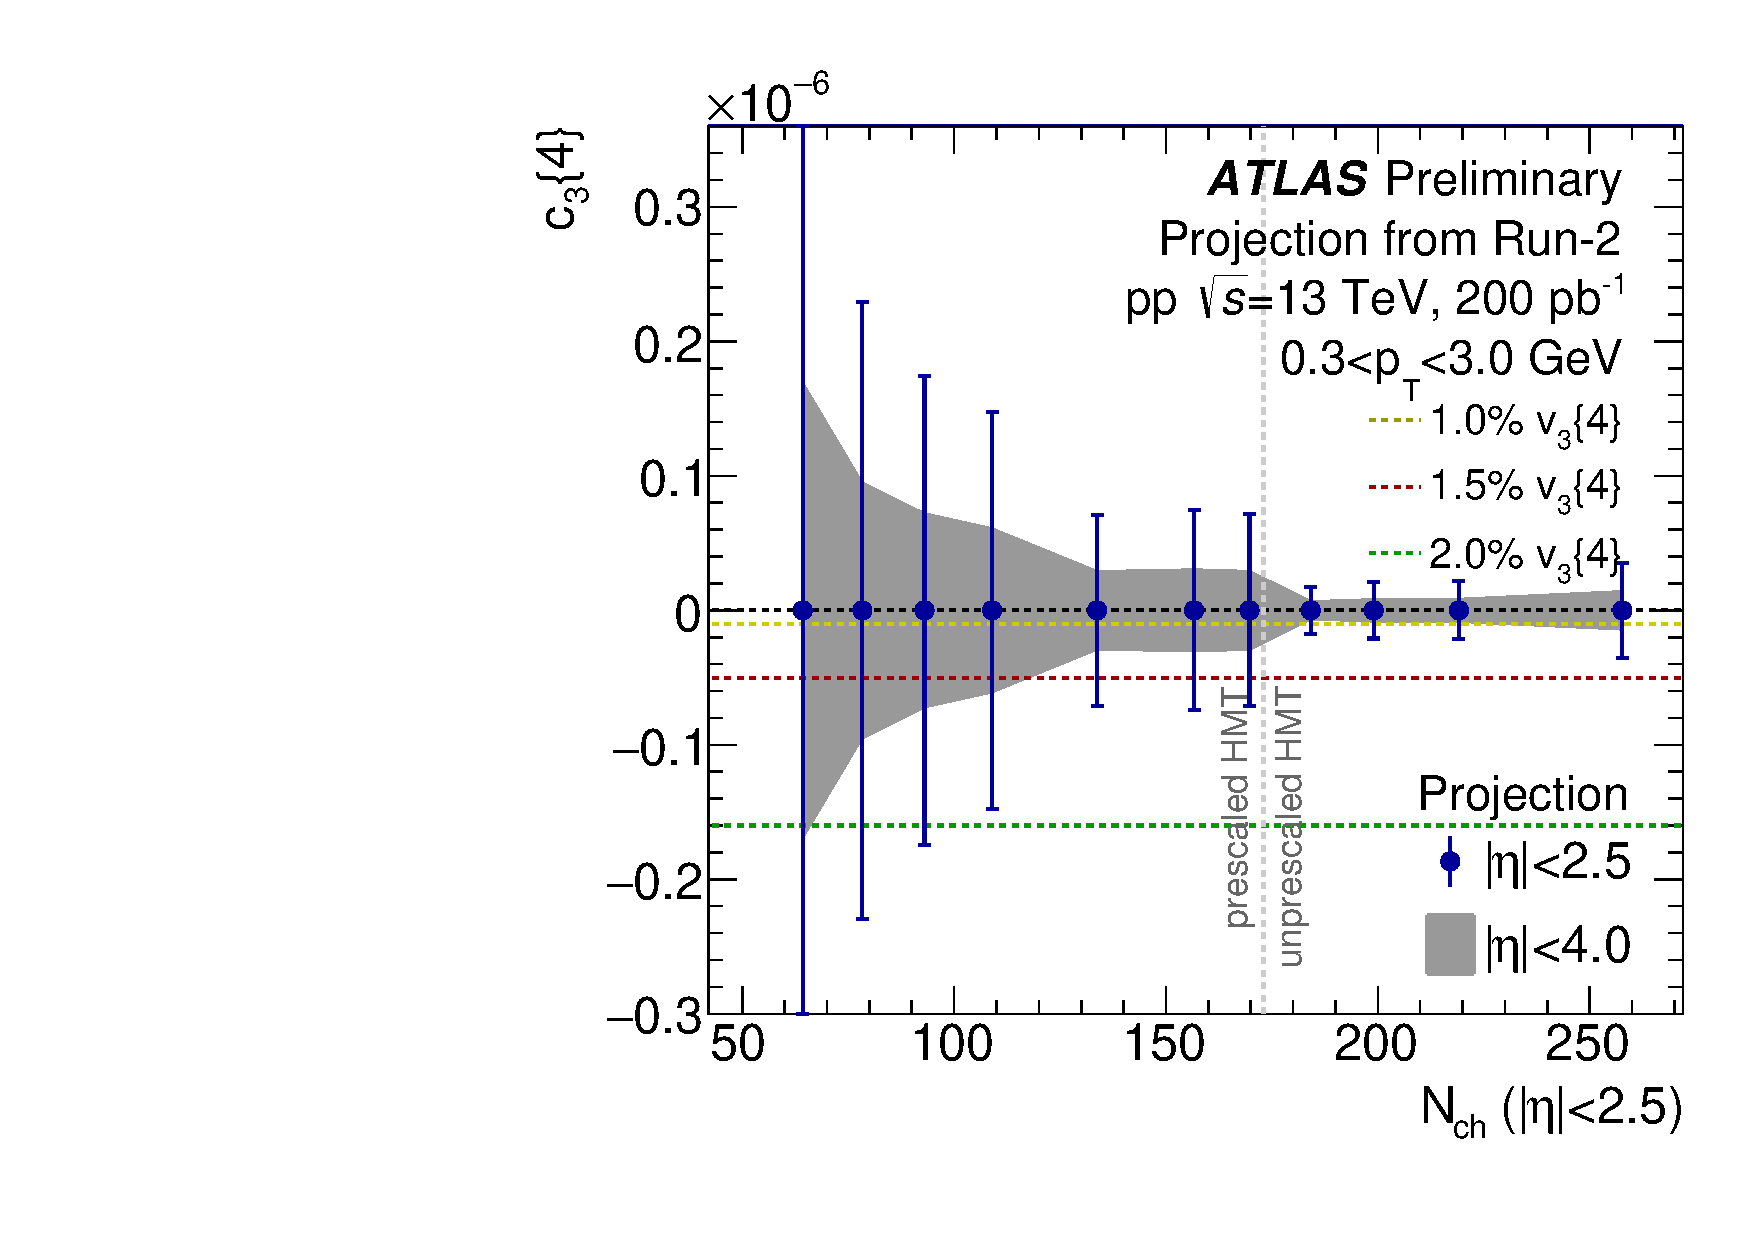
\includegraphics[width=.475\linewidth]{figs/chapter_subcumu/ATLAS_c34_pp_proj2.pdf}
\caption{Demonstration of the influence of the larger tracking acceptance for ATLAS in Run 4. 4-particle cumulant $c_3\{4\}$ for $pp$ collisions. The data points indicate the reach with the detector in Run 3 ($|\eta|<2.5$) while the grey band the enlarged acceptance of $|\eta|<4$ in Run 4. The yellow, red and green dash lines represent $1.0\%$, $1.5\%$ and $2.0\%$ $v_3\{4\}$ signal, respectively.}
\label{fig:subcumu_ATLAS_c34_proj2}
\end{figure}



\subsubsection{Correlation between flow harmonics}

Our studies show that nonflow contributions significantly affect the $c_n\{4\}$ measurements in small systems. In principle, all other similar cumulants measurements can also be affected. For instance, the four-particle symmetric cumulants $sc_{n,m}\{4\}=\lr{v_n^2 v_m^2}-\lr{v_n^2}\lr{v_m^2}$ quantify the lowest-order correlation between $v_n$ and $v_m$~\cite{Bilandzic:2013kga}. The three particle asymmetric cumulants such as $ac_n\{4\}=\lr{v_n^2 v_{2n} \cos 2n(\Phi_n-\Phi_{2n})}$ are sensitive to correlations involving both the flow magnitude $v_n$ and flow phase $\Phi_n$~\cite{Jia:2017hbm}. Extending subevent method to these observables is straightforward.

Figure~\ref{fig:subcumu_ATLAS_sc23_pp} compares the $sc_{2,3}\{4\}$ values obtained from the standard, two-, three-, four-subevent methods from $pp$ collisions in $0.3<\pT<3.0$ GeV (left panel) and $0.5<\pT<5.0$ GeV (right panel)~\cite{Aaboud:2018syf}. The values from the standard method are positive over the full $\Nch$ range, and are larger at lower $\Nch$ or in the higher $\pT$ range. This behavior suggests that the $sc_{2,3}\{4\}$ values from the standard method in $pp$ collisions, including those from Ref.~\cite{Sirunyan:2017uyl}, are strongly influenced by nonflow effects in all $\lr{\Nch}$ and $\pT$ ranges~\cite{Huo:2017nms}. In contrast the values from the subevent methods are negative over the full $\lr{\Nch}$ range, and they are slightly more negative at lowest $\lr{\Nch}$ and also more negative at higher $\pT$ region of $0.5<\pT<5.0$ GeV, results from the two-subevent method are systematically lower than those from the three- and four-subevent methods, suggesting that the two-subevent method may be affected by negative nonflow contributions. Such negative nonflow correlation has been observed in a PYTHIA calculation~\cite{Huo:2017nms}.

\begin{figure}[H]
\centering
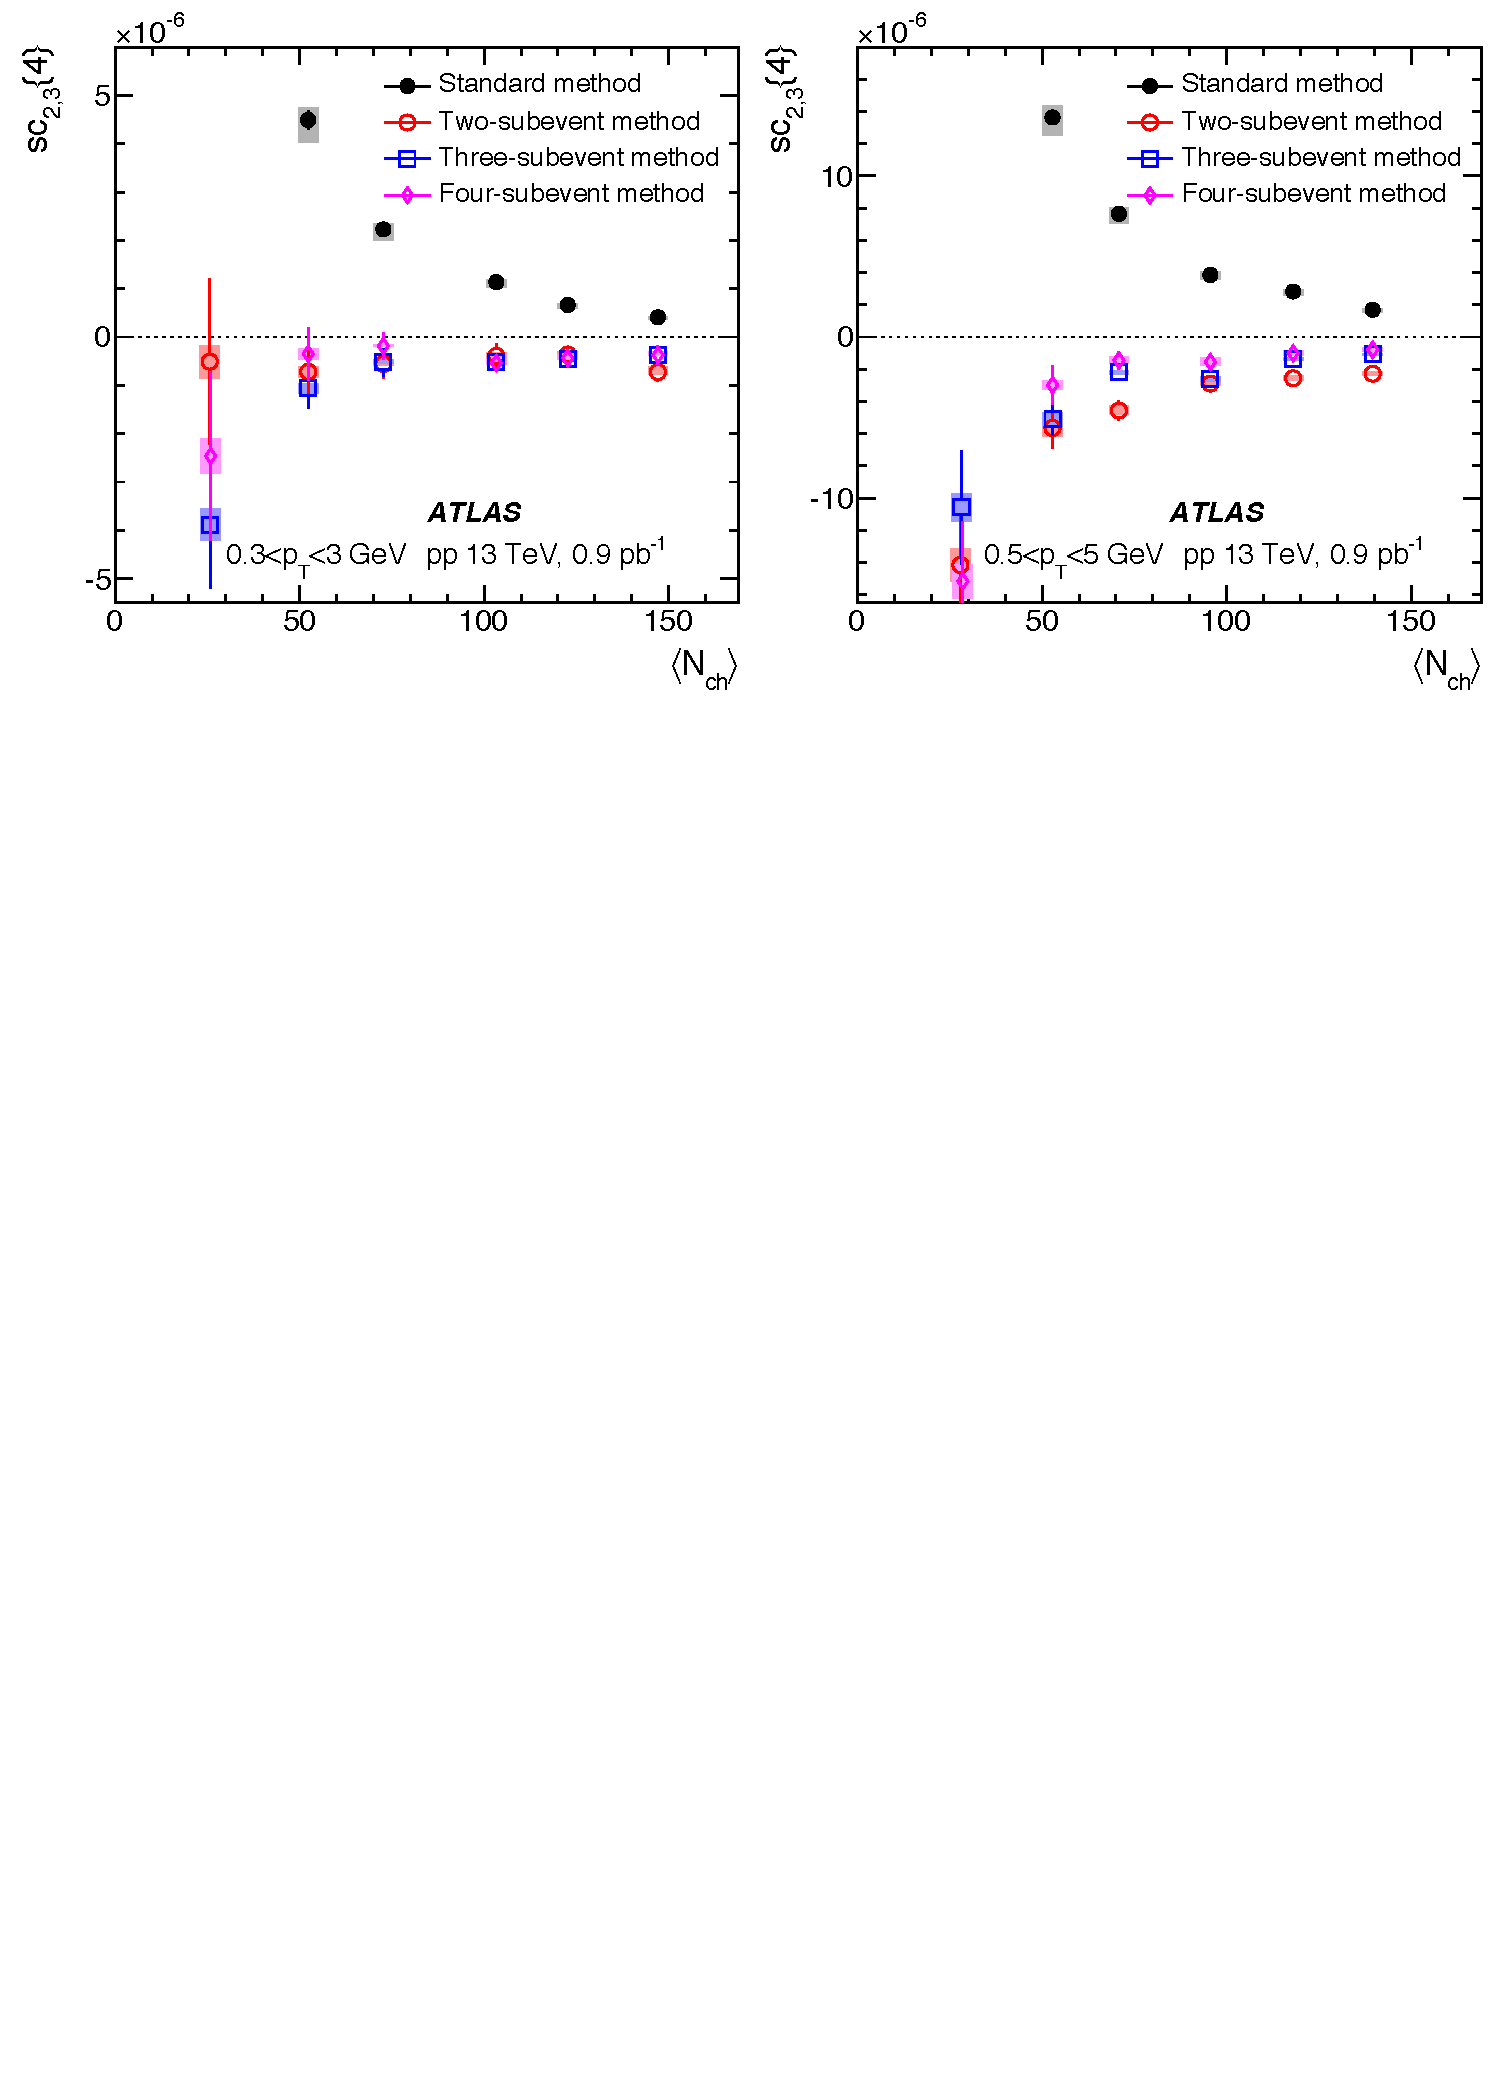
\includegraphics[width=.95\linewidth]{figs/chapter_subcumu/ATLAS_sc23_pp.pdf}
\caption{The symmetric cumulant $sc_{2,3}\{4\}$ as a function of $\Nch$ for $0.3<\pT<3.0$ GeV (left) and $0.5<\pT<5.0$ GeV (right) obtained for $pp$ collisions. The error bars and shaded boxes represent the statistical and systematic uncertainties, respectively. This figure is taken from Ref.~\cite{Aaboud:2018syf}.}
\label{fig:subcumu_ATLAS_sc23_pp}
\end{figure}

The results for the asymmetric cumulant $ac_2\{3\}$ are presented in Figure~\ref{fig:subcumu_ATLAS_ac24_pp}. The results are obtained from the standard, two-subevent, and three-subevent methods from $pp$ collisions in $0.3<\pT<3.0$ GeV (left) and $0.5<\pT<5.0$ GeV (right)~\cite{Aaboud:2018syf}. The results are positive for all methods. The results from the standard method are much larger than those from the subevent methods, consistent with the expectation that the standard method is more affected by nonflow correlations from dijets. Significant differences are also observed between the two-subevent and three-subevent methods at low $\lr{\Nch}$, but there differences decrease and disappear at $\lr{\Nch}>100$. The $ac_2\{3\}$ values from the three-subevent method show a slight increase for $\lr{\Nch}<40$ but are nearly constant for $\lr{\Nch}>40$. This behavior suggests that in the three-subevent method, the nonflow contribution may play some role at $\lr{\Nch}<40$, but is negligible for $\lr{\Nch}>40$. Therefore, the $ac_2\{3\}$ from the three-subevent method supports the existence of a three-particle long-range collective flow that is nearly independent of $\lr{\Nch}$ in $pp$ collisions, consistent with the $\lr{\Nch}$-independent behavior of $v_2$ and $v_4$ observed previously in the 2PC analysis~\cite{Aaboud:2016yar}.

\begin{figure}[H]
\centering
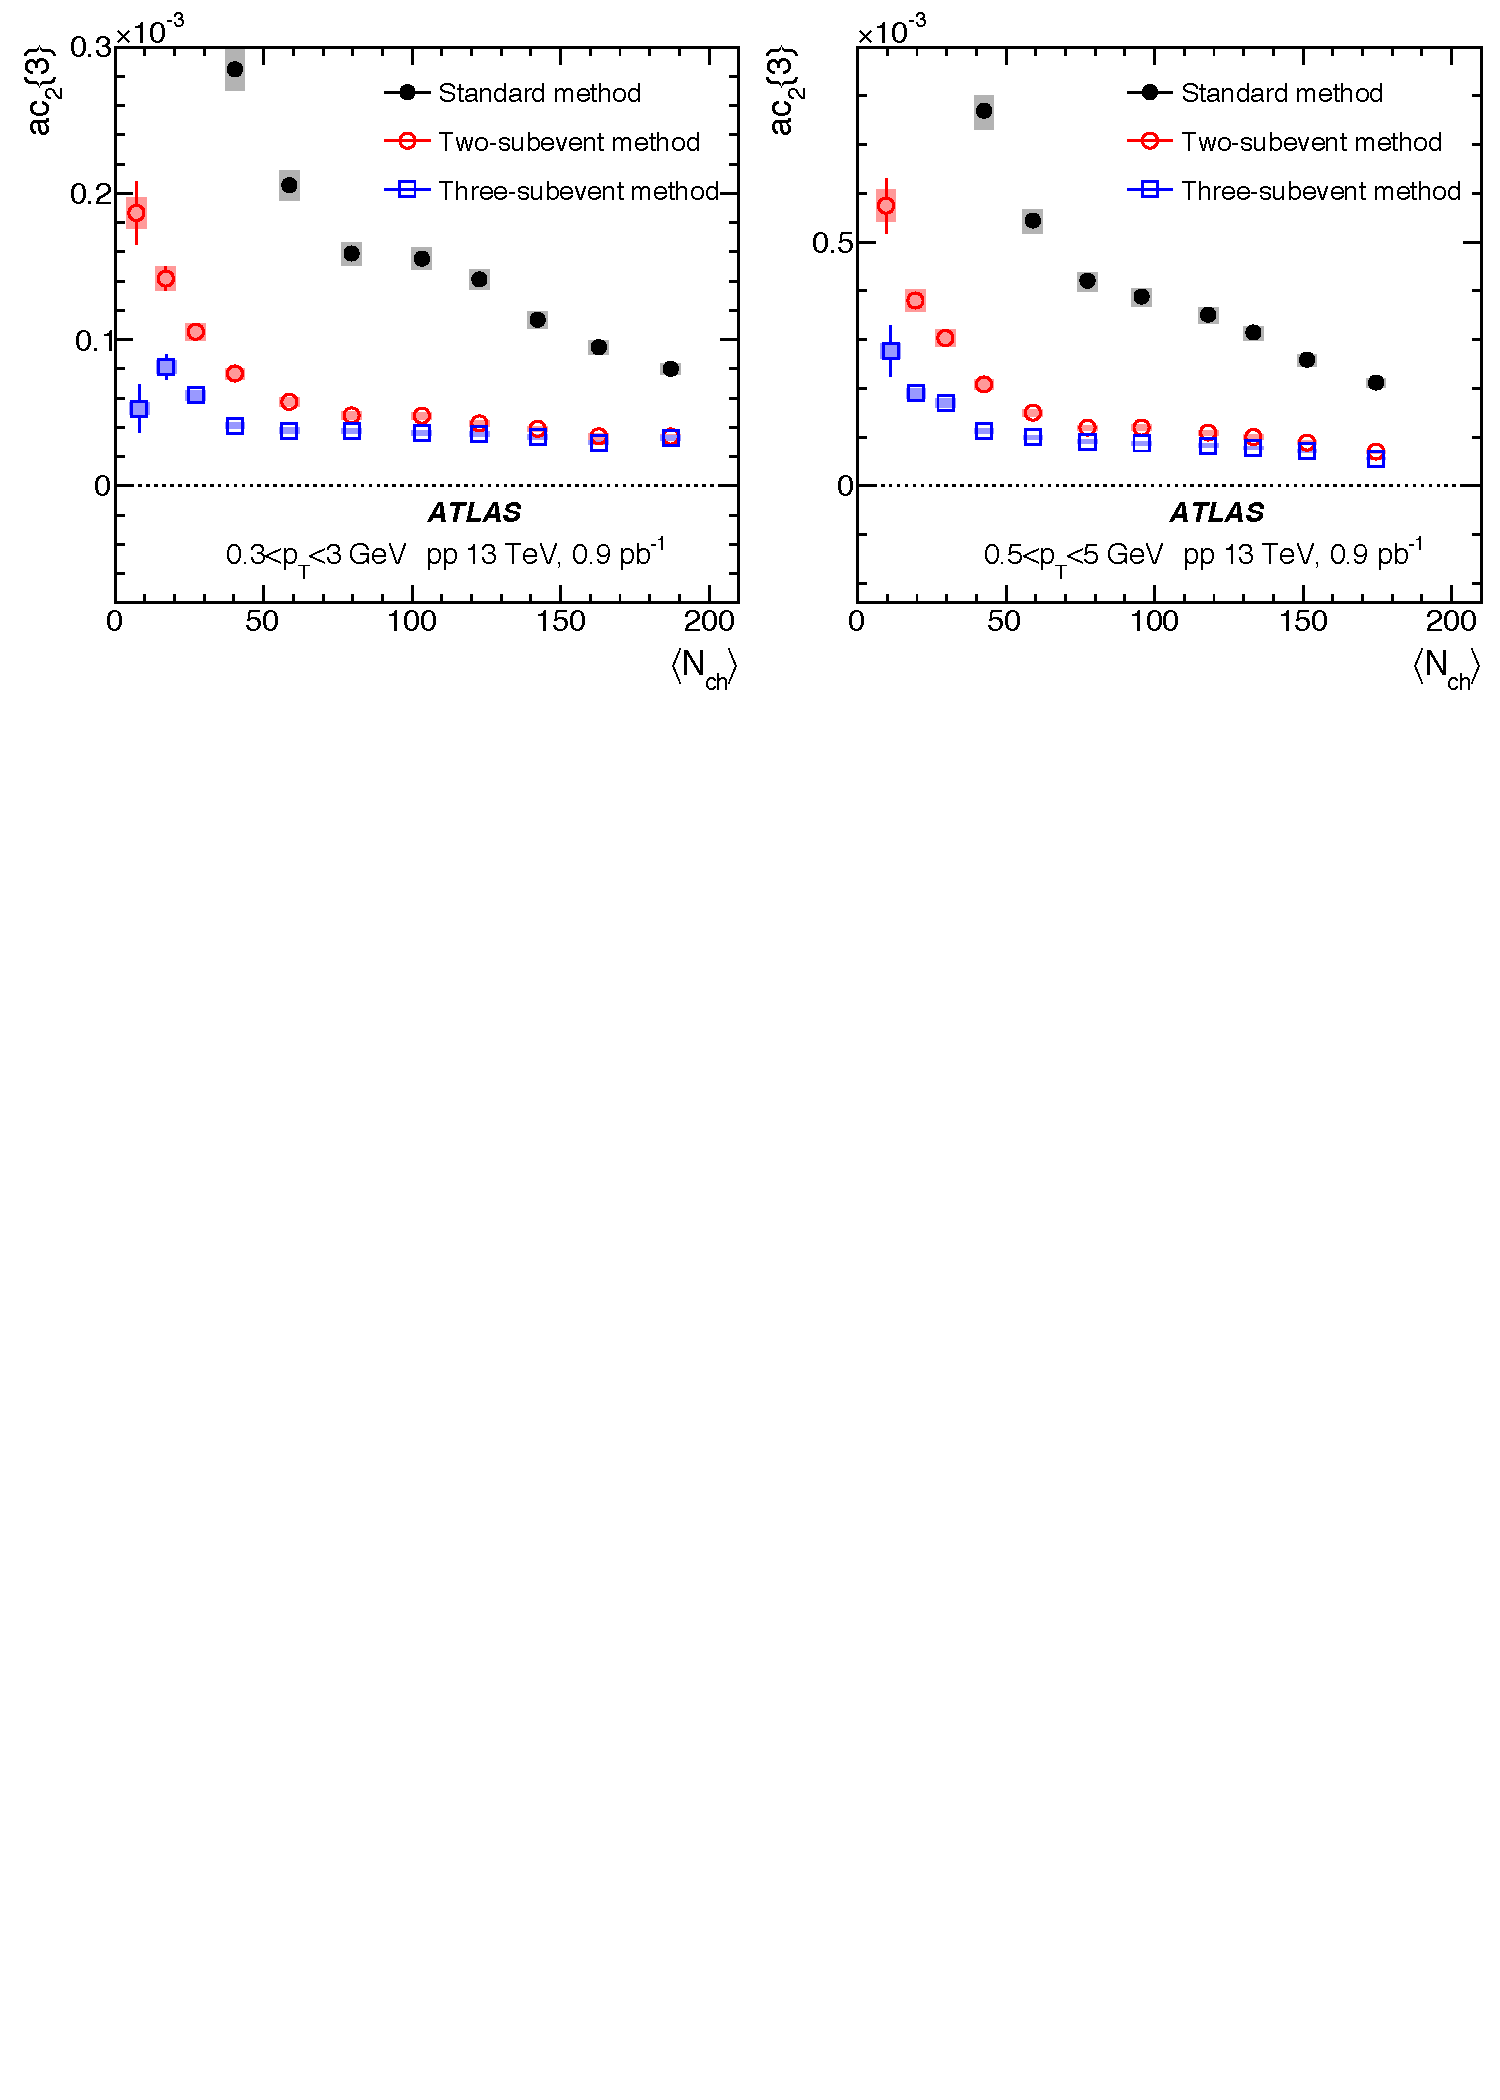
\includegraphics[width=.95\linewidth]{figs/chapter_subcumu/ATLAS_ac24_pp.pdf}
\caption{The symmetric cumulant $ac_2\{3\}$ as a function of $\Nch$ for $0.3<\pT<3.0$ GeV (left) and $0.5<\pT<5.0$ GeV (right) obtained for $pp$ collisions. The error bars and shaded boxes represent the statistical and systematic uncertainties, respectively. This figure is taken from Ref.~\cite{Aaboud:2018syf}.}
\label{fig:subcumu_ATLAS_ac24_pp}
\end{figure}



\subsubsection{Flow decorrelation}
\label{sec:flow_decorrelation}

In our studies, subevent is defined by $\eta$, which can potentially introduce longitudinal flow decorrelation effect~\cite{Aaboud:2017tql}. To be more specific, take asymmetric cumulant $ac_2\{3\}$ as one example. Three-subevent $ac_2\{3\}$ is defined as:
\begin{equation}
ac_2\{3\} = \lr{\lr{e^{\text{i}n(2\phi_2^a + 2\phi_2^b - 4\phi_4^c)}}}
\end{equation}
where $a$, $b$ and $c$ denote the three subevents. There are three possible distinct combinations of $\eta$ ranges:
\begin{itemize}
\item Subevent $c$ defined in forward pseudorapidity: $2.5/3 < \eta < 2.5$,
\item Subevent $c$ defined in backward pseudorapidity: $-2.5 < \eta < -2.5/3$,
\item Subevent $c$ defined in middle pseudorapidity: $-2.5/3 < \eta < 2.5/3$,
\end{itemize}
where the first two cases are symmetric, and they are combined and denoted as type 1. Third case is named as type 2. Measurement of flow decorrelation shows that both the flow amplitude and angle change as a function of $\eta$~\cite{Aaboud:2017tql}, thus different location of subevent $c$ could potentially lead to slightly different measurement of $ac_2\{3\}$.

To show the effects of flow decorrelation, Figure~\ref{fig:ATLAS_nac24_PbPb_decorr} shows the normalized $ac_2\{3\}$ from the standard method, compared with three-subevent method with $\phi_4$ defined in forward/backward $\eta$ and three-subevent method with $\phi_4$ defined in middle $\eta$. While values of three-subevent type 2 are consistent with standard cumulant, $ac_2\{3\}$ from three-subevent type 1 is slightly lower than the others. Since flow decorrelation is roughly linear as a function of $\eta$, type 1 will have the largest effects. For type 2, flow decorrelation effect in positive and negative $\eta$ are opposite sign and compensating with each other.

\begin{figure}[H]
\centering
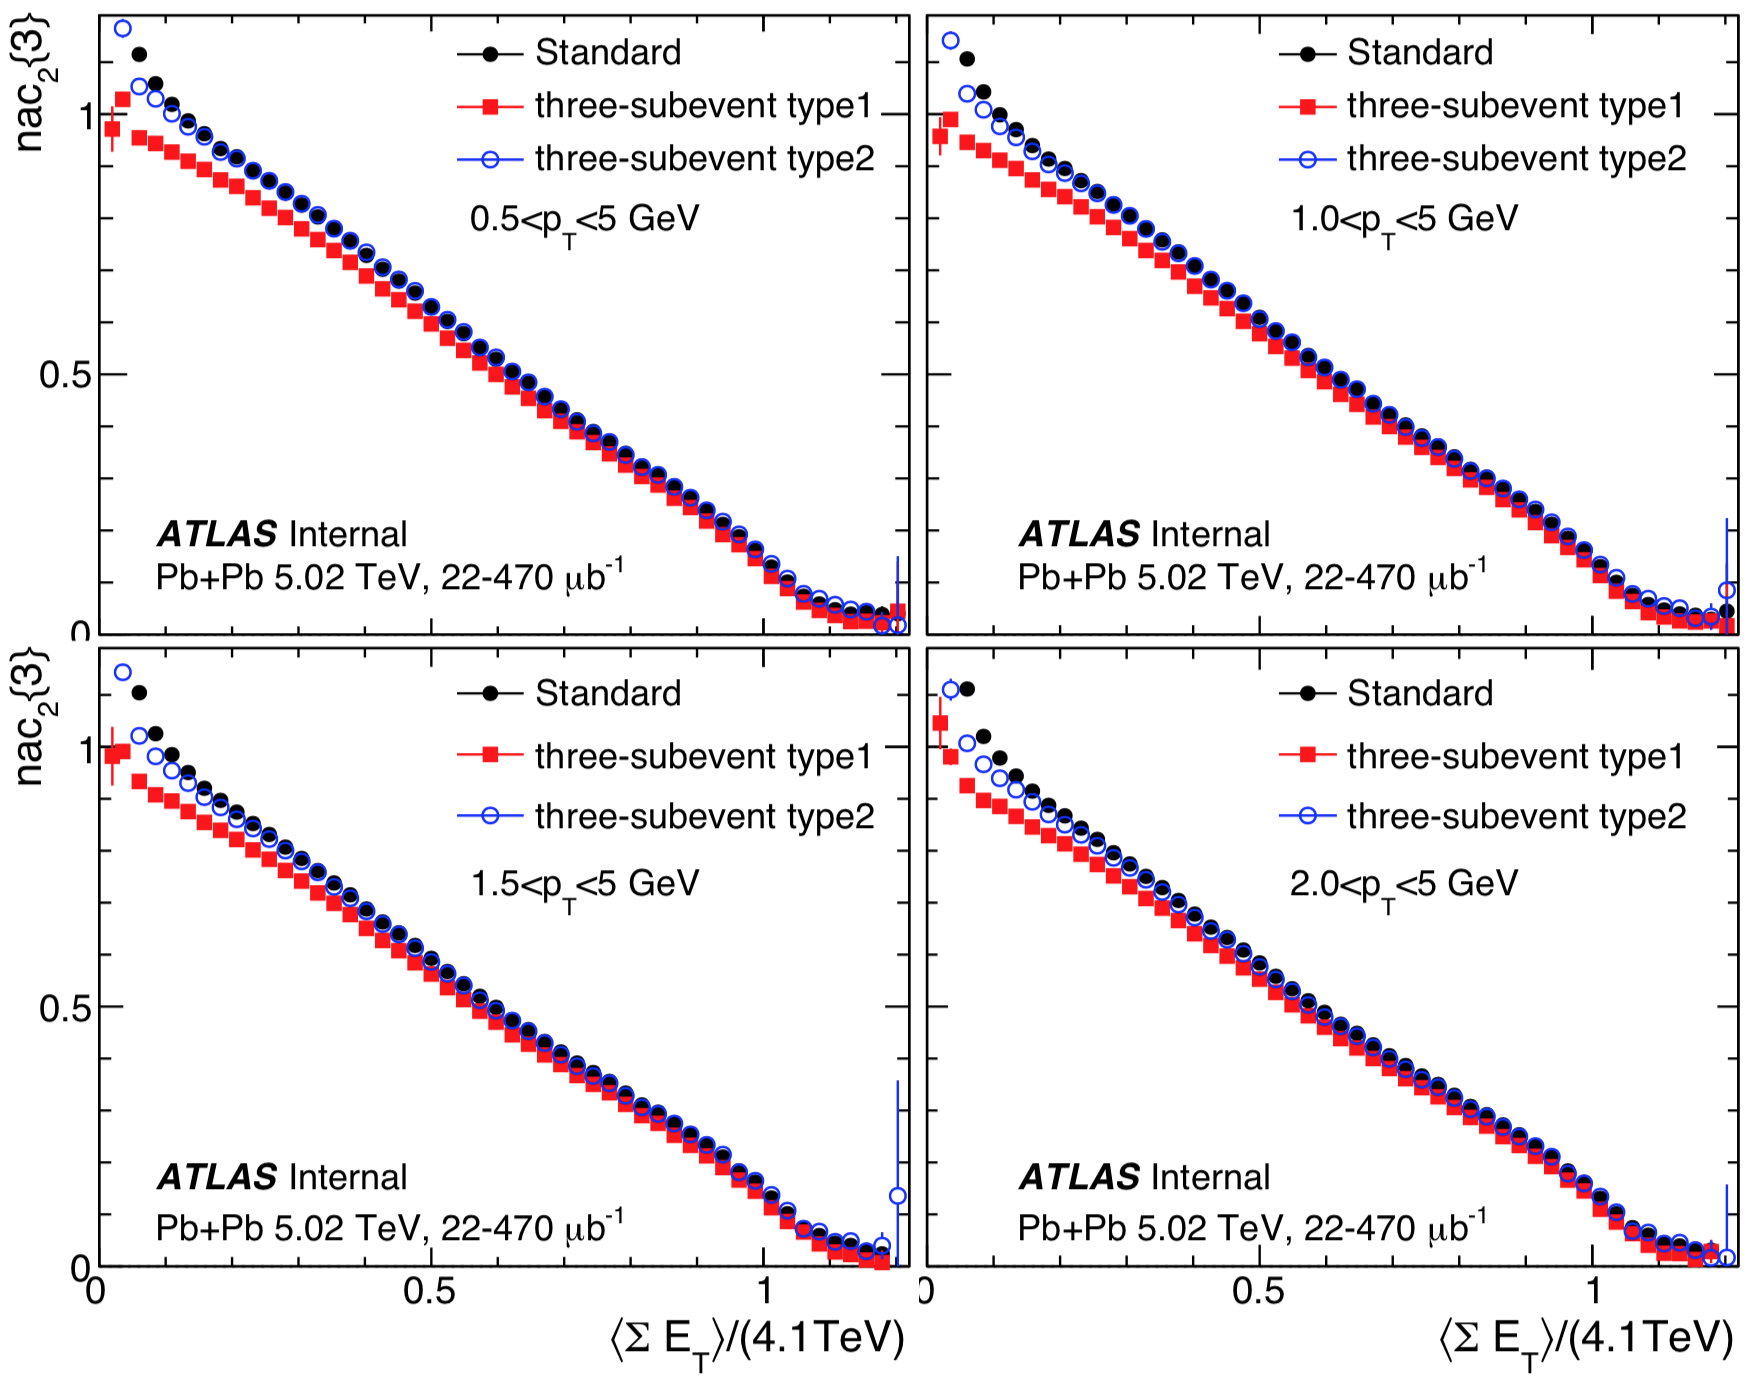
\includegraphics[width=.95\linewidth]{figs/chapter_subcumu/ATLAS_nac24_PbPb_decorr.png}
\caption{The normalized $ac_2\{3\}$ from the standard method (solid circles), three-subevent method with $\phi_4$ defined in forward/backward $\eta$ (solid squares) and three-subevent method with $\phi_4$ defined in middle $\eta$ (open circles). Different panels correspond to different $\pT$ ranges. Only statistical uncertainties are shown.}
\label{fig:ATLAS_nac24_PbPb_decorr}
\end{figure}

In our studies, by default type 1 and type 2 are combined to obtain the final results. In the future studies, the subevent method could provide an independent approach to measure the longitudinal flow fluctuation.










